%%%%%%%%%%%%%%%%%%%%%%%%%%%%%%%%%%%%%%%%%%%%%%%%%%%%%%%%%%%%%%%%%%% 
%                                                                 %
%                      THESIS MAIN FILE                           %
%                                                                 %
%%%%%%%%%%%%%%%%%%%%%%%%%%%%%%%%%%%%%%%%%%%%%%%%%%%%%%%%%%%%%%%%%%% 

% document definition
\documentclass[a4paper,11pt,chap,twoside]{thesis}

% also include the second line below.
\usepackage[hang]{caption2}
\usepackage{multirow}
\usepackage{subfigure}
\usepackage{float}

% to indent subsequent lines of captions
\renewcommand{\captionfont}{\bfseries}

% create the following file in the input from the template
\newcommand{\PaperTitle} {Accurate trajectory tracking on the KUKA youBot manipulator: Computed-torque control and Friction compensation}
\newcommand{\PaperSubject} {Accurate trajectory tracking on the KUKA youBot manipulator: Computed-torque control and Friction compensation}
\newcommand{\PaperTerm} {Summerterm 2018}		
\newcommand{\PaperDate} {\today}			
\newcommand{\ThesisAdvisor} {Prof. Dr. Paul G. Pl\"oger}
\newcommand{\ThesisReferee} {Prof. Dr. Roustiam Chakirov}
\newcommand{\ThesisExReferee} {M.Sc. Sven Schneider}
\newcommand{\PaperLecturerEMail} {mailto:paul.ploeger@smail.inf.h-brs.de}
\newcommand{\Paperkeywords} {Parameter estimation/identification, model-based controller, computed torque-control, friction modeling and compensation, rigid body dynamics and control}
\newcommand{\PaperMainWriter} {Jeyaprakash Rajagopal}
\newcommand{\PaperMainWriterEMail} {jeyaprakash.rajagopal@smail.inf.h-brs.de}
\newcommand{\ThesisAuthor} {Jeyaprakash Rajagopal}

%\usepackage[latin1]{inputenc} 

\usepackage[final]{graphicx}
%\usepackage{epstopdf}
\usepackage[hyphens]{url}

%\usepackage[expert,vargreek]{lucidbrb}

%\usepackage{mya4page} % not used, because now is implemented in the class 
\usepackage{amsmath}
%\usepackage{hyperref}
\usepackage{bibnames}
\usepackage{path}
\usepackage{subfigure}
\usepackage{fancyhdr}                    % Fancy Header and Footer 
\usepackage{tikz}
\usepackage{tikz-3dplot}
\usepackage[withpage]{acronym}
\usetikzlibrary{arrows,calc}
\usepackage{amsmath}
\usepackage[linesnumbered,ruled]{algorithm2e}
\usetikzlibrary{shapes,arrows}
%\usepackage{setspace}

%\usepackage{footmisc}
%\usepackage[perpage,symbol*]{footmisc} 


%---------------------------------------------------------------
\usepackage{color}
\definecolor{listinggray}{gray}{0.9}
%---------------------------------------------------------------
%\usepackage[copy=false, edit=false]{pdfcrypt}

%---------------------------------------------------------------
\usepackage{listings}
\lstset{language=Java}
\lstset{basicstyle=\footnotesize\small,%ttfamily,%\small,
tabsize=4,
tab=$\to$,
float=tbph,
extendedchars=true,
breaklines,
% prebreak={\space\MyHookSign},
% frame=single,
showtabs=false,
showspaces=false,
showstringspaces=false,
keywordstyle=\color{red}\bfseries,
identifierstyle=\bf\ttfamily,
aboveskip=\bigskipamount,
}
\lstset{captionpos=b}
\lstset{keywordstyle=\color{blue}\bfseries\bf}
\lstset{backgroundcolor=\color{listinggray}, rulecolor=\color{blue}}
\lstset{linewidth=\textwidth}
\lstset{stepnumber=5}
\lstset{numbers=left}
\lstset{numberstyle=\tiny\color{blue}}
\lstset{commentstyle=\color{magenta}\textit, stringstyle=\upshape,
	showstringspaces=false}
\lstset{frame=trBL,frameround=tttt}
%---------------------------------------------------------------

%% Hyperref setup
\usepackage{hyperref}
\hypersetup{
	 a4paper,
   colorlinks=true,
   linkcolor=black,
   filecolor=black,
   citecolor=black,
   urlcolor=black,
   plainpages=false,
   pdftitle={ \PaperTitle },
   pdfsubject={ \PaperSubject },
   pdfauthor={ \ThesisAuthor <jeyaprakash.rajagopal@smail.inf.h-brs.de>},
   pdfkeywords={ \Paperkeywords },
   bookmarksnumbered=true,
   pdfpagemode=UseOutlines,
   pdfpagelayout=SinglePage,  
   bookmarksopen=true
}
%\usepackage[copy=true, edit=false, annotate=true]{pdfcrypt}


\begin{document}
\tikzstyle{block} = [draw, fill=white, rectangle, 
    minimum height=3em, minimum width=6em]
\tikzstyle{sum} = [draw, fill=white, circle, node distance=1cm]
\tikzstyle{input} = [coordinate]
\tikzstyle{output} = [coordinate]
\tikzstyle{pinstyle} = [pin edge={to-,thick,black}]
\tdplotsetmaincoords{70}{20}

%%%%%%%%%%%%%%%%%%%%%%%%%%%%%%%%%%%%%%%%%%%%%%%%%%%%%%%%%%%%%%%%%%% 
%                                                                 %
%                            TITLE PAGE                           %
%               Master's Thesis or Master's Project               %
%                                                                 %
%%%%%%%%%%%%%%%%%%%%%%%%%%%%%%%%%%%%%%%%%%%%%%%%%%%%%%%%%%%%%%%%%%% 

% Supply information for use on title page:    
\thesistitle{\bf Accurate trajectory tracking on the KUKA youBot manipulator: Computed-torque control and Friction compensation}
%used for the header
\thetitle{Accurate trajectory tracking on the KUKA youBot manipulator: Computed-torque control and Friction compensation}         
\author{\ThesisAuthor}        
\degree{Master of Science in Autonomous System}
\thadviser{\ThesisAdvisor}
\cothadviser{\ThesisReferee}
\exthadviser{\ThesisExReferee}
\submitdate{Aug 15, 2018}
\copyrightyear{2018}   % if omitted, current year is used.        

% Print titlepage and other prefatory material:   
\titlepage        
%\copyrightpages
\emptypage         %optional 
\statementpage         
\emptypage
% toc, abstract, acknowledgement 
\singlespace 
%%%%%%%%%%%%%%%%%%%%%%%%%%%%%%%%%%%%%%%%%%%%%%%%%%%%%%%%%%%%%%%%%%% 
%                                                                 %
%                            ABSTRACT                             %
%                                                                 %
%%%%%%%%%%%%%%%%%%%%%%%%%%%%%%%%%%%%%%%%%%%%%%%%%%%%%%%%%%%%%%%%%%% 
\specialhead{\abstractname}

%%%background
Accurate trajectory tracking control is a desirable quality for the robotic manipulators. Since the manipulators are highly non-linear due to the presence of structured (i.e. model errors), and unstructured uncertainties (i.e. friction), it becomes very difficult to achieve high-precision tracking in the manipulator joints. Most common solution to this problem is the computed-torque control scheme where the inclusion of the dynamic model linearizes the non-linear system. Disadvantage of this method is that the controller's performance in high-speed operations relies heavily on the accuracy of the dynamic model parameters. Model parameters provided by the manufacturers are generally not accurate, and thus the identification of link parameters becomes necessary. Additionally, inclusion of friction compensation terms in the dynamic model improves the controller's performance, and helps us in achieving better dynamics control of the manipulator. This work considers the implementation of both identification of the dynamic model parameters and computed-torque controller. The identification procedure is the continuation of the previous research where the geometric relation semantics and the dynamics of the system needed correction. Real concern in any of the robotics based applications is safety of the hardwares used (i.e. motors, sensors) because they are generally quite expensive. So, this work gives highest priority regarding safety of the real system and the safety control layer monitors the state of the joints with the help of the encoder data such as joint positions, velocities and torques. The model-based controller uses the dynamic model of the youBot manipulator and feed-forward torques are computed by using the inverse dynamics solver based on a library. There are two kinds of control schemes considered in this work such as the basic and the alternate control. The alternate control method is chosen over the basic method, because the basic approach suffers in predicting the model torques due to the presence of inaccurate dynamic model parameters. Both of the schemes implement the same cascade PI controller which is the combination of both the position and velocity controllers for the purpose of better disturbance rejection. Controller gains are tuned empirically to the optimum for most controlwise challenging joints on the end of the kinematic chain. This work reports analysis on the semantics used by the existing rigid-body algorithms and these findings are useful in constructing the geometrical relation semantics between rigid bodies without introducing the logical errors. Then, a safety control check is performed in the real system that handles the breaches in the safety limit of the manipulator joints effectively with an understandable latency issues due to the use of non real-time operating system. The correctness of the dynamic model is tested with the gravity compensation task, and then the pure controller without the dynamic model is validated with the analytical trajectories. The friction modelling and compensation experiments are conducted in the basic control scheme implemented in this work. The computed-torque control scheme is evaluated on the farthest joints of the base with the help of the analytically formulated trajectories. In spite of using the inaccurate model parameters in the dynamic model, the controller tracks of the trajectory accurately with an acceptable tracking error on the manipulator joints.
\onehalfspace
\emptypage
%%%%%%%%%%%%%%%%%%%%%%%%%%%%%%%%%%%%%%%%%%%%%%%%%%%%%%%%%%%%%%%%%%% 
%                                                                 %
%                            ABSTRACT                             %
%                                                                 %
%%%%%%%%%%%%%%%%%%%%%%%%%%%%%%%%%%%%%%%%%%%%%%%%%%%%%%%%%%%%%%%%%%% 
\specialhead{NOTATIONS AND ACRONYMS}

\DeclareRobustCommand{\mL}{\mathcal{L}}

\textbf{\LARGE Notations}\\
\begin{table}[H]
\begin{tabular}{ll}
\boldmath{$q, \theta$} & \multicolumn{1}{l}{Joint Position} \\
\boldmath{$\dot{q}, \dot{\theta}, qd$} & \multicolumn{1}{l}{Joint velocity} \\ 
\boldmath{$\ddot{q}, \ddot{\theta}, qdd$} & \multicolumn{1}{l}{Joint acceleration} \\
\boldmath{$q_d, \dot{q}_d, \ddot{q}_d$} & \multicolumn{1}{l}{Desired joint position, velocity and acceleration} \\
\boldmath{$q_m, \dot{q}_m, \ddot{q}_m$} & \multicolumn{1}{l}{Measured joint position, velocity and acceleration} \\
\boldmath{$\tau$} & \multicolumn{1}{l}{Joint torque}\\
\boldmath{$\tau_m$} & \multicolumn{1}{l}{Model torque}\\
\boldmath{$\tau_f$} & \multicolumn{1}{l}{Friction torque}\\
\boldmath{$\tau_c$} & \multicolumn{1}{l}{Torque from the controller}\\
\boldmath{$rad$} & \multicolumn{1}{l}{Radians}\\
\boldmath{$rad/s$} & \multicolumn{1}{l}{Radians per second}\\
\boldmath{$[A]$} & \multicolumn{1}{l}{Orientation frame related to A}\\
\boldmath{$\{A\}$} & \multicolumn{1}{l}{Frame related to A}\\
\boldmath{$^AT_B$} & \multicolumn{1}{l}{Homogeneous transform from B to A}\\
\boldmath{$^AX_B$} & \multicolumn{1}{l}{General spatial transform from B to A}\\
\boldmath{$\psi$} & \multicolumn{1}{l}{Dynamic model parameters} \\
\end{tabular}
\end{table}

\begin{flushleft}
\textbf{\LARGE Acronyms} \\
\end{flushleft}

\begin{flushleft}
\begin{acronym}[JSONP]\itemsep0pt
\acro{DoF}{\textbf{D}egrees \textbf{o}f \textbf{F}reedom}
\acro{CoM}{\textbf{C}enter \textbf{o}f \textbf{M}ass}
\acro{Orocos}{\textbf{O}pen \textbf{Ro}bot \textbf{Co}ntrol \textbf{S}oftware}
\acro{KDL}{\textbf{K}inematics and \textbf{D}ynamics \textbf{L}ibrary}
\acro{PID}{\textbf{P}roportional \textbf{I}ntegral \textbf{D}erivative}
\acro{SP}{\textbf{S}et \textbf{P}oint}
\acro{PV}{\textbf{P}rocess \textbf{V}ariable}
\acro{CV}{\textbf{C}ontrol \textbf{V}ariable}
\acro{3-D}{3-\textbf{D}imensional}
\acro{w.r.t.}{\textbf{w}ith \textbf{r}espect \textbf{t}o}
\end{acronym}
\end{flushleft}

\emptypage
%%%%%%%%%%%%%%%%%%%%%%%%%%%%%%%%%%%%%%%%%%%%%%%%%%%%%%%%%%%%%%%%%%% 
%                                                                 %
%                         ACKNOWLEDGEMENT                         %
%                                                                 %
%%%%%%%%%%%%%%%%%%%%%%%%%%%%%%%%%%%%%%%%%%%%%%%%%%%%%%%%%%%%%%%%%%% 
 
\specialhead{ACKNOWLEDGMENTS}
 
I dedicate this thesis to my family and friends and I would like to thank all my supervisors for the guidance. My sincere thanks to Prof. Dr. Paul G. Pl\"oger for the support and guidance on both the RnD's and master thesis. I am thankful to Prof. Dr. Roustiam Chakirov for the valuable insights on my thesis. I am really grateful to M.Sc. Sven Schneider for keeping me in the right track throughout the course of these projects. I am grateful my fellow classmates of Master of Autonomous Systems for their support. My parents were also supporting during the course of MAS; I am grateful to them. 
\emptypage

\tableofcontents 
\pagestyle{plain}       
\newpage
\emptypage
%\listoftables          %required if there are tables
%\listoffigures         %required if there are figures


% the main contents %
%%%%%%%%%%%%%%%%%%%%%%%%%%%%%%%%%%%%%%%%%%%%%%%%%%%%%%%%%%%%%%%%%%%%%%%%%%%%%%%%%%%%%%%%%%%%%
% 																	INTRODUCTION																						%
%%%%%%%%%%%%%%%%%%%%%%%%%%%%%%%%%%%%%%%%%%%%%%%%%%%%%%%%%%%%%%%%%%%%%%%%%%%%%%%%%%%%%%%%%%%%%

%%%%%%%%%%%%%%%%%%%%%%%%%%%%%%%%%%%%%%%%%%%%%%%%%%%%%%%%%%%%%%%%%%%%%%%%%%%%%%%%%%%%%%%%%%%%%
% 															Chapter Introduction  																			%
%%%%%%%%%%%%%%%%%%%%%%%%%%%%%%%%%%%%%%%%%%%%%%%%%%%%%%%%%%%%%%%%%%%%%%%%%%%%%%%%%%%%%%%%%%%%%
\chapter{INTRODUCTION}

The industrial manipulators are highly non-linear dynamic systems in general, so it becomes difficult to achieve the high-performance trajectory tracking. Though many methods have been proposed by different authors, the computed-torque control is the the most common control scheme that is suitable for this kind of a problem. In spite of having many process control methods for the industrial robots, the PID controller is selected as the process control method and it is briefly explained in the next section. The computed-torque control method is advantageous than the pure PID control in many aspects such as the trajectory tracking control performance, lower feedback gains, lower energy consumption and the compliant motion~\cite{4586493}. This work aims to achieve the advanced model based controller scheme where the linear feedback control system is mandatory. There are two important aspects considered in the computed-torque control are the control law and dynamic model. Though this method is effective in accurate trajectory tracking, the manipulator is subject to uncertainties even in a well-defined industrial setup such as the accuracy of the model parameters and the unmodeled dynamics~\cite{trajectorytracking_nn}. The first uncertainty in the manipulator is that the model parameters provided by the manufacturers, these parameters are not accurate-enough and the findings on the same are presented by many researchers~\cite{muggler2013torque}~\cite{Atkeson}. The second uncertainty in the manipulator is unmodeled dynamics i.e. friction. The accurate model of the robot is mandatory as discussed in the previous section and the unavailability of the joint-torque sensors~\cite{torquecontrol} in the youBot manipulator joints makes the tracking control problem even harder. Apparently, there are only limited advantages of the computed-torque control strategy where the accuracy of the model parameters are not good enough. So, the accurate model parameters of the links are mandatory to solve this problem and it has been widely investigated by many researchers~\cite{Atkeson}~\cite{swevers} where the authors propose the identification procedure that can be used to estimate the model parameters of the system but there are many challenges involved in achieving it due to the presence of the implicit conventions, semantic problems and the trajectory selection criteria. The modified recursive Newton-Euler formulation is used for this purpose and then model fitting methods can be used to identify the model parameters of the links. This work attempts to deploy the estimated model parameters along with the friction compensation that brings us close in obtaining the complete dynamics of the system which in-turn provides the robust trajectory tracking in high-speed operations. The control can be considered in two different spaces such as

\begin{itemize}
\item \textbf{Joint space control }The joint controller contains the feedback control system that makes sure that the execution of the expected motion is being closely followed by the joint coordinates.
\item Whereas \textbf{in task/operational space control}, it is important to achieve the precise control of the end-effector motion for which the compliant motion control is necessary. The compliant control is nothing but having a proper algorithm that relates the interaction of the end-effector and the environment appropriately.
\end{itemize}

This work uses the joint space controller, so the torques can be commanded to the manipulator joints for executing the desired motion and it does not regulate the forces. The commanded torques go through an additional safety control layer that is implemented around the computed-torque control scheme. This layer performs the checking in all the three modes such as position, velocity and torque which depends particularly on the encoder data before applying the commanded torques to the manipulator joints. Feed-forward torques are generated through ID solver which is readily available in orocos KDL~\cite{smits2011kdl} library and the kinematic chain of the youBot manipulator needs to be created manually. There are two possible independent-joint control designs that can be used in a controller such as the independent single-joint and multi-joint model~\cite{Chung2016}. The independent single-joint model considers the dynamics of a single joint and it's response. Whereas the multi-joint model based control design considers the complete dynamic model of the robot. This work uses the multi-joint model where the interaction among the joints are handled. The desired end-effector motion can be executed by commanding the appropriate torques to the manipulator joints which depends on the motion plan in the joint level.

\section*{Mode of control}

The joint can be commanded with three kinds of inputs such as position, velocity and torque. So, a joint can be controlled in three different modes as depicted in Fig.~\ref{fig:modeofcontrol}.

\begin{figure}[h]
\centering
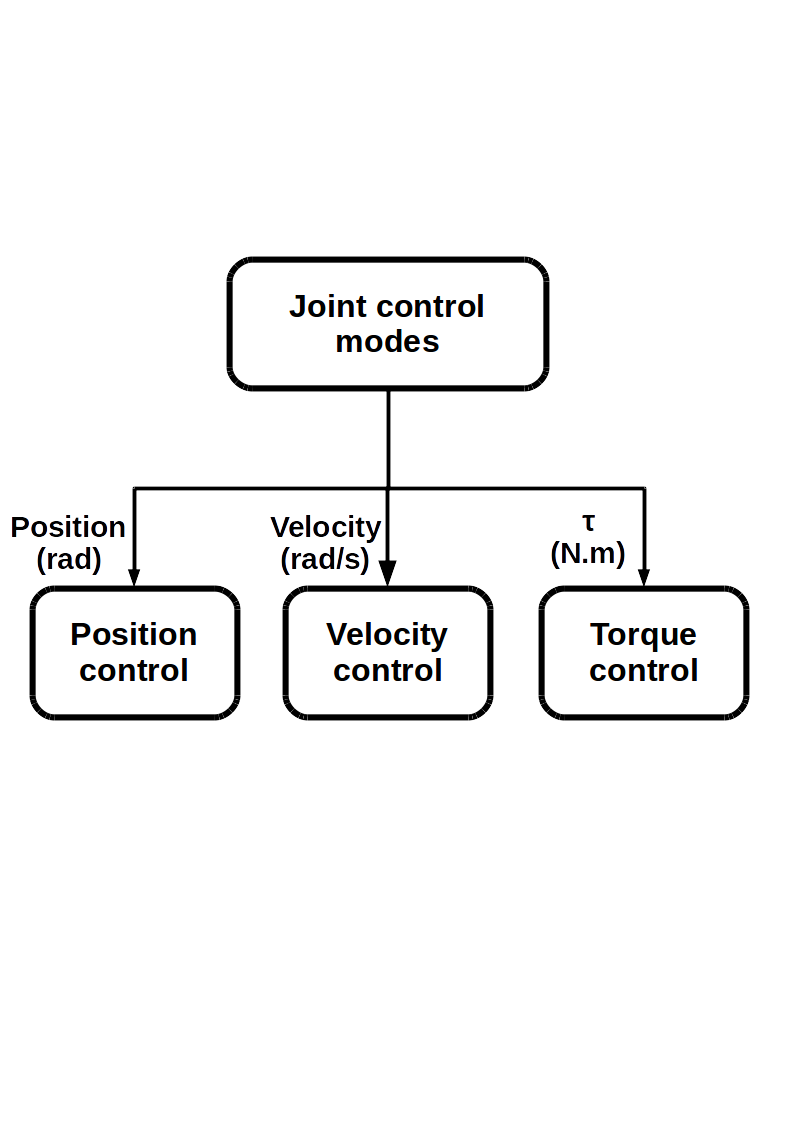
\includegraphics[width=80mm, trim=0 300 0 200]{pictures/joint_control_mode}
\caption{Joint's mode of control}
\label{fig:modeofcontrol}
\end{figure}

In position mode, a joint is commanded with position (joint angle in radians) to move the joint from a particular position to an another position. Whereas, the velocity mode commands the velocity to the joints for achieving the desired motion. The final classification is the torque control mode that commands the torque to the manipulator joints. The trajectory tracking errors can be efficiently minimized via torque mode since the dynamics and the joint configuration is considered~\cite{muggler2013torque}. Since, the motor takes the current as an input, the commanded joint torque has to be converted to target currents using a motor model based on the following equation~\eqref{eq:torquetocurrent}.

\begin{equation}
Current = (Commanded\_torque \times Gear\_ratio) / Torque\_constant (ampere)
\label{eq:torquetocurrent}
\end{equation}

The inverse of the above equation converts the current that is measured from the motors into joint torque. 

\begin{equation}
Torque= (Current \times Torque\_constant) / Gear\_ratio (Newton meters)
\label{eq:currenttotorque}
\end{equation}

The current to torque conversion as specified in the equation~\eqref{eq:currenttotorque} is particularly useful in interpreting the results of the system easily. The equations~\eqref{eq:torquetocurrent}~\eqref{eq:currenttotorque} are given based on the youbot driver\protect\footnotemark that is used in this work. \footnotetext[1]{\url{https://github.com/youbot/youbot_driver}} The torque control is quite robust and follows the trajectories in an accurate manner. This work uses the advanced model based torque controller and it is implemented in the joint space rather than the task space. This helps us in executing/tracking the trajectories in an accurately. This work assumes that the existing joint level controller gains are optimum hence the tuning the controller gains in the joint level is not the primary focus.

\section*{Control systems overview}
Basic definitions of this section are referred from~\cite{sellers2001overview}~\cite{astrom1995pid}. A system is considered to be linear when a change in output is directly proportional to the change in input. Since the robotic systems are highly non-linear, it is important to have the linear control strategy. This is achieved by using the linearization techniques that solves the non-linear systems problem. There are two kinds of control systems available such as open loop and the closed loop systems. Open loop, closed loop systems are depicted in the figures 1.2, 1.3 respectively. In the open loop systems, inputs are given to the system and the outcome is accepted regardless the deviations in the desired behaviour (feedback is not considered).

\begin{center}
\vspace{0.5cm}
\begin{tikzpicture}[auto, node distance=2cm,>=latex']
    \node [input, name=input] {};
    \node [block, right of=input, node distance=2.5cm] (robot){\textbf{Robot}};
	\node [output, right of=robot, node distance=2.9cm](output){};
	\draw [->,thick] (input) -- node {Desired} (robot);
    \draw [->,thick] (robot) -- node[pos=0.5] {Measured} (output);
\end{tikzpicture}
\captionof{figure}{Open loop system}
\vspace{0.5cm}
\begin{tikzpicture}[auto, node distance=2cm,>=latex']
    \node [input, name=input] {};
    \node [sum, right of=input, node distance=1.5cm] (minus) {\textbf{-}};
    \node [block, right of=minus, node distance=2.5cm] (control){\textbf{Controller}};
    \node [block, right of=control,
            node distance=3.5cm] (robot) {\textbf{Robot}};
	\node [output, right of=robot, node distance=2.9cm](output){};
	\draw [->,thick] (input) -- node {SP} (minus);
	\draw [->,thick] (minus) -- node {error} (control);
    \draw [->,thick] (control) -- node {CV} (robot);
    \draw [->,thick] (robot) -- node[pos=0.5] {PV} (output);
	\draw [->,thick] (output) -- ++ (0,-1.3) -| node [] {} (minus);
\end{tikzpicture}
\captionof{figure}{Closed loop system}
\end{center}

Whereas, the closed-loop control systems account the feedback of the system to minimize the deviations between the desired and observed data. This work uses the closed loop system for achieving the precise control of the manipulators.

\subsection*{PID controller}
The PID controller is the most commonly used controller in many of the industrial applications due to it's simplicity and it offers a lot of advantages such as fast response, brings the steady state error close to zero, avoiding oscillations and to achieve the stability in the system~\cite{temelp}~\cite{Chung2016}. It is possible to change the steady state response of the closed-loop system using this controller. The PID controller computes the error value between the desired and measured set-points repeatedly and it applies the correction based on the proportional(P), integral(I) and derivative(D) terms. P-term represents the current error that is being observed. I-term represents the history of errors which will be used to minimize the error between the expected set-point and it's response. D term is considered to predict the error based on it's rate of change in error. D term counteracts the overshoot caused by the P and I terms. The general mathematical representation of the complete PID control function can be expressed as follows

\begin{equation}
PV(t) = K_p\cdot error(t) + K_i\cdot \int_{0}^{t} e(t') dt' + K_d\cdot \frac{de(t)}{dt}
\end{equation}

It is possible to use different combinations within this controller depending on the requirements such as

\begin{itemize}
\item \textbf{P only control} is used in some specific applications where the feedback is expected to be constant.
\item \textbf{PI control} is commonly used controller.
\item \textbf{PD control} is used to control the servo motors.
\end{itemize}

The terms that are commonly used in the controller is depicted in the figure 1.3 and it is explained below

\begin{itemize}
\item Process Variable(\textbf{PV}) is the actual feedback that is being fed back to the controller from a process/system. 
\item Set Point(\textbf{SP}) is the desired variable for the process variable that is discussed above.
\item Control Variable(\textbf{CV}) is the actual output of the controller where the P, I and D terms are getting computed.
\item Error(\textbf{e}) is computed by finding the difference between SP and PV which can be a position or velocity set-point.
\item $K_p, K_i, K_d$ represents the proportional, integral and the derivative gains of the controller.
\begin{itemize}
\item If $K_p$ is high, the system oscillates a lot before reaching the desired setpoint which inturn introduces an offset in the system. 
\item $K_i$ tend to counteract this offset introduced by P control. If this gain value is high, the setpoint reaches the process variable faster.
\item $K_d$ tends to keep the stability of the system in control.
\end{itemize}
\end{itemize}

\subsubsection*{P control}

Proportional(P) control~\cite{temelp} is the linear feedback control system which produces an output that is proportion to the present error value(i.e. position set-point versus the control output). The proportion of the controller can be adjusted by multiplying the error with the proportional gain. By increasing the proportional gain, it is possible to reach the steady-state error faster but it must be considered with caution that the overshoot can occur with the higher P gains. This kind of control is applicable only when the system has a tolerance with the constant steady state error and the oscillations are not a big concern. The disadvantages of using the P controller are a lot of deviations where the stability of the system is compromised an the system overshoot.

\begin{center}
\begin{tikzpicture}[auto, node distance=2cm,>=latex']
    \node [input, name=input] {};
    \node [sum, right of=input, node distance=2cm] (minus) {\textbf{-}};
    \node [block, right of=minus, node distance=3cm, pin={[pinstyle]above:$K_p$}] (control){\textbf{P = ($K_p \times q_e$)}};
    \node [block, right of=control,
            node distance=3.5cm] (robot) {\textbf{Robot}};
	\node [output, right of=robot, node distance=2.9cm](output){};
	\draw [->,thick] (input) -- node {$q_d$} (minus);
	\draw [->,thick] (minus) -- node {$q_e$} (control);
    \draw [->,thick] (control) -- node {} (robot);
    \draw [->,thick] (robot) -- node[pos=0.5] {$q_m$} (output);
	\draw [->,thick] (output) -- ++ (0,-1.3) -| node [] {} (minus);
\end{tikzpicture}
\captionof{figure}{P Only controller}
\end{center}

\subsubsection*{PI control}
PI control depicted in Fig. 1.5 eliminates the steady state error from the P controller. The history are errors are accounted by the I controller to close the gap between the step input and it's response in the system. The P and I control terms together makes the system follow the step response quite closely. This reduces the overshooting and it helps achieving the stable system. This kind of a controller has no ability to predict the future errors(the rate of change in the error).

\begin{center}
\begin{tikzpicture}[auto, node distance=2cm,>=latex']
    \node [input, name=input] {};
    \node [sum, right of=input, node distance=2cm] (minus) {\textbf{-}};
    \node [block, right of=minus, node distance=2.5cm] (pcontrol){\textbf{P}};
    \node [block, above right of=minus, node distance=3.5cm] (icontrol){\textbf{I}};
    \node [sum, right of=minus, node distance=5.5cm](summation) {\textbf{$\epsilon$}};
    \node [block, right of=summation,
            node distance=3cm] (robot) {\textbf{Robot}};
	\node [output, right of=robot, node distance=2.9cm](output){};
	\draw [->,thick] (input) -- node {$q_d$} (minus);
	\draw [->,thick] (minus) -- node {$q_e$} (pcontrol);
	\draw [->,thick] (minus) |- node[pos=0.1] {} (icontrol);
	\draw [->,thick] (icontrol) -| node {} (summation);	
	\draw [->,thick] (pcontrol) |- node {} (summation);	
    \draw [->,thick] (summation) -- node {} (robot);
    \draw [->,thick] (robot) -- node[pos=0.5] {$q_m$} (output);
	\draw [->,thick] (output) -- ++ (0,-1.3) -| node [] {} (minus);
\end{tikzpicture}
\captionof{figure}{PI controller.}
\end{center}

\subsubsection*{PD control}

P-D controller depicted in Fig. 1.6 is used to increase the stability of the system with the inclusion of the derivative control or the damping factor to the proportional control.

\begin{center}
\begin{tikzpicture}[auto, node distance=2cm,>=latex']
    \node [input, name=input] {};
    \node [sum, right of=input, node distance=1.5cm] (minus) {\textbf{-}};
    \node [block, above right of=minus, node distance=2.9cm] (kp) {$K_p \cdot q_e$};
    \node [block, right of=minus, node distance=2.1cm] (kv) {$K_v \cdot \dot{q}_e$};
    \node [sum, right of=minus, node distance=4.5cm](summation) {$\epsilon$};
    \node [block, right of=summation,
            node distance=3.5cm] (robot) {\textbf{Robot}};
	\node [output, right of=robot, node distance=2.9cm](output){};
	\draw [->,thick] (input) -- node {$q_d, \dot{q}_d$} (minus);
	\draw [->,thick] (minus) |- node[pos=0.815] {$q_e$} (kp);
	\draw [->,thick] (minus) -- node {$\dot{q}_e$} (kv);
	\draw [->,thick] (kp) -| node {} (summation);
	\draw [->,thick] (kv) -- node {} (summation);	
	\draw [->,thick] (summation) -- node {} (robot);
    \draw [->,thick] (robot) -- node[pos=0.5] {$q_m, \dot{q}_m$} (output);
	\draw [->,thick] (output) -- ++ (0,-1.3) -| node [] {} (minus);
	\draw[dashed] (1.1,-1) -- (6.5,-1) -- (6.5,3.5) -- (1.1,3.5) -- (1.1,-1) node[pos=0.1] {\textbf{PD Control}};
\end{tikzpicture}
\captionof{figure}{PD control}
\end{center}

\section*{Friction modeling and compensation}

An important aspect that needs to be accounted in the dynamic model of the manipulator is friction~\cite{olsson1998friction}. Friction is a highly non-linear phenomenon that resists the relative motion of the rigid bodies and it can be classified into two categories such as static, kinetic friction. At first, the static friction is present when a rigid body attempts or putting an effort to move. Whereas dynamic or kinetic friction occurs when the rigid body is in motion and these two techniques are explained in detail in the preceding sections of this report. The frictional effect influences the manipulator performance in both the static and the dynamic configurations which could cause instability in the control. The friction can be compensated in two different ways such as model and non-model based scheme. The static friction estimates obtained manually through the automated testing in the previous work~\cite{RnD2Rajagopal} for the youBot manipulator and it is particularly useful in adding the compensation terms with the dynamic model of the manipulator.

\section*{Report structure}

The report outline is given as follows

\begin{itemize}
\item Section \hyperref[sec:stateoftheart]{2} state of the art on identification methods.
\item Section \hyperref[sec:approach]{3} describes the hardware, software platform and the approaches used in this work. It discusses semantics of the rigid-body algorithms, the computed-torque control along with the friction modeling and compensation terms, finally trajectory generation method for evaluating the controller.
\item Section \hyperref[sec:experiments]{4} discusses and presents the experimental results of this work.
\item Section \hyperref[sec:conclusion]{5} presents the conclusions and future work.
\end{itemize}
\emptypage
%%%%%%%%%%%%%%%%%%%%%%%%%%%%%%%%%%%%%%%%%%%%%%%%%%%%%%%%%%%%%%%%%%%%%%%%%%%%%%%%%%%%%%%%%%%%%
% 																STATE OF THE ART 																					%
%%%%%%%%%%%%%%%%%%%%%%%%%%%%%%%%%%%%%%%%%%%%%%%%%%%%%%%%%%%%%%%%%%%%%%%%%%%%%%%%%%%%%%%%%%%%%
\chapter{STATE OF THE ART}
\label{sec:stateoftheart}

The dynamic equations of kinematic chains of rigid bodies~\cite{swevers} represents the relationship between the motion of the system and the forces that cause it~\cite{craig2005introduction}. It can be considered as a mathematical model that computes forces and acceleration of the system which are relevant to the dynamics of the system. The computation of accelerations and forces based on two different algorithms can be named as forward and inverse dynamics respectively. Forward dynamics computes the accelerations based on the given joint position, velocity, torque inputs to produce the desired acceleration response in the system. It is mostly used in the simulation based systems. Whereas, inverse dynamics compute forces based on the given joint position, velocity and acceleration. These two algorithms have the system model that represents the physical properties of a system and the accuracy of the computations depend heavily on the model parameters. The algorithm that combines both the forward and inverse dynamics is referred as hybrid dynamics~\cite{featherstone2014rigid} where both the acceleration and force inputs are given to achieve a particular task. The equations of motion can be obtained through two different formulations such as the Newton-Euler and Lagrangian. Recursive Newton-Euler formulation is the most commonly used method~\cite{smits2011kdl}~\cite{featherstone2014rigid} since it is computationally efficient. The inverse dynamics computes the motion information of the rigid-body systems through the forward recursion that computes velocities and accelerations from proximal to distal links and a backward recursion is followed to compute the forces, torques from distal to proximal links. In~\cite{featherstone2014rigid}, author uses spatial vector form that combines the linear and angular aspects of motions, forces into a single six-dimensional vector and the computational efficiency increases with it. Complete dynamics of the system can be achieved by considering the uncertainties such as model errors, unmodeled dynamics~\cite{trajectorytracking_nn} which are present in the system. Model errors can be classified into kinematic and dynamic model errors but this work considers only dynamic model parameters. In~\cite{Atkeson}, author modifies the recursive Newton-Euler formulation to a linearized matrix-form for identifying the model parameters and the same method is used in the previous work~\cite{RnD2Rajagopal} where geometrical relation semantics of the rigid body are inaccurate and acceleration of the distal link that is being transmitted across joints due to the movement of the current joint is not accounted properly. In most of the rigid-body algorithms, inertial frame is attached to CoM of the rigid-body, but it is shifted to the joint origin by using the parallel-axis theorem. Re-expressing the inertia w.r.t. joint origin is essential due the unknown location of the CoM. The implementation is based on the coordinate calculations and the semantics checking is not the part of it. The numerical calculations consider the integration as an addition of two matrices but the semantics check ensures the physical meaning of those operations. The operations involved with the pose, motion and force transforms need to be semantically correct where the constraints are also applicable but the only use of numerical computations can introduce the logical errors in the system~\cite{geometicsemanticspart1}~\cite{geometicsemanticspart2}. The unknown dynamic model parameters are mass, CoM and moments of inertia and these parameters can be identified with the use of ridge regression. The kinematic chain that is created in the dynamic model based on Orocos KDL~\cite{smits2011kdl} needs correction in the frame assignments since the frame diagram in KDL is not matching with it's implementation. The friction phenomenon is one of the important effects that is present in the unmodeled dynamics. Static friction modeling has been done in the previous work~\cite{RnD2Rajagopal}. Friction modelling i.e. static friction models and the compensation~\cite{friction} techniques are discussed~\cite{corberan2012haptic}. Evolution of static friction model started with the static friction and Coulomb friction~\cite{olsson1998friction} which is the most simplified version of friction~\cite{swevers}. Then viscous friction is added with the static and Coulomb. Finally, static friction model includes the Stribeck effect along with the static and viscous friction. The model of friction that includes Stribeck friction is shown in the following figure

\begin{figure}[h]
\centering
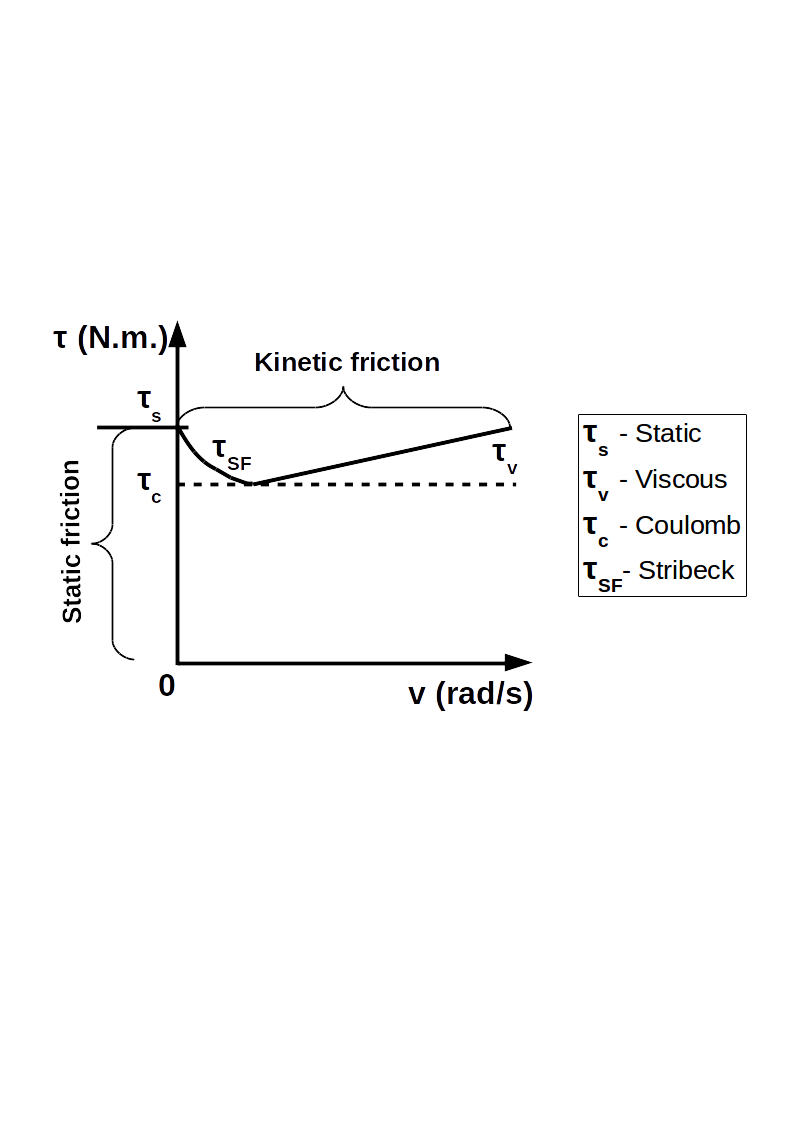
\includegraphics[width=100mm, trim=0 320 0 220]{pictures/friction_soa}
\caption{Friction model}
\end{figure}

The next important module of consideration in this work is the process control. PID controller is used by many of the standard industrial manipulators where each joint is attached with an independent PID. Mostly, single axis PID control scheme is used in the control applications~\cite{cascadedcontrol} and the controller gains can be tuned with different methods starting from empirical tuning (step-response based tuning)~\cite{astrom1995pid} to auto-tuning methods. The tracking accuracy of this method suffer in high-speed operations due the constraints in the mechanical systems. As discussed before, the manipulators are non-linear systems, it is important to account the complete dynamics of the system for the improved trajectory tracking~\cite{swevers}. There are different kinds of motion control methods available for the robot manipulators such as impedance control, computed-torque control which also has computed-torque like control~\cite{Chung2016}. Impedance control considers the interaction between the robot and the environment by accounting the dynamic characteristics of the system~\cite{de2012theory} rather than just doing force regulation based on the positions. In~\cite{muggler2013torque}, computed-torque control with the PD controller is put to work in the youBot manipulator along with dynamic model. The author has considered only the gravitational torques $\tau_g(q)$ in mathematical model and it does not account for torques due to friction. But this method needs accurate model parameters that can improve the overall result of the control scheme. It is important to consider the finding provided by the author~\cite{muggler2013torque} that the maximum applicable torque provided by the manufacturers are not sufficient to move the joints of the robot in some of the configurations of the manipulator. So, the author proposes a method that can compute the maximum applicable torque for the individual joints of the manipulator with the following equation~\eqref{eq:maxtorquemuggler}.

\begin{equation}
	\overbrace{\tau_{max}}^\text{nx1} = \overbrace{\textbf{M}_{max}}^\text{nxn} \overbrace{\textbf{K}_p}^\text{nxn} \overbrace{\textbf{e}_{max}}^\text{nx1}
\label{eq:maxtorquemuggler}
\end{equation}

where, $\tau_{max}$ represents the $n\times1$ matrix of torque that represents the maximum torque allowed in n joints of the manipulator and it is obtained by computing the product of the maximized manipulator inertia matrix, the proportional gain $K_p$ of the controller and the maximum possible joint position error $e_{max}$ and the error depends on the specifications of the particular joint. Input to the maximized manipulator inertia matrix is the joint positions where the manipulator joints are pushed to it's maximum in order to get the maximized inertia matrix. 

Chung~\cite{Chung2016} discusses computed-torque control scheme with the following formulation

\begin{equation}
\tau = H(q) \textit{v} + C(q,\dot{q})\dot{q} + \tau_g(q)
\end{equation} 

where computed torque-control consists of an inner non-linear compensation loop and the outer-loop with the control signal \textit{v}. This \textsl{control law is then substituted in the }dynamic model of the manipulator where $\ddot{q}_d$ is replaced with the control input \textit{v}. The substitution of this control law in the model solves a non-linear problem hence the linear control strategies can be applied. PD feedback control mechanism is used in the outer-loop control \textit{v}.  

\begin{equation}
\textit{v} = \ddot{q}_d + CV
\end{equation}

Computed-torque control described above is the proper control scheme and the author also provides a simple control scheme where the model and the controller works independent of each other (control input is not fed to model). Feed-forward and computed-torque control schemes discussed by~\cite{34773} results with reduction in the tracking error with the complete dynamics of the system. The model based controller requires accurate control on joint torque and it depends on the accuracy of joint position and velocity data. The computed torque-like control works by adding the variable compensation in the outer loop for accurate trajectory tracking~\cite{Chung2016} due to the uncertainties in the dynamic model. YouBot manipulator can be visualized in Simbody~\cite{sherman2011simbody} where the dynamics simulations can be achieved based on the recursive Newton-Euler formulation. Torque sensor can be created with the measured forces of gravity, bias and body forces, and it completes formulation of the generalized forces. Then the forces observed in the Cartesian space can be converted to joint torques. This library can be very useful in simulating the behaviour of the manipulator for the given motion control applications before testing it in the real robot.
\emptypage
%%%%%%%%%%%%%%%%%%%%%%%%%%%%%%%%%%%%%%%%%%%%%%%%%%%%%%%%%%%%%%%%%%%%%%%%%%%%%%%%%%%%%%%%%%%%%
%\chapter{PROBLEM STATEMENT} -- not always required the chapter name as problem statement.	%
% chapter problem statement - in this chapter the problem of the thesis are desribed.				%
%%%%%%%%%%%%%%%%%%%%%%%%%%%%%%%%%%%%%%%%%%%%%%%%%%%%%%%%%%%%%%%%%%%%%%%%%%%%%%%%%%%%%%%%%%%%%
\chapter{APPROACH}
\label{sec:approach}

This chapter discusses the detailed information about the approaches used in this work. At first, the basic approach depicted in Fig.~\ref{fig:basicapproach} is an advanced model based controller which gives the complete overview about all the components used in this work.

\begin{center}
\begin{tikzpicture}[auto, node distance=2cm,>=latex']
    \node [input, name=input] {};
    \node [sum, right of=input, node distance=1.5cm] (minus) {\textbf{-}};
    \node [block, right of=minus, node distance=2.1cm] (control) {\textbf{Controller}};
    \node [block, right of=control, node distance=3.5cm, pin={[pinstyle]above: $\psi$}] (model){\textbf{\shortstack{Dynamic\\ model}}};
    \node [sum, right of=model, node distance=2.5cm](summation) {\textbf{$\epsilon$}};
    \node [block, right of=summation,
            node distance=2.5cm] (robot) {\textbf{Robot}};
    \node [block, above of=robot, node distance=2cm](friction) {\textbf{\shortstack{Friction\\ observer}}};
	\node [output, right of=robot, node distance=2.9cm](output){};
	\draw [->,thick] (input) -- node {$q_d, \dot{q}_d$} (minus);
	\draw [->,thick] (minus) -- node {$e$} (control);
	\draw [->,thick] (control) -- node {$\ddot{q}_d$} (model);	
    \draw [->,thick] (model) -- node {$\tau$} (summation);
    \draw [->,thick] (summation) -- node {$\tau_m$} (robot);    
	\draw [->,thick] (friction) -- ++ (-2.0, 0) -| node [pos=-0.1] {$\tau_f$} (summation);	
    \draw [->,thick] (robot) -- node[pos=0.5] {$q_m, \dot{q}_m$} (output);
	\draw [->,thick] (output) -- ++ (0,-1.3) |- node [pos=0.7] {$\dot{q}_m$} (friction);
	\draw [->,thick] (output) -- ++ (0,-1.3) -| node [] {} (minus);
	\draw [->,thick] (output) -- ++ (0,-1.3) -| node [] {} (model);
\end{tikzpicture}
\captionof{figure}{Basic approach}
\label{fig:basicapproach}
\end{center}

The control scheme given above~\ref{fig:basicapproach} feeds the control variable as an acceleration $\ddot{q}_d$ input to the dynamic model for computing the model torques, whereas Chung et. al.~\cite{Chung2016} fed the actual desired acceleration $\ddot{q}_d$ as the model input in the defined control scheme. The reason for this difference in the controller scheme is that there is no accelerometer present in the manipulator joints. In such a case, it is only fair to answer the following question, why not differentiating the measured velocity to get the acceleration data?. The answer to the above question is that the measured velocity which is obtained from the encoders are generally noisy and taking the derivative of this data would amplify the noise much further, so the desired acceleration input is not considered in this work. An another important observation in this work is that the model considers only the link's moment of inertia and it can be subtracted from the motor's moment of inertia. The motor's moments of inertia can be computed with the specifications provided by the manufacturers. So, the alternate method is selected in this work for the model-based control as depicted in Fig.~\ref{fig:alternateapproach}. 

\begin{center}
\begin{tikzpicture}[auto, node distance=2cm,>=latex']
    \node [input, name=input] {};
    \node [input, above of=input, name=input1, node distance=1.5cm] {};
    \node [sum, right of=input, node distance=1.5cm] (minus) {\textbf{-}};
    \node [block, right of=minus, node distance=2.1cm] (control) {\textbf{Controller}};
    \node [block, above of=control, node distance=1.5cm, pin={[pinstyle]above: $\psi$}] (model){\textbf{\shortstack{Dynamic\\ model}}};
    \node [sum, right of=control, node distance=2.5cm](summation) {\textbf{$\epsilon$}};
    \node [block, right of=summation,
            node distance=2.5cm] (robot) {\textbf{Robot}};
	\node [output, right of=robot, node distance=2.9cm](output){};
	\draw [->,thick] (input) -- node {$q_d, \dot{q}_d$} (minus);
	\draw [->,thick] (input1) -- node {$\ddot{q}_d=0$} (model);
	\draw [->,thick] (minus) -- node {$e$} (control);
	\draw [->,thick] (control) -- node {$\tau_c$} (summation);	
    \draw [->,thick] (model) -| node {$\tau_{model}$} (summation);
    \draw [->,thick] (summation) -- node {$\tau_m$} (robot);    
    \draw [->,thick] (robot) -- node[pos=0.5] {$q_m, \dot{q}_m$} (output);
	\draw [->,thick] (output) -- ++ (0,-1.3) -| node [] {} (minus);
	\draw [->,thick] (output) -- ++ (0, 3.3) -| node [] {} (input1);
\end{tikzpicture}
\captionof{figure}{Alternative method - Computed torque-control which includes dynamic model}
\label{fig:alternateapproach}
\end{center}

The following components are really important to reach the ultimate goal of this project that is specified in Fig.~\ref{fig:alternateapproach}.

\begin{itemize}
\item \textbf{Robot/Process/Plant} represents the real system and it contains an actuator through which the process is controlled. The system that is used in this work is explained in detail in the preceding section. The disturbance in the system is the non-controlled variable that has an influence on the controller performance but the controller adjusts the control variable for compensating that influence. 
\item \textbf{Dynamic model} is required to generate the model torques based on Orocos KDL ID solver~\cite{smits2011kdl} and the manufacturer's 3D model~\cite{kukamanipulator} where $\psi$ represents the dynamic model parameters which can be replaced with the identified parameters once the estimation is successful. The friction compensation term $\tau_f$ is also considered in this work with the basic approach.
\item \textbf{Parameter estimation} that estimates the accurate model parameters. $\psi$ represents the dynamic model parameters. The excitation trajectories can be identified using the Finite Fourier series~\cite{SweversJ1997Orea} and the coefficients can be optimized for better identifying the model parameters. This section presents an overview about the parameter estimation and the trajectory parameterization and optimization.
\item \textbf{Controller} solves the control problem where it reduces the error by introducing the regulation in the system with the linear feedback control method. This work uses the cascade control mechanism and velocity of the joint is controlled in velocity PI controller. 
\end{itemize}

\newpage
\section{Description of the hardware platform}

This work uses the KUKA youBot for the implementation of the identification, control modules it comprises omnidirectional mobile platform and the manipulator. 

\subsection*{YouBot omnidirectional platform}

The base of the robot has 4 omnidirectional wheels with the separate motors attached to each of the wheel joints. It is particularly useful in testing the controller before performing the test in the manipulator where the joint limits are applicable. 

\begin{figure}[h]
\centering
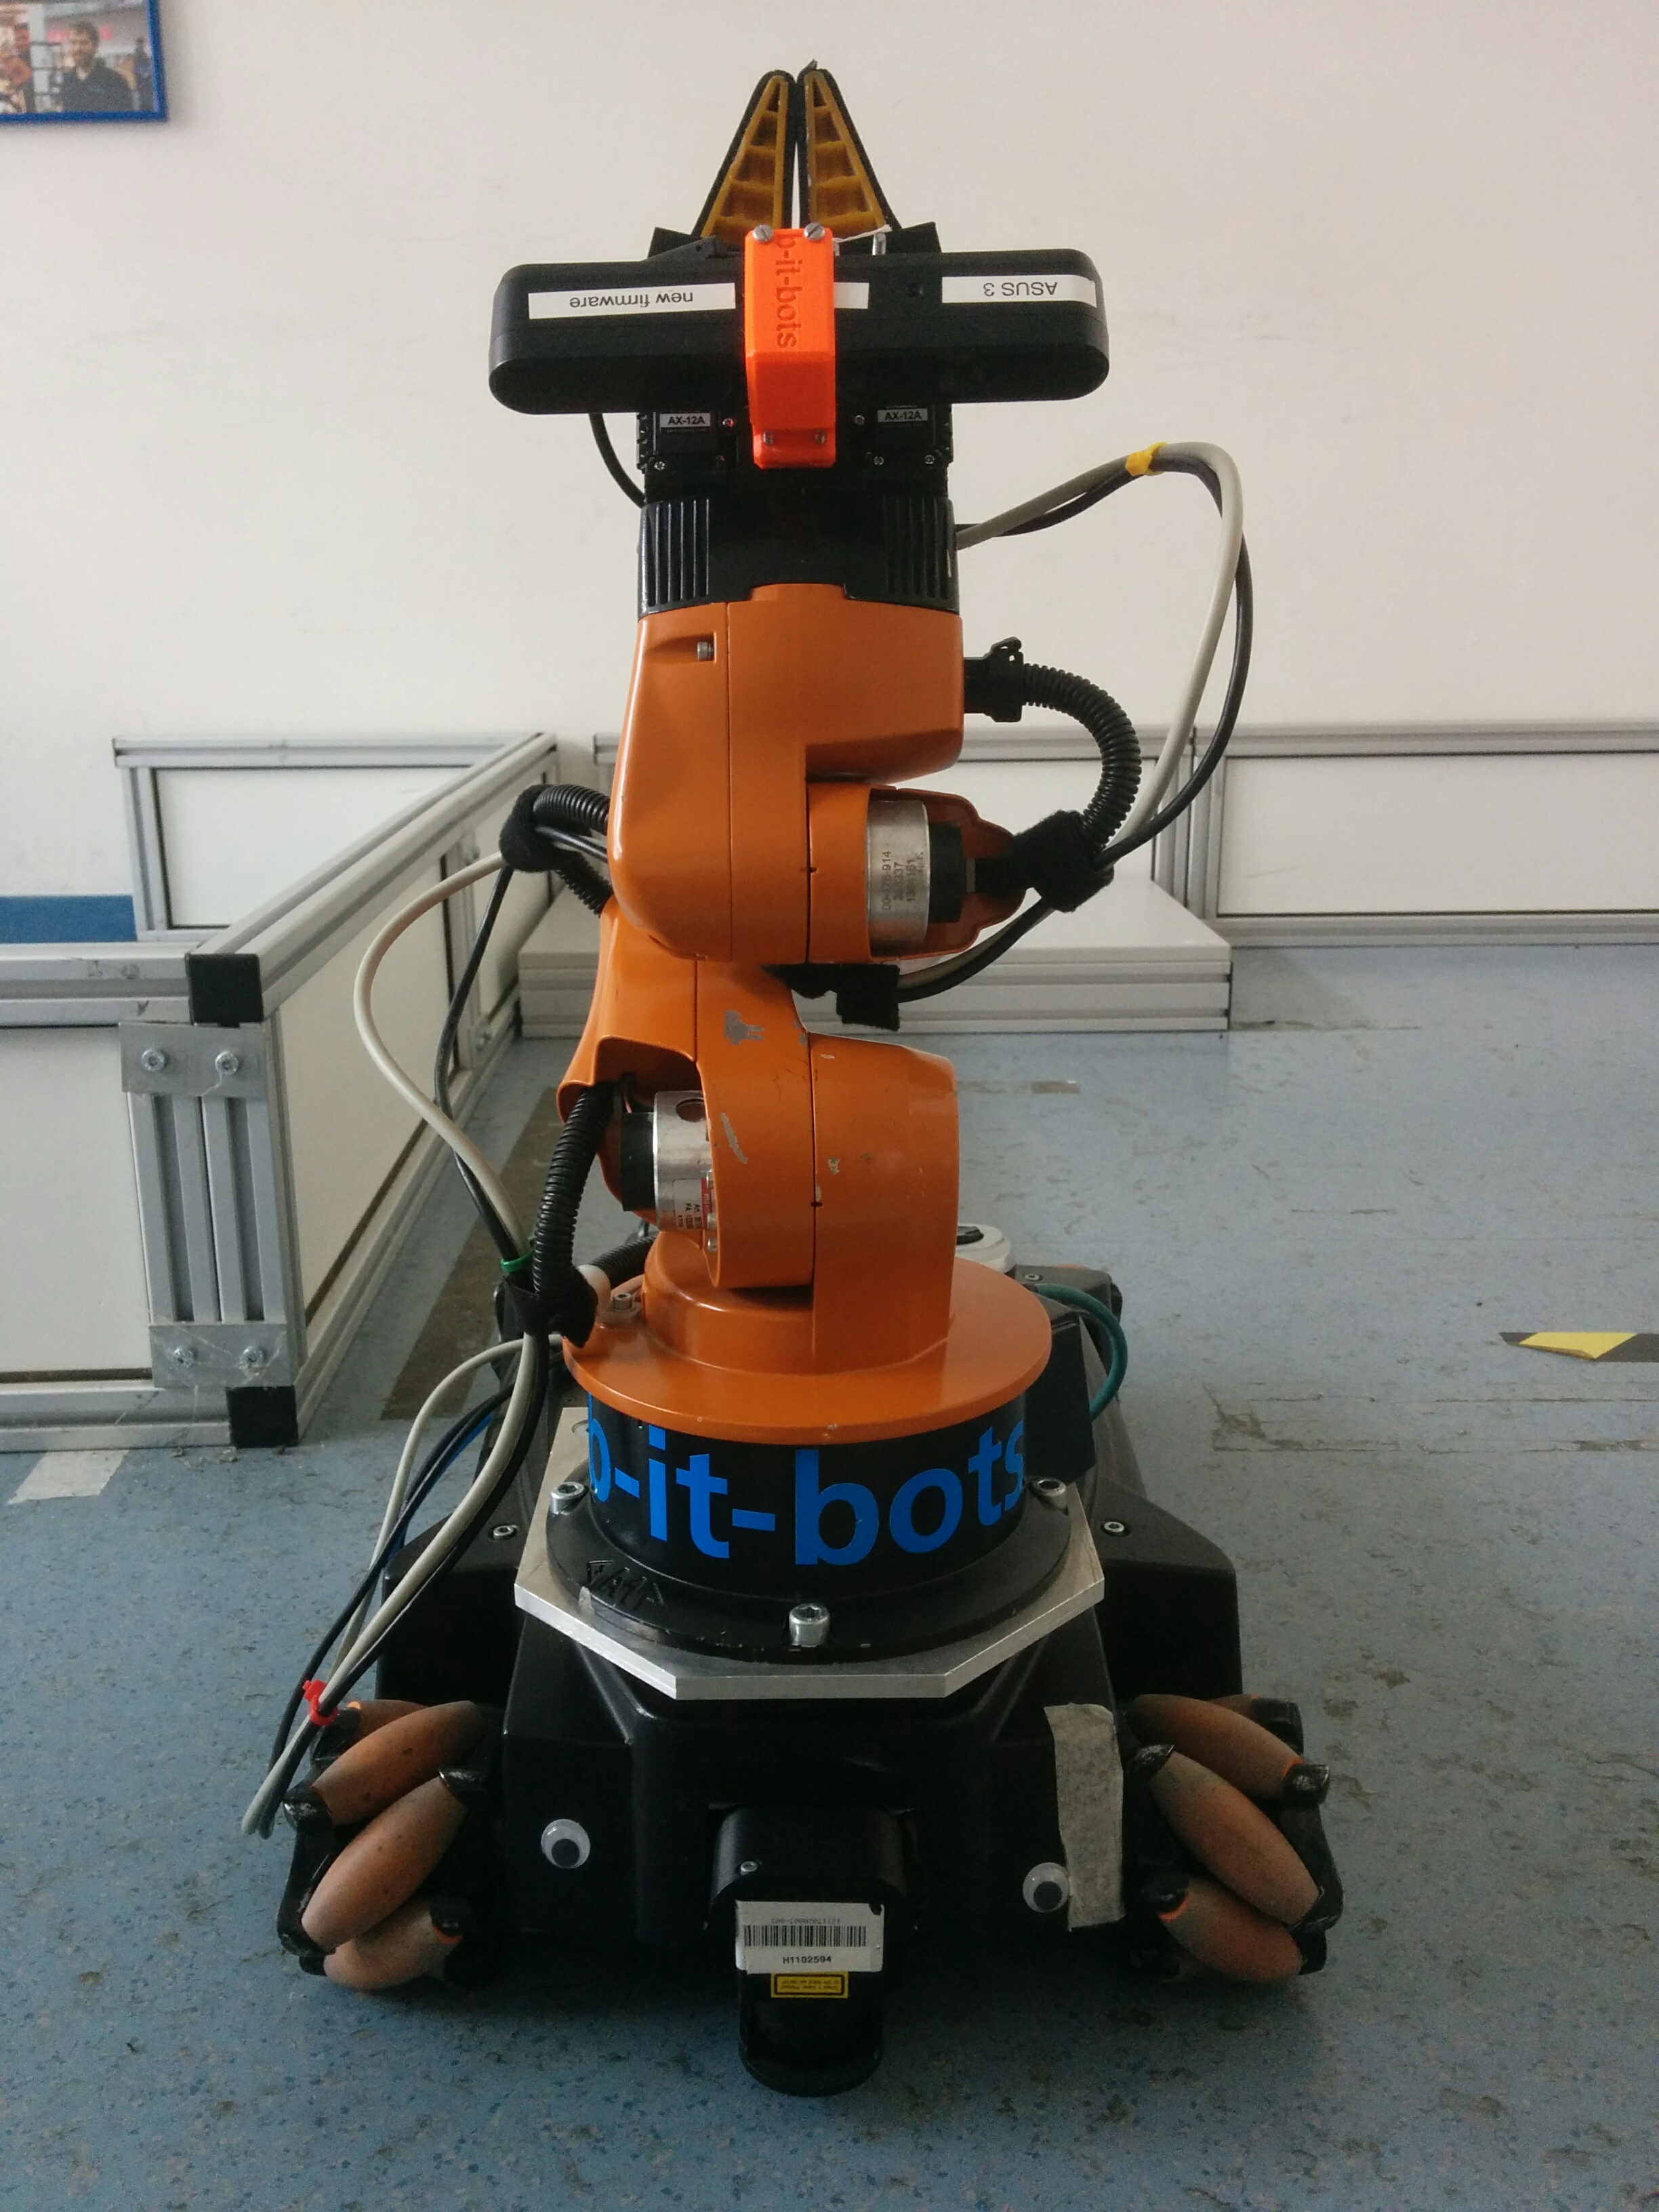
\includegraphics[width=60mm, trim=0 50 0 20]{pictures/youbot.jpg}
\caption[base]{youBot platform and manipulator}
\end{figure}

\subsection*{YouBot manipulator}

The main focus of this work is to achieve the computed-torque control in the youBot manipulator. The youBot arm consists of five rotary joints with 5-DoF controlled by the individual motors and it includes gripper in the last link which has two fingers. But this work does not consider the gripper both in modelling and the torque computation. The manipulator joints are commanded with the position or velocity or torque inputs through EtherCAT which has a real-time capability. The 3-D model of the manipulator is provided by the manufacturer~\cite{kukamanipulator} and it is used for modelling purposes and it is also used in computed-torque control where the model torques are computed. In order to increase the tracking performance, the gain values are tuned to a high value where there is a possibility of the overshoot problem. Due to this, the joint might cross the limits provided by the manufacturers hence it is important to introduce an artificial position limits to the joints for avoiding any damages to the system. The introduction of the limiting features and the safety controller is explained in the proceeding sections. Since the joints are commanded in torque mode, it is necessary to verify the maximum applicable torque for the individual joints of the manipulator. By considering the specifications provided by the manufacturers, the maximum applicable joint torques were identified with the following equation~\eqref{eq:maximumtorque}

\begin{equation}
\tau_{max} = \tau_{nominal} \cdot gear\_reduction\_ratio
\label{eq:maximumtorque}
\end{equation}

where nominal torque is represented in N.m., and gearbox reduction ratio values are referred from youBot-store's detailed specifications\footnote{\url{http://www.youbot-store.com/wiki/index.php/YouBot_Detailed_Specifications}}. The computed maximum joint torques are listed in the following table 3.1

% Please add the following required packages to your document preamble:
% \usepackage{multirow}
\begin{table}[h]
\begin{tabular}{|l|l|l|l|l|l|}
\hline
\multirow{2}{*}{\textbf{3-D Model}} & \textbf{Joint1} & \textbf{Joint2} & \textbf{Joint 3} & \textbf{Joint 4} & \multicolumn{1}{c|}{\textbf{Joint5}} \\ \cline{2-6} 
                                    & \multicolumn{5}{c|}{\textbf{In Newton meters (N.m.)}}                                                           \\ \hline
Existing $\tau_{max}$                     & 9.500           & 9.500           & 6.000            & 2.000            & 1.000                                \\ \hline
New $\tau_{max}$                      & 12.901          & 12.901          & 8.270            & 4.175            & 1.755                                \\ \hline
\end{tabular}
\caption{The maximum applicable joint torques provided by the manufacturers and it is computed from the equation~\eqref{eq:maximumtorque}}
\end{table}

The youBot-store specifications does not clearly state the nominal torque of the joint 5 hence the motor details are referred from~\cite{corberan2012haptic} which has the specifications of 15Watt brushless Maxon EC32 flat motor with the Hal sensor number 267121\footnote{\url{https://www.maxonmotor.com/medias/sys_master/root/8825434800158/17-EN-262.pdf}}.

\newpage
\section{Description of the software platform}

This section briefly discusses the software and libraries used in this work such as the youBot driver~\cite{youbotdriver}, Orocos KDL~\cite{smits2011kdl} and Simbody~\cite{sherman2011simbody}. All the software used in this work is developed in Ubuntu 14.04 operating system.

\subsection*{YouBot driver}

The youBot base and manipulator can be controlled via youBot-driver~\cite{youbotdriver} and the cmake version of the driver is used in this work. The communication with the robotic joints can be established via EtherCAT master~\cite{youbotdriver} which runs in a frequency of 1KHz (1 ms) hence a delay of 1 ms is introduced in computed-torque controller that is implemented in this work. The youBot-driver's architecture overview is given in Fig.~\ref{fig:youbotdriverarchitecture}. 

\begin{figure}[h]
\centering
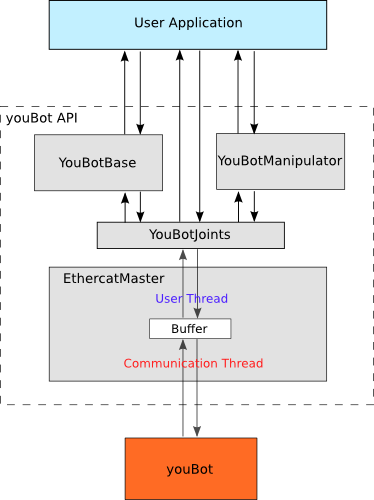
\includegraphics[width=60mm, trim=0 0 0 0]{pictures/youbotdriver_architecture}
\caption{youBot driver architecture overview and the image is taken from~\cite{youbotdriver_architecture}}
\label{fig:youbotdriverarchitecture}
\end{figure}

\subsection*{Simbody}

Simbody\footnote{\url{https://simbody.github.io/simbody-3.6-doxygen/api/index.html}}~\cite{sherman2011simbody} is the simulation engine that is used in this work to simulate and visualize youBot manipulator. Simbody follows recursive equations of motion similar to Featherstone~\cite{featherstone2014rigid} for the n joint DoF. It is a part of the simulation toolkit named SimTK which is an interface that gives access to the physics based simulation features. It is possible to perform the internal coordinate simulations of the multi-body systems by using Simbody API\footnote{\url{https://simtk.org/docman/?group_id=47}}. The multi-body system can be seen as the combination of rigid bodies that are connected through joints. Semantics of a rigid-body is given in Fig.~\ref{fig:simbody_rigidbody}. Simbody comprises two important classes which are related to the multi-body system such as system and state. The system class provides access to the logic for simulation which is constant and the state information stores the data overtime. 

\begin{figure}[h]
\centering
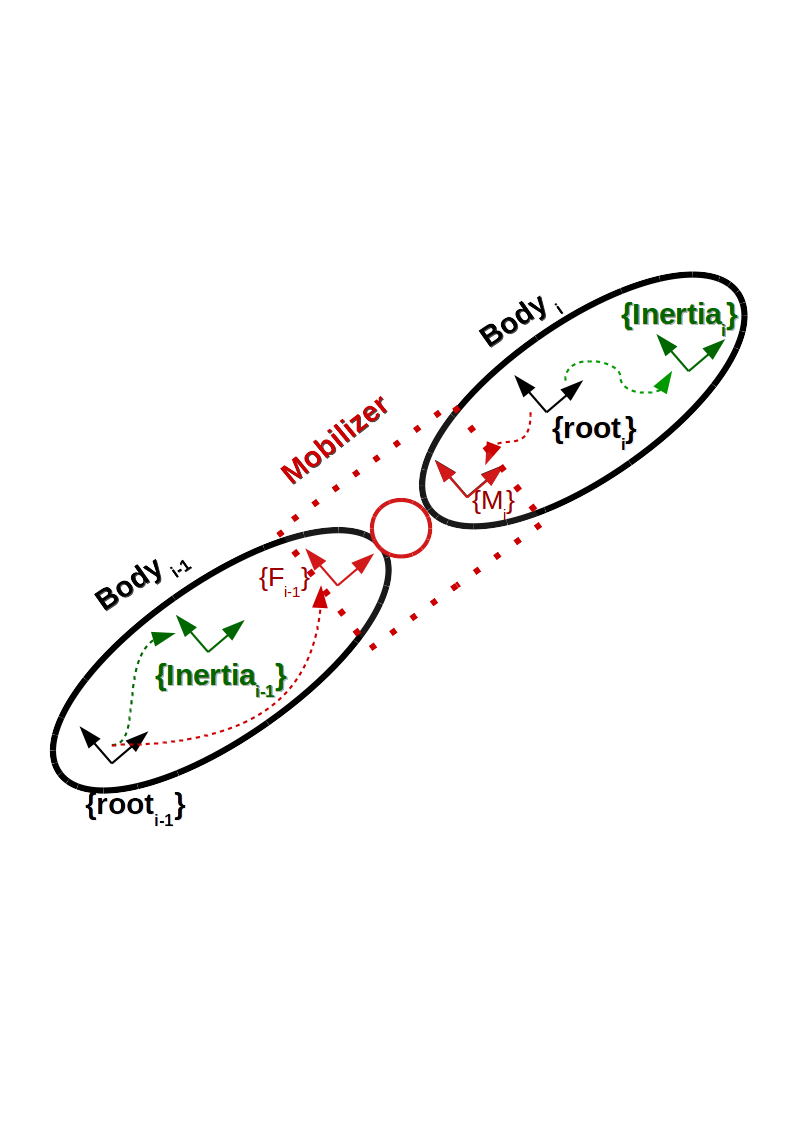
\includegraphics[width=80mm, trim=0 200 0 200]{pictures/simbody_rigidbody}
\caption{Rigid body semantics in SimTK}
\label{fig:simbody_rigidbody}
\end{figure}

In Simbody, MobilizedBody represents the basic body and joint object which is added to the multibody tree. The MobilizedBody connects the child to the existing parent body which is assumed to be ground with the use of the mobilizer and also assigns the reference frame to the parent body. The mobilizer has two frames attached with it such as the fixed frame F is attached to the parent body which is the reference to account the motion of the moving frame M of the child body respectively. The Pin joint is used in this work as manipulator joints are revolute joints where the axis of rotation is possible around only one axis. The above figure describes the mobility of the child body ($body_{i}$) with respect to the reference $body_{i-1}$ with the use of the coordinate frames. Simbody considers that the parent ($body_{i-1}$) is attached to the ground and the $body_i$ is the child body that does all the motions. The root frames of the rigid bodies i-1 and i are represented as $root_{i-1}, root_i$ respectively. The transformation from the body i to body i-1 can be given as

\begin{equation}
^{root_{i-1}}T_{root_i} = ^{root_{i-1}}T_{F_{i-1}}\cdot ^{F_{i-1}}T_{M_i}\cdot ^{M_i}T_{root_i}
\end{equation}

The mobilizer transformation from $M_i$ to $F_{i-1}$ mainly depends on the joint's coordinate $^{F_i}T_{M_i}$ which helps to locate the relative pose of the coordinate frame M with respect to the frame F. The other two segment transforms of both the parent and child body are composed with the mobilizer transform gives us the relative pose of the child body with respect to its parent. 

Before getting into further details, the following changes are made in the construction of the youBot manipulator in the visualizer. The pose of the CoM vector is represented w.r.t. the body's reference frame and the moments of inertia is in the principle axis. It is very clear from the Fig.~\ref{fig:simbody_rigidbody} that the inertial frame is represented with respect to the body's reference frame. But the kinematic chain for the 3-D model has a convention that the body's reference frame is coinciding with the joint reference frame. Hence, the second transformation in the joint description is an identity. In order to adapt to the convention used by Simbody, the inertial frame has to be re-expressed and shifted. Simbody provide sufficient methods to re-express and shift the inertia and the implementation details are discussed in appendix~\ref{sec:appendixC}. Torque sensor is built in Simbody for getting the torques from the manipulator joints, it gives the way to get the external forces such as bias, gravity forces and the mapping of the Cartesian forces into joint torque by using inverse Jacobian. Since the same 3-D model is used in Orocos-KDL, the offset computation is carried out to match the input joint positions with respect to the model. The joint positions are then fed to the Simbody where the inverse of the KDL offset computation is fed to Simbody since the same model is used and it takes raw youBot configuration as an input. Note that the result of the Simbody joint position measurements are inverted back to youBot's raw data since the joint position feedback is given back to KDL based ID solver. The Simbody's convention is semantically mismatching with KDL based ID solver in the implementation. The mismatch is observed when applying model torques that are computed using KDL to the manipulator joints in Simbody for the purpose of gravity compensation task. The result of this task is that the gravity compensation terms in youBot manipulator joints are accounted but the joints are slowly drifting away from the candle configuration overtime in further iterations of the visualizer. 

\newpage
\subsection*{Orocos KDL}

An important requirement for the model-based controller is to have a mathematical model that can predict the torque which is close-enough to the real system. A model comprises the physical properties of the robot such as kinematic, geometric and dynamic properties which are particularly useful in computing the model torques based on the given trajectory information. For this purpose, an open source library called Orocos KDL~\cite{smits2011kdl} is selected with an intend of modelling, computing the kinematic chain and predict torques using the recursive Newton-Euler ID (Inverse Dynamics) solver. The kinematic chain of the robot comprises segments of the manipulator itself and each segment has both the link and the joints attached between the links. The joint axis is negative for the joint number 5 hence the torque and velocity of the joint 5 has be inverted before commanding the model torques to the real robot.

\begin{figure}[h]
\centering
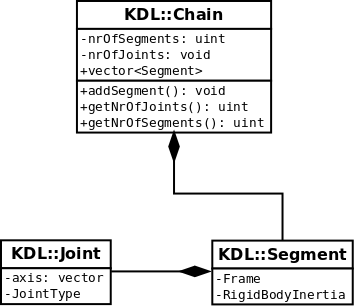
\includegraphics[width=75mm, trim=0 0 0 0]{pictures/kdlchain_classdiagram}
\caption{Kinematic chain in Orocos KDL which is a combination of both the joint and link}
\label{fig:kdlchain}
\end{figure}

The kinematic chain (KDL::Chain) of the robot is the collection of segments (KDL::Segment $0\cdot \cdot \cdot total number of segments$) where the segment is the combination of the link and joint (KDL::Joint) properties as depicted in Fig.~\ref{fig:kdlchain}. The implementation details are discussed briefly in appendix~\hyperref[sec:appendixB]{B}. 

\begin{center}
\begin{tikzpicture}[scale =1.8, tdplot_main_coords, -stealth]
\tdplotsetrotatedcoords{0}{0}{170}
\draw[red] (0,0,0) -- (1,0,0) node[anchor=north east]{$x$};
\draw[blue] (0,0,0) -- (0,1,0) node[anchor=north west]{$y$};
\draw[black] (0,0,0) -- (0,0,1) node[anchor=south]{$z$};
\coordinate (Shift) at (0,0,2.5);
\tdplotsetrotatedcoordsorigin{(Shift)}
\node [label={[xshift=5.0cm,yshift=0.5cm]base}]{};
\node [label={[xshift=5.0cm,yshift=3.4cm]Joint 1}]{};
\node [label={[xshift=5.0cm,yshift=6.9cm]Joint 2}]{};
\node [label={[xshift=5.0cm,yshift=10.5cm]Joint 3}]{};
\node [label={[xshift=5.0cm,yshift=14cm]Joint 4}]{};
\node [label={[xshift=5.0cm,yshift=17cm]Joint 5}]{};
\tdplotdrawarc[->,color=black]{(-0.75,2.1,0)}{0.1}{160}{330}{anchor=south east,color=black}{}
\coordinate (Origin) at (0,0);

\draw[thin, dashed] [->] (Origin)  arc (3.2:36.9:11.8) node [right,pos=1.5] {};
\tdplotsetrotatedcoords{-90}{-180}{90}
\draw[color=red,tdplot_rotated_coords,->] (0,0,0)
-- (1,0,0) node[anchor=south east]{$x$};
\draw[color=blue,tdplot_rotated_coords,->] (0,0,0)
-- (0,1,0) node[anchor=west]{$y$};
\draw[color=black,tdplot_rotated_coords,->] (0,0,0)
-- (0,0,1) node[anchor=south]{$z$};
\node [label={[xshift=2.4cm,yshift=2.3cm]\tiny\tiny \textbf{Relative Pose}}]{};
\node [label={[xshift=2.7cm,yshift=2cm]\tiny\tiny(X Y Z = 0.024m 0m 0.115m)}]{};
\node [label={[xshift=2.27cm,yshift=1.7cm]\tiny\tiny(Z Y X = 0$^{\circ}$ 0$^{\circ}$ 180$^{\circ}$)}]{};\tdplotdrawarc[->,color=black]{(-0.78,2.1,1)}{0.1}{90}{-90}{anchor=south east,color=black}{}

\coordinate (Shift) at (0,0,4);
\tdplotsetrotatedcoordsorigin{(Shift)}
\tdplotsetrotatedcoords{-90}{-90}{0}

\draw[thin, dashed] [->] (Origin)+(-2.35,6.45)  arc (3.2:36.9:7.1) node [right,pos=0.5] {};

\draw[color=red,tdplot_rotated_coords,->] (0,0,0)
-- (1,0,0) node[anchor=south east]{$x$};
\draw[color=blue,tdplot_rotated_coords,->] (0,0,0)
-- (0,1,0) node[anchor=west]{$y$};
\draw[color=black,tdplot_rotated_coords,->] (0,0,0)
-- (0,0,1) node[anchor=south]{$z$};
\node [label={[xshift=2.3cm,yshift=5.3cm]\tiny\tiny \textbf{Relative Pose}}]{};
\node [label={[xshift=2.45cm,yshift=5cm]\tiny\tiny(X Y Z = 0.033m 0.0m 0.0m)}]{};
\node [label={[xshift=2.12cm,yshift=4.7cm]\tiny(Z Y X = -90$^{\circ}$ 0$^{\circ}$ 90$^{\circ}$)}]{};
\tdplotdrawarc[->,color=black]{(-0.08,0.9,3.9)}{0.1}{-240}{80}{anchor=south west,color=black}{}

\coordinate (Shift) at (0,0,6);
\tdplotsetrotatedcoordsorigin{(Shift)}
\tdplotsetrotatedcoords{-90}{-90}{-90}
\draw[thin, dashed] [->] (Origin)+(-3.8,10.6)  arc (4.1:36.9:9.2) node [right,pos=0.5] {};
\draw[color=red,tdplot_rotated_coords,->] (0,0,0)
-- (1,0,0) node[anchor=south east]{$x$};
\draw[color=blue,tdplot_rotated_coords,->] (0,0,0)
-- (0,1,0) node[anchor=west]{$y$};
\draw[color=black,tdplot_rotated_coords,->] (0,0,0)
-- (0,0,1) node[anchor=south]{$z$};
\node [label={[xshift=2.3cm,yshift=8.5cm]\tiny\tiny \textbf{Relative Pose}}]{};
\node [label={[xshift=2.5cm,yshift=8.2cm]\tiny\tiny(X Y Z = 0.155m 0.0m 0.0m)}]{};
\node [label={[xshift=2.1cm,yshift=7.9cm]\tiny(Z Y X = -90$^{\circ}$ 0$^{\circ}$ 0$^{\circ}$)}]{};
\tdplotdrawarc[->,color=black]{(-0.08,0.9,5.9)}{0.1}{240}{-90}{anchor=south west,color=black}{}

\coordinate (Shift) at (0,0,8);
\tdplotsetrotatedcoordsorigin{(Shift)}
\tdplotsetrotatedcoords{-90}{-90}{-90}
\draw[thin, dashed] [->] (Origin)+(-5.65,15.6)  arc (4.2:36.4:9.75) node [right,pos=0.5] {};
\draw[color=red,tdplot_rotated_coords,->] (0,0,0)
-- (1,0,0) node[anchor=south east]{$x$};
\draw[color=blue,tdplot_rotated_coords,->] (0,0,0)
-- (0,1,0) node[anchor=west]{$y$};
\draw[color=black,tdplot_rotated_coords,->] (0,0,0)
-- (0,0,1) node[anchor=south]{$z$};
\node [label={[xshift=2.4cm,yshift=12cm]\tiny\tiny \textbf{Relative Pose}}]{};
\node [label={[xshift=2.5cm,yshift=11.7cm]\tiny\tiny(X Y Z = 0.0m 0.135m 0.0m)}]{};
\node [label={[xshift=1.97cm,yshift=11.4cm]\tiny(Z Y X = 0$^{\circ}$ 0$^{\circ}$ 0$^{\circ}$)}]{};
\tdplotdrawarc[->,color=black]{(-0.08,0.9,7.9)}{0.1}{-240}{80}{anchor=south west,color=black}{}

\coordinate (Shift) at (0,0,10);
\tdplotsetrotatedcoordsorigin{(Shift)}
\tdplotsetrotatedcoords{-90}{0}{-90}
\draw[thin, dashed] [->] (Origin)+(-7.55,21)  arc (4.8:37.1:9.3) node [right,pos=0.5] {};
\draw[color=red,tdplot_rotated_coords,->] (0,0,0)
-- (1,0,0) node[anchor=south east]{$x$};
\draw[color=blue,tdplot_rotated_coords,->] (0,0,0)
-- (0,1,0) node[anchor=west]{$y$};
\draw[color=black,tdplot_rotated_coords,->] (0,0,0)
-- (0,0,1) node[anchor=south]{$z$};
\node [label={[xshift=2.45cm,yshift=15.5cm]\tiny\tiny \textbf{Relative Pose}}]{};
\node [label={[xshift=2.55cm,yshift=15.2cm]\tiny\tiny(X Y Z = 0.0m 0.1136m 0.0m)}]{};
\node [label={[xshift=2.1cm,yshift=14.9cm]\tiny(Z Y X = 0$^{\circ}$ 0$^{\circ}$ -90$^{\circ}$)}]{};
\tdplotdrawarc[->,color=black]{(-0.5,1.5,10.1)}{0.1}{0}{280}{anchor=south west,color=black}{}
\end{tikzpicture}
\captionof{figure}{Frame representation of the youBot-store 3-D model based on ~\cite{kukamanipulator} and image is taken from~\cite{RnD2Rajagopal}}
\end{center}

\newpage
The raw joint angles of the youBot can't be used in kinematic and dynamic computations in KDL since the model has a different coordinate system representation comparing the real robot. So, it is important to compute the offsets for the model w.r.t. the youBot coordinate system i.e. by default, the youBot manipulator is present in the minimum configuration in the real system but 3-D model represents candle configuration as the minimum configuration hence offset calculation is needed to represent the joint information properly in KDL before inputting the joint positions to the forward position kinematics, torque computations.

% Please add the following required packages to your document preamble:
% \usepackage{multirow}
\begin{table}[h]
\begin{tabular}{|l|l|l|l|l|l|l|l|l|l|}
\hline
\multicolumn{2}{|l|}{\multirow{2}{*}{\textbf{\begin{tabular}[c]{@{}l@{}}Joint \\ No.\end{tabular}}}} & \multicolumn{4}{l|}{\textbf{youBot raw values(in Radians)}}               & \multicolumn{4}{l|}{\textbf{\begin{tabular}[c]{@{}l@{}}youBot-store 3D model \\ (in Radians)\end{tabular}}} \\ \cline{3-10} 
\multicolumn{2}{|l|}{}                                                                               & \textbf{Min} & \textbf{Max} & \textbf{Candle} & \textbf{Folded} & \textbf{Min}            & \textbf{Max}            & \textbf{Candle}            & \textbf{Folded}            \\ \hline
\multicolumn{2}{|l|}{1}                                                                              & 0.0          & 5.8992       & 2.9496          & 0.0             & -2.9496                 & 2.9496                  & 0.0                        & -2.9496                    \\ \hline
\multicolumn{2}{|l|}{2}                                                                              & 0.0          & 2.7053       & 1.1345          & 0.0             & -1.1345                 & 1.1345                  & 0.0                        & -1.1345                    \\ \hline
\multicolumn{2}{|l|}{3}                                                                              & -5.1836      & 0.0          & -2.5482         & 0.0             & -2.6354                 & 2.5482                  & 0.0                        & 2.5482                     \\ \hline
\multicolumn{2}{|l|}{4}                                                                              & 0.0          & 3.5779       & 1.7890          & 0.0             & -1.7890                 & 1.7890                  & 0.0                        & -1.7890                    \\ \hline
\multicolumn{2}{|l|}{5}                                                                              & 0.0          & 5.8469       & 2.9234          & 0.0             & -2.9234                 & 2.9234                  & 0.0                        & -2.9234                    \\ \hline
\end{tabular}
\end{table}

It is important to consider the correctness of the frame diagram provided by KDL library before jumping into the implementation of the same. This work has an important finding with KDL's frame diagram and it is explained in detail as follows

\begin{figure}[h]
\centering     %%% not \center
\subfigure[KDL segment, image from kinematic-trees section of the kdl user-manual~\cite{smits2011kdl}]{\label{fig:a}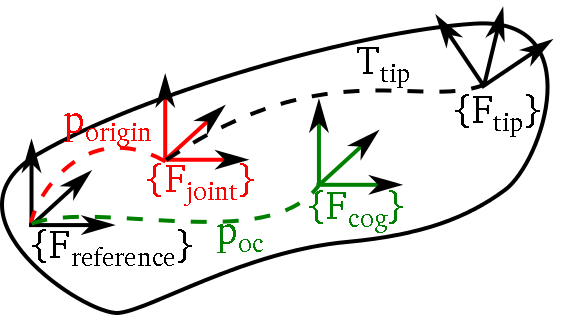
\includegraphics[width=60mm]{pictures/kdl_segment}}
\subfigure[Modified KDL segment]{\label{fig:b}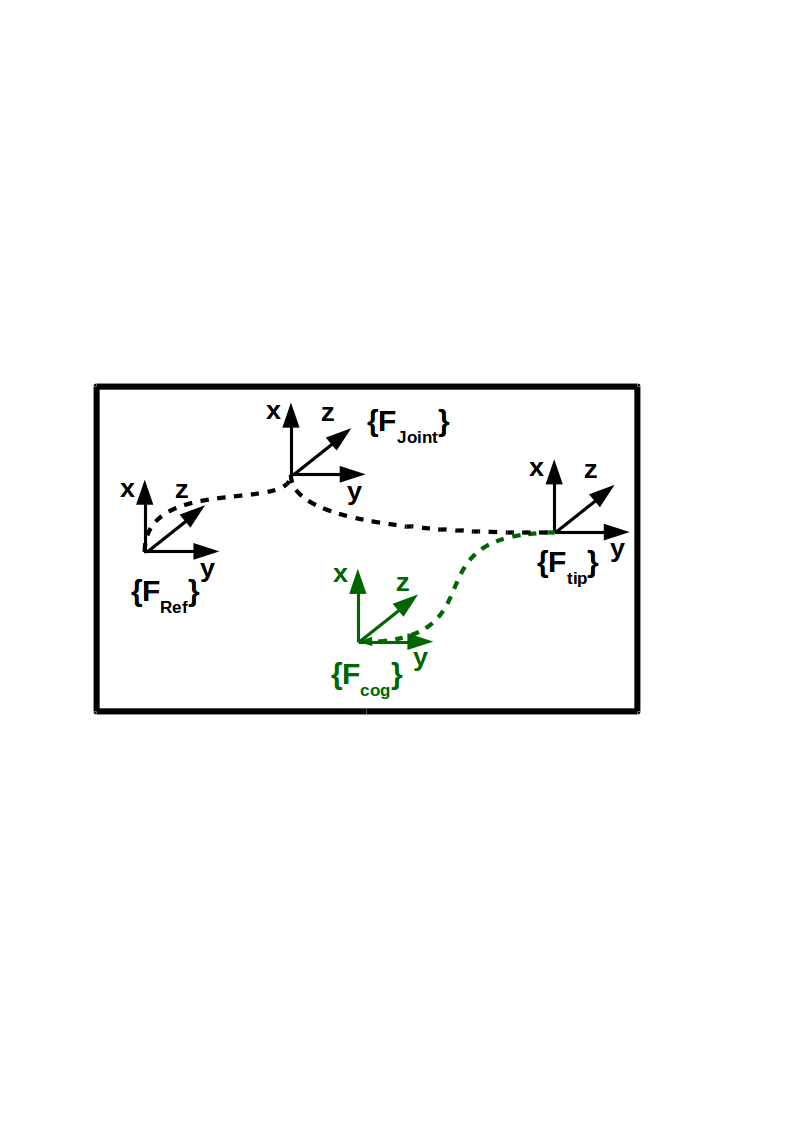
\includegraphics[trim=0 300 0 250, width=75mm]{pictures/KDL_segment_modified}}
\caption{Correction in KDL frame diagram}
\end{figure}

The sample application is created to check whether the inertia is being felt in the reference frame or the tip frame of the segment. Consider an example where the tip of segment is translated by [0.5, 0.0, 0.0] (in meters) from the joint by 0.5 meters in x-axis and the CoM can be located by the vector [x = 0.5, y = 0.0, z = 0.0] (in meters) from the reference frame of the body. Where the result of this experiment is -9.81 Nm due to the lever arm of the tip frame and the CoM vector. According to this experiment, it is proven that the CoM vector is not located w.r.t. the reference frame of the body rather it is defined w.r.t. the tip frame. So, it is mandatory to represent the CoM vector w.r.t. the reference frame as per the convention used by the youBot-store's 3D model. This transformation can be easily done by multiplying the inverse of the transform from $^{tip}X_{joint}$ (the relative pose from the reference frame to tip frame) with the CoM vector.

The convention used in KDL is different from the conventions in youbot-store model~\cite{kukamanipulator}. For example, the following Fig.~\ref{fig:a1} depicts the convention used by Orocos KDL library and the orientation of the inertial frame is same as the reference or joint frame. This means that inertial frame is just translated w.r.t. the segment's reference frame. On the other hand, youbot-store model uses the convention where the inertial frame is both translated by $P_{oc}$ vector and oriented differently by Z-Y-X angle. This work considers that both the segment's reference and joint frames are the same.

\begin{figure}[h]
\centering
\subfigure[KDL segment, image from kinematic-trees section of the kdl user-manual~\cite{smits2011kdl}]{\label{fig:a1}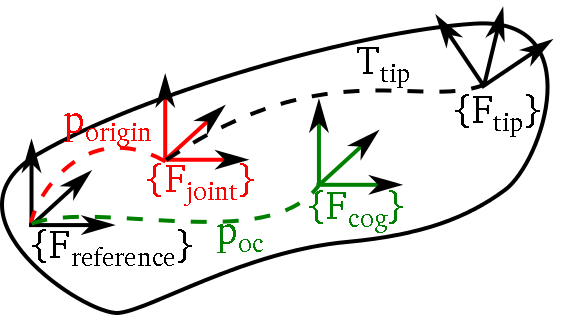
\includegraphics[width=60mm]{pictures/kdl_segment}}
\subfigure[Youbot-store segment]{\label{fig:b1}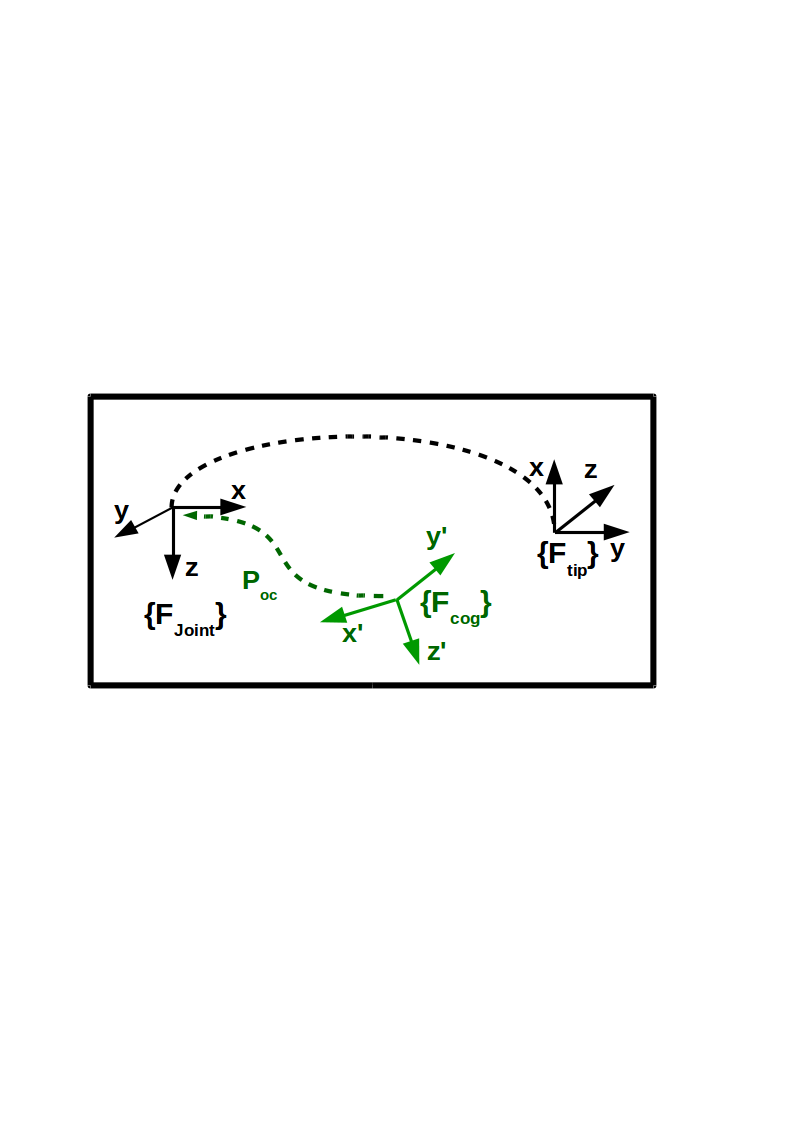
\includegraphics[trim=0 300 0 250, width=75mm]{pictures/store_segment}}
\caption{Different conventions used by kdl and youBot-store}
\end{figure}

Based on the finding given above, if the developer wants to use the KDL library for kinematic and dynamic computations then the convention of the 3-D model has to be the same as KDL representation i.e, this work uses the youbot-store model to compute model torques hence the convention is changed according to KDL's convention as follows. The orientation of the inertial frame in the youBot-store model is not matching up with the convention used in KDL. So, the following equation~\eqref{eqn:jointinertiaorientationchange} can be used to align the orientation of the inertial frame w.r.t. the orientation of the joint reference frame.

\begin{equation}
I_{\{Joint\}} = R^T \cdot I_{\{cog\}} \cdot R
\label{eqn:jointinertiaorientationchange}
\end{equation}

where I$_{\{Joint\}}$, I$_{\{cog\}}$ represents the rigid body inertia with respect to the joint frame, center of gravity respectively and the rotation matrix that is used as the reference orientation R is taken from the joint frame. 

\section{Semantics for rigid-body algorithms}

The definitions and the conventions of this section are written based on the reference from articles~\cite{geometicsemanticspart1}~\cite{geometicsemanticspart2}. An important characteristics of the manipulation involves the analysis of the motion of the rigid bodies in three dimensional space and the rigid body which can't deform is considered in this work. Each and every rigid-body has 6-DoF (3-DoF each for the rotation and translation) in space where there are no constraints present. Basically, a constraint refers to the joint when it is attached to the rigid body, only 1-DoF exists. The geometrical relations between the rigid bodies such as position, orientation, pose, linear, angular velocity and twist, forces, torques and wrenches are important for the rigid-body algorithm. The pose, relative motion and the relative effort transmission between the rigid bodies must be represented in a very well defined coordinate system. If the developer fails to choose the coordinate system carefully it might lead to the logical errors that are difficult to trace. The coordinate system representations are mostly implicitly defined by the libraries such as Simbody~\cite{sherman2011simbody}, KDL~\cite{smits2011kdl} and the authors define their own representations which are semantically correct. So, it is important to decode the implicit conventions in order to avoid the logical errors in the geometrical relation semantics representation of the rigid bodies. For example, the following diagram shows different conventions used by two different authors hence the homogeneous transformation matrix that is useful in finding the relative pose between the two frames changes the coordinate calculations accordingly.

\begin{figure} [H]
\centering     %%% not \center
\subfigure[JJ. Craig]{\label{fig:craigconvention}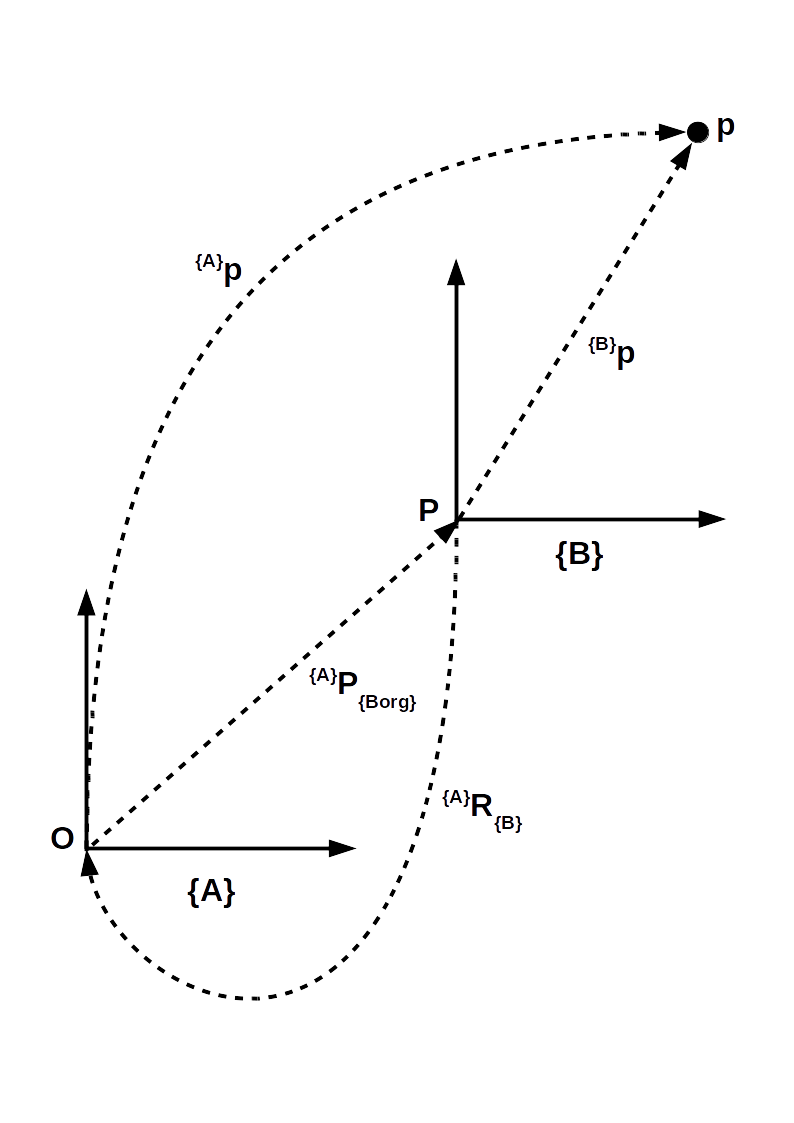
\includegraphics[width=70mm]{pictures/jjcraig_motionandwrenchtransmission.png}}
\subfigure[Featherstone]{\label{fig:featherstoneconvention}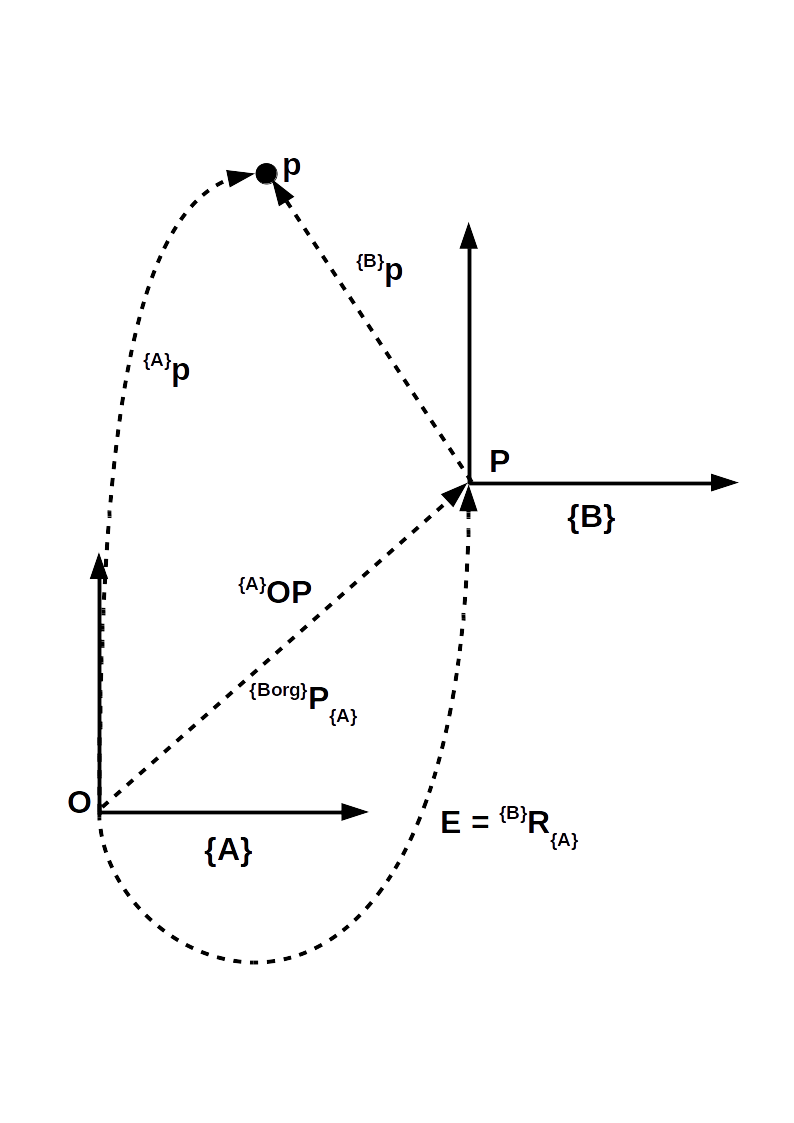
\includegraphics[width=70mm]{pictures/featherstone_motionandwrenchtransmission.png}}
\caption{Different conventions used by different authors~\cite{featherstone2014rigid}~\cite{craig2005introduction}.}
\label{fig:diffinconventions}
\end{figure}

The inverse of the transform can be computed numerically with the following equations. 

\begin{align*}
	& \textbf{JJ Craig}&&\textbf{Featherstone} \\
    & ^{{A}}P = ^{{A}}_{{B}}R \cdot ^{{B}}P + ^{A}P_{Borg}&&^{{B}}P = ^{{B}}_{{A}}R^{T} \cdot ^{A}P^{-1}_{Borg} + ^{A}P\nonumber \\ \\
    & && ^{B}P = ^{B}_{A}R\cdot ^{A}P - ^{B}_{A}R\cdot ^{A}P_{Borg} \\ \\
    & && ^{B}P = ^{B}_{A}R\cdot (^{A}P - ^{A}P_{Borg}) \\ \\
    & ^{A}_{B}T = \begin{bmatrix}
    				^{{A}}_{{B}}R & P_{Borg} \\
    				\textbf{0} & 1
				  \end{bmatrix} && ^{B}_{A}T = \begin{bmatrix}
    				^{{B}}_{{A}}R & -^{{B}}_{{A}}R\cdot ^{A}P_{Borg}\\
    				\textbf{0} & 1
				  \end{bmatrix}
\end{align*}

In Fig.~\ref{fig:craigconvention}, the pose of the frame \{b\} can be located w.r.t. the reference frame \{A\}. Whereas the Featherstone represents the pose of the frame \{A\} w.r.t. the reference \{B\} as depicted in Fig.~\ref{fig:featherstoneconvention}. 

\subsection{Three-link manipulator semantics and overview}

\subsubsection*{Semantics with poses}
The above computations for the difference in convention between two methods~\ref{fig:diffinconventions} are numerically performed using the coordinate representations of the rigid bodies where the geometrical relation semantics checking is not happening. The numerical computations has led us into the logical errors in the previous work~\cite{RnD2Rajagopal}. But this work makes a valid attempt to adapt to the standard use-cases defined by~\cite{geometicsemanticspart2} which are relevant in computing the geometric relations between rigid bodies instead of considering only the coordinate calculations. The use cases are the standardized semantic checks that assists the developer in avoiding the logical mistakes in the geometrical relations construction and it is briefly discussed in~\cite{geometicsemanticspart1}. The four use-cases are 

\begin{itemize}
\item Coordinate calculations 
\item Semantics checking 
\item Coordinate semantics checking
\item Finally the combination of the coordinate calculations and the coordinate semantics checking. 
\end{itemize}

The following example as depicted in Fig.~\ref{fig:semanticsusecases} is taken as a reference to explain all the use cases on a 3-link manipulator in a detailed manner. 

\begin{figure}[H]
\centering
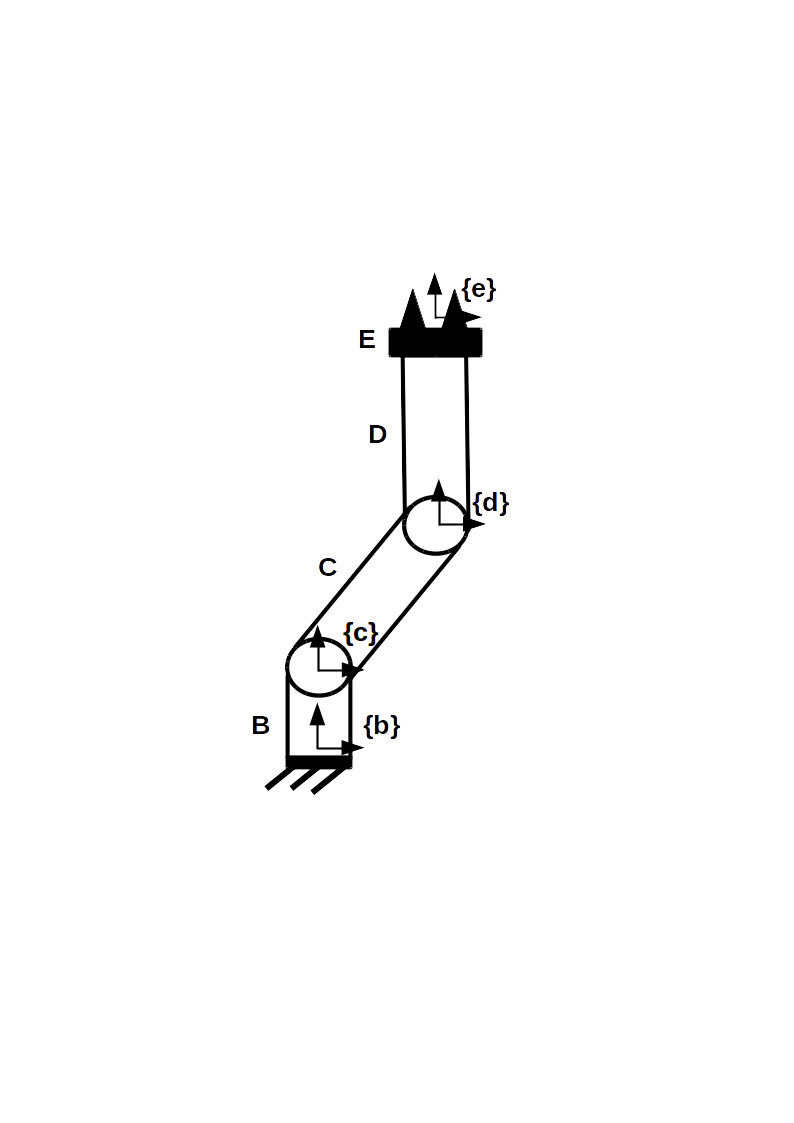
\includegraphics[width=100mm, trim=0 250 0 200]{pictures/semantics_usecases}
\caption{3-link manipulator in order explain all the four use cases}
\label{fig:semanticsusecases}
\end{figure}

The relative pose of the rigid body B w.r.t. the body A can be given as $Pose ((c,{c}) | C, (b,{b}) | B)$ where (c, \{c\}) represents the position and orientation of the body C w.r.t. the reference body B. The first use case for the inverse and compose operations can be computed as follows
\begin{align}
& ^{\{b\}|B}T_{\{c\}|C} = ^{\{c\}|C}T^{-1}_{\{b\}|B} \\
& ^{\{b\}|B}T_{\{d\}|D} = ^{\{b\}|B}T_{\{c\}|C} \cdot ^{\{c\}|C}T_{\{d\}|D} \\
& ^{\{b\}|B}T_{\{e\}|E} = ^{\{b\}|B}T_{\{d\}|D} \cdot ^{\{d\}|D}T_{\{e\}|E}
\end{align}

The second use case involves the semantics checking
\begin{align}
& Pose(\{c\}|C, \{b\}|B) = inverse(Pose(\{b\}|B, \{c\}|C)) \\
& Pose(\{d\}|D, \{b\}|B) = compose(Pose(\{d\}|D, \{c\}|C), Pose(\{c\}|C, \{b\}|B)) \\
& Pose(\{e\}|E, \{b\}|B) = compose(Pose(\{e\}|E, \{d\}|D), Pose(\{d\}|D, \{b\}|B))
\end{align}

The third use case involves the coordinates semantic checking which also considers the coordinate frame check as given below
\begin{align}
& PoseCoord(\{c\}|C, \{b\}|B, [b]) = inverse2(PC(\{b\}|B, \{c\}|C, [c])) \\
& PoseCoord(\{d\}|D, \{b\}|B, [b]) = compose(PC(\{d\}|D, \{c\}|C, [c]), PC(\{c\}|C, \{b\}|B, [b])) \\
& PoseCoord(\{e\}|E, \{b\}|B, [b]) = compose(PC(\{e\}|E, \{d\}|D, [d]), PC(\{d\}|D, \{b\}|B, [b]))
\end{align}

where PC is the pose coordinates. The $PoseCoord(\{d\}|D, \{b\}|B, [b]$ is determined by composing the pose coordinates $PC(\{c\}|C, \{b\}|B, [b])$ and the pose coordinates \\$PC(\{d\}|D, \{c\}|C, [c])$ as given in the above equation. The reference point, reference orientation frame, and the reference body of the first pose in the compose operation in equation 3.11 have to be equal to the point, orientation frame, and the body of the second pose. The fourth use case checks the coordinate semantics of the poses that results from the inverse, compose operations can be verified from the arguments of the compose operation. At last the numerical operations based on the coordinate representations can be generated from the semantic equations of the third use case. If the software is built based on these semantic rules, it is possible to avoid the logical errors in the geometrical relation semantics between the rigid bodies. The possible logical error in the pose related semantics is that the poses and the orientation coordinate representations are composed in the wrong order. Since the coordinate system selection varies from one developer to another as depicted in Fig.~\ref{fig:diffinconventions} and the order of the composition indicates the geometric relation between the rigid bodies which is not commutative.

\subsubsection*{Motion and force related semantics}

The motion transforms discuss about the semantics that needs to be considered to transmit the velocity or the acceleration of a particular rigid-body to its successor body. The motion transforms are considered as easy to implement but the real problem comes when different libraries are combined together for the purpose of achieving the common goal which in-turn introduces the different semantic representations used by the different authors i.e., Orocos KDL~\cite{smits2011kdl}, Simbody~\cite{sherman2011simbody}, Atkeson et. al.~\cite{Atkeson}, Featherstone~\cite{featherstone2014rigid}. It is only fair to explain the concept of kinematics before getting into further details. Kinematics is the study of motion of the objects without taking the forces into consideration that cause the motion. The kinematics can be classified into forward and inverse kinematics. This work uses only the forward kinematics which includes position, velocity and acceleration kinematics. The forward kinematics have undergone logical changes comparing the previous RnD~\cite{RnD2Rajagopal} since the implicit conventions are analyzed and briefed in a detailed way. The twist or acceleration of a body has the point, reference and target body, coordinate frame information attached to it in the level of semantics. 

\subsection{Orocos KDL's geometrical relation semantics}

It is really important to understand the semantics used by the library before jumping into the implementation details of it. If the developer fails to do so, the computations are going to be introduced with the logical errors in different levels such as the pose, motion and force level. So, lets start with the semantics considered by the Orocos KDL~\cite{smits2011kdl} library and then the changes required to keep up with the standard semantic conventions. 

\subsubsection*{Semantics with poses}

The position and orientation of the segment in KDL can be given as

\begin{equation}
\begin{aligned}
& p : Position (tip_i, joint_i) \\
& R : Rotation ([tip_i], [root_i])
\end{aligned}
\end{equation}

where p represents the position of the $tip_i$ w.r.t. the $joint_i$ position and R represents the relative orientation of the frame $[tip_i]$ w.r.t. the frame $[root_i]$.

\subsubsection*{Semantics with forward velocity kinematics}

A twist is the combination of both the translational and angular/rotational velocities. The twist $v_i$ of the $body_i$ can be computed by adding the twist of the predecessor body with the twist contribution of the $joint_i$~\eqref{eq:velocitymotiontransform}.

\begin{equation}
v_i = \overbrace{^iX_{i-1}\cdot v_{i-1}}^{transform} \overbrace{+}^{compose}  \overbrace{S_i\cdot \dot{q}_i}^{V_J}
\label{eq:velocitymotiontransform}
\end{equation}

where the twist at joint i is projected into the joint's internal axis using the subspace matrix $S_i$, the motion transform transmits the twist contribution of the predecessor body $v_{i-1}$ to the current body $v_i$. The addition operation of the twists in the equation~\eqref{eq:velocitymotiontransform} can be viewed in two different ways. At first, it can be seen that the numerical calculation adds the twists of two different bodies with the simple matrix operations. Another consideration is that the addition of the twists has to be semantically right. The compose operation adds the Twist($S_i\cdot \dot{q}_i$) with the Twist($^iX_{i-1}\cdot v_{i-1}$) to get the Twist $v_i$. Based on the coordinate semantic representation of the twist during the integration discussed by~\cite{geometicsemanticspart1}~\cite{geometicsemanticspart2}, the twists can be integrated only when the twists are represented at a common point and at the same coordinate frame. If the semantics of the twists are different from these conventions then the developer has to consider the change point operation and change coordinate operation to form the proper geometrical relation between the rigid bodies.

\begin{figure}[h]
\centering
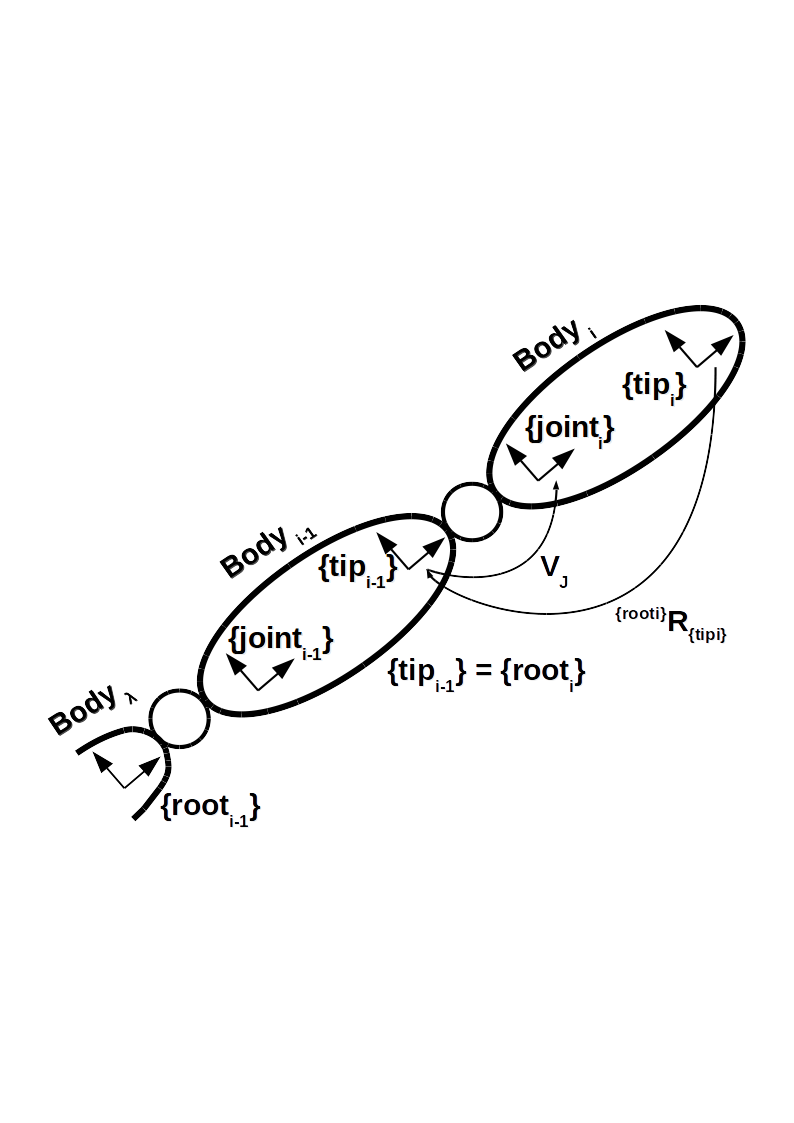
\includegraphics[width=100mm, trim=0 250 0 250]{pictures/kdl_rigidbody_semantics}
\caption{Velocity motion transform semantics used in Orocos KDL}
\end{figure}

The twist of the $body_i$ w.r.t. the $Body_{i-1}$ at point $joint_i$ can be given as

\begin{equation}
v_J = Twist(joint_i|Body_i, Body_{i-1}, [root_i])
\label{eq:twistofthecurrentbody}
\end{equation}

where $v_J$ represents the semantics representation of the twist at joint i. The twist of the previous body can be given semantically 

\begin{equation}
v_{i-1} = Twist(joint_{i-1}|Body_{i-1}, Body_w, [root_{i-1}])
\label{eq:twistofthepreviousbody}
\end{equation}

where $Body_w$ is the predecessor of the $Body_{i-1}$ or it can be considered as the ground body. The forward velocity kinematics are supposed to integrate the twists of the current body $V_J$ as given in the equation~\eqref{eq:twistofthecurrentbody} and the twist of the predecessor $v_{i-1}$. Where the semantics checking fails due to the reason that both twists are represented in the different coordinates and in different point. So, the change point and the change of coordinates are really important for the compose operation and it is computed in the following equations. The change point operation can be semantically given as
\begin{equation}
\begin{aligned}
v'_{i-1} = {} & Twist(joint_{i-1}|Body_{i-1}, Body_w,  [root_{i-1}]) \\ 
& .changePoint(joint_i|Body_{i-1}, joint_{i-1}|Body_{i-1}, [root_{i-1}])
\end{aligned}
\end{equation}

The change point operation in the predecessors' velocity result in the following semantics

\begin{equation}
v_{cp} = Twist(joint_i | Body_{i-1}, Body_w [root_{i-1}])
\end{equation}

where $v_{cp}$ represents the change point operation on the twist and the change coordinate operation on the same can be semantically extracted as
\begin{equation}
\begin{aligned}
v_{cc} = {} & TwistCoordinates(joint_i|Body_{i-1}, Body_w, [root_i]) \\ & .changeCoordinateFrame(OrientationCoordinates([root_{i-1}]|Body_w, \\&[root_i]|Body_w, [root_i]))
\end{aligned}
\end{equation}

The change coordinate frame $v_{cc}$ results with the following semantics 

\begin{equation}
v_{cc} = Twist(joint_i | Body_{i-1}, Body_w, [root_i])
\label{eq:predecessorstwistwithsemanticchanges}
\end{equation}

Now, the twists in the equations~\eqref{eq:predecessorstwistwithsemanticchanges} and~\eqref{eq:twistofthecurrentbody} are semantically correct for the compose operation.

\begin{equation}
v_i = compose(v_J, v_{cc})
\end{equation}

and the geometric relation of the twist $v_i$ results in the following equation
\begin{equation}
v_i = Twist(joint_i | Body_i, Body_w, [root_i])
\end{equation}

\subsubsection*{Semantics with forward acceleration kinematics}

Similar to the velocity motion transform, the acceleration semantics can be extracted for the KDL library. The acceleration kinematics can be computed by

\begin{equation}
a_i = \overbrace{^iX_{i-1}\cdot a_{i-1}}^{transform} \overbrace{+}^{compose} \overbrace{S_i\cdot \ddot{q}_i}^{a_J} \overbrace{+}^{superpose}  \overbrace{v_i \times S_i\cdot \dot{q}_i}^{Bias}
\label{eq:accelerationkinematicsandsemantics}
\end{equation}

where the first compose operation of the acceleration at the joint i with the predecessor body i-1 can be done as same the velocity kinematics which involves motion transmission. The second addition operator is referred as superpose operation since the physical meaning of the addends are different. The above equation~\ref{eq:accelerationkinematicsandsemantics} can be simply viewed as the following 

\begin{equation}
a_i = a_{i-1} + a_J + bias
\label{eq:simplifiedacceleration}
\end{equation}

The acceleration at joint i has the following relation

\begin{equation}
a_J = Acceleration(joint_i | Body_i, Body_{i-1}, [root_i])
\end{equation}

The acceleration of the body i-1 can be represented with the geometric relations as

\begin{equation}
a_{i-1} = Acceleration(joint_{i-1} | Body_{i-1}, [root_{i-1}])
\end{equation}

The change point and coordinates of the predecessor body's acceleration. The change point operation can be computed as
\begin{equation}
\begin{aligned}
a_{cp} = {} & Acceleration(joint_{i-1}|Body_{i-1}, Body_w,  [root_{i-1}]) \\ 
& .changePoint(joint_i|Body_{i-1}, joint_{i-1}|Body_{i-1}, [root_{i-1}])
\end{aligned}
\end{equation}

which results in the following equation
\begin{equation}
a_{cp} = Acceleration(joint_i, Body_{i-1}, Body_w, [root_{i-1}])
\end{equation}

The change coordinate frame can be done with the following equation

\begin{equation}
\begin{aligned}
a_{cc} = {} & AccelerationCoordinates(joint_i|Body_{i-1}, Body_w, [root_i]) \\ & .changeCoordinateFrame(OrientationCoordinates([root_{i-1}]|Body_w, \\&[root_i]|Body_w, [root_i]))
\end{aligned}
\end{equation}

which results in the following equation
\begin{equation}
a_{cc} = Acceleration(joint_i, Body_{i-1}, Body_w, [root_i]) 
\end{equation}

Now the semantics checking is succeeded and the superpose operation is performed $(a_{cc} + a'_i)$ based on~\cite{traversaro2016multibody} in equation~\ref{eq:simplifiedacceleration} results in the following geometric relation semantics

\begin{equation}
a_i = Acceleration(joint_i | Body_i, Body_w, [root_i])
\label{eq:finalacceleration}
\end{equation}

\subsubsection*{Semantics with forces and torques}

The recursive Newton-Euler formulation~\cite{smits2011kdl} in the spatial form which is used by the KDL library can be given as

\begin{equation}
f_I = I_i\cdot a_i + v_i\cdot \times (I_i\cdot v_i) - f_{{ext}_i}
\end{equation}

where the acceleration $a_i$ is mapped with the function I which gives the forces required, I represents the inertia of the rigid-body i. The semantics of the inertia has the information such as frame, and the body. The reference frame of the inertia can be assumed to be the frame that is  attached in the target body as inertia represents the particular body. So the semantics of the operation $I_i\cdot a_i$ is same as the semantics of $a_i$ given in the equation~\eqref{eq:finalacceleration}. The other forces such as bias and external forces should have the same semantics as the first term for the integration operation. The torques can be extracted by projecting the spatial forces into the joint's internal axis as 

\begin{equation}
\tau_i = S_i\cdot f_i
\end{equation}

where S represents the subspace matrix that projects the force into internal axis of the joint. It is assumed that the torque is represented in the target joint frame as the joint has a reference as well as the target frame. The reference frame is present in the predecessor and the target frame is the one which is attached in the target body that is being referred to. Formally, the force transform does the change point and coordinate frame operations as same as the semantics derived in the velocity and acceleration kinematics and once the semantics with the transform matches up with the semantics of $f_i$, the compose operation can be performed.

\subsection{Featherstone's geometrical relation semantics}

Before getting into the details of the pose, motion and force semantics, it is mandatory to go through the conventions used for the rigid body.

\begin{figure}[h]
\centering
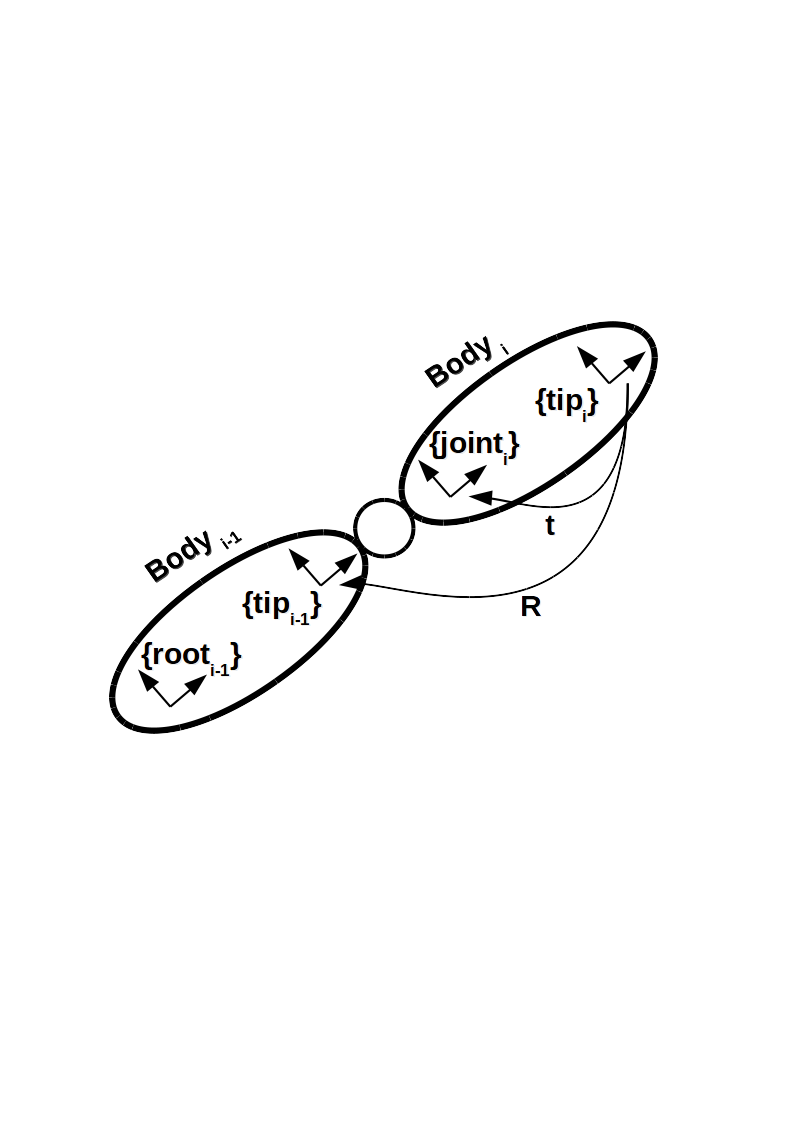
\includegraphics[width=100mm, trim=0 250 0 250]{pictures/featherstone_rigidbodyi}
\caption{Rigid body semantics in the article~\cite{featherstone2014rigid}}
\end{figure}

\subsubsection*{Semantics with poses}
The position and orientation of the segment is the same as the KDL segment 

\begin{equation}
\begin{aligned}
& p : Position (tip_i, joint_i) \\
& R : Rotation ([tip_i], [root_i])
\end{aligned}
\end{equation}

\subsubsection*{Semantics with forward velocity kinematics}

In~\cite{featherstone2014rigid}, author considers the point at which the twist is represented is same as the origin of $root_i$ hence there is absolutely no need of either the change point and orientation coordinates. The change point and orientation coordinates are accounted in the form of spatial transforms. This method is the inverse of the semantic representations used by KDL.

\begin{equation}
v_J = Twist(root_i|Body_i, Body_{i-1}, [root_i])
\end{equation}

\subsubsection*{Semantics with forward acceleration kinematics}

The acceleration semantics can be given as

\begin{equation}
a_J = Twist(root_i|Body_i, Body_{i-1}, [root_i])
\end{equation}

\subsubsection*{Semantics with forces and torques}
The semantics for forces, torques and force transforms in this rigid body algorithm can be extracted as same as the KDL. The only difference is that the propagation of forces between the rigid bodies does not require the change point and coordinate frame operation. 

\section{Inertial parameter estimation}

The random trajectories were used for the identification procedure in the previous work~\cite{RnD2Rajagopal}. These trajectories are not periodic and it is not possible to make sure whether the whole robot workspace is covered or not. With excitation trajectory analysis concentrating on even the smallest changes of the dynamic model parameters, we can better estimate the parameters.

\subsection{Excitation trajectories}
This section discusses the method that produces optimal robot excitation trajectories that are suitable for identifying the dynamic model parameters with trajectories covering the most of the workspace~\cite{SweversJ1997Orea}~\cite{vantilt2015optimal}. The parameterization and optimization of the robot excitation trajectories can be generated with the following method. 

\subsubsection*{Parameterization of the excitation trajectories}

This section is based on an understanding from~\cite{SweversJ1997Orea}~\cite{swevers}.
The aim of the trajectory parameterization method is to generate the periodic and bandlimited data that improves the accuracy in parameter estimation. The parameterization can be done by using the finite Fourier series which is the sum of harmonic sine and cosine functions. This function generates the data for all the manipulator joints $N$ and it can be generated using the following equation

\begin{equation}
q_i(t) = \sum_{j=1}^{N_i} \frac{a{_j^i}}{w_f\cdot j} sin(w_f\cdot j\cdot t) - \frac{b{_j^i}}{w_f\cdot j} cos(w_f\cdot j\cdot t) + q_i(0)
\label{eq:ffs}
\end{equation}

where $w_f$ represents the frequency which is common for all the joints, t represents time, $a{_j^i} b{_j^i}$ represents the coefficients or amplitude of the functions sine and cosine, $q_i(0)$ is the initial position of the joint. The Fourier series has the periodic function with the period $T_f = 2\pi/w_f$ and it has 2N + 1 parameters that represent the DoF for the trajectory optimization. The basic idea of the parameterization of the trajectory involves selecting a low fundamental frequency which offers the longer excitation period. The velocities and accelerations can be generated by taking the derivative and double derivative of the equation~\eqref{eq:ffs}.

\subsubsection*{Optimization of the excitation trajectories}

The optimal values of the coefficients can be selected through experiments based on the trial-and-error method or by solving the non linear optimization problem with the constraints imposed on the robot motion~\cite{swevers}. The d-optimality criterion is used as an objective function that depends on the robot trajectory data that has been applied to the observation matrix K and the resulting matrix is stacked up vertically with the feasible solutions. The general optimization problem~\cite{boyd2004convex} finds the best possible solution from the available solutions. The main objective of the optimization problem is to minimize the objective function f(x) with the input vector x is subject to the equality and inequality constraints. In this work, x has parameters a, b, q(0) to optimize/minimize and the f(x) can be optimized with two different methods as given below. The determinant of the matrix gives sufficient details about the scores of the optimization. 
\begin{equation}
f(x) : min(a{_j^i}, b{_j^i}, q_i(0)) det(K^T\cdot K)
\end{equation}

\begin{flushleft}
If the $det(K^T\cdot K)$ is equal to 0, it means that the matrix $K^TK$ is singular and the rows and columns of the matrix $K^TK$ are linearly not independent. Whereas the other method is based on finding the condition number
\end{flushleft}

\begin{equation}
f(x) : min(a{_j^i}, b{_j^i}, q_i(0)) cond(K^T\cdot K)
\end{equation}

The above given equation is constructed based on the approach given by~\cite{vantilt2015optimal}\cite{swevers}. The large condition number means that the small change in the observation matrix can lead to a large change in output hence the highest scores are considered to be inefficient. The equality constraints of this optimization problem can be given as
\begin{align*}
& h^1(x) : lower\_joint\_limit <= q(a, b, q_0) <= upper\_joint\_limit \\
& h^2(x) : lower\_joint\_limit <= \dot{q}(a, b, q_0) <= upper\_joint\_limit \\
& h^3(x) : lower\_joint\_limit <= \ddot{q}(a, b, q_0) <= upper\_joint\_limit \\
& h^4(x) : lower <= FPK(q) (no collision)
\end{align*}

The K matrix is constructed by vertically stacking up the result of the way-points of the optimized trajectory that is applied to the K matrix. 
\begin{equation}
K = \begin{vmatrix}
K(q(1), \dot{q}(1), \ddot{q}(1)) \\
.\\
.\\
.\\
K(q(N), \dot{q}(N), \ddot{q}(N)) \\
\end{vmatrix}
\end{equation}

\newpage

\section{Model-based controller for a non-linear system}

This section explains the model-based controller for the non-linear system which is considered in this work. As discussed in the previous sections, the joint-space controller is implemented in this work and the pictorial representation is shown in Fig.~\ref{fig:jointspacecontroller}.

\begin{figure}[h]
\centering
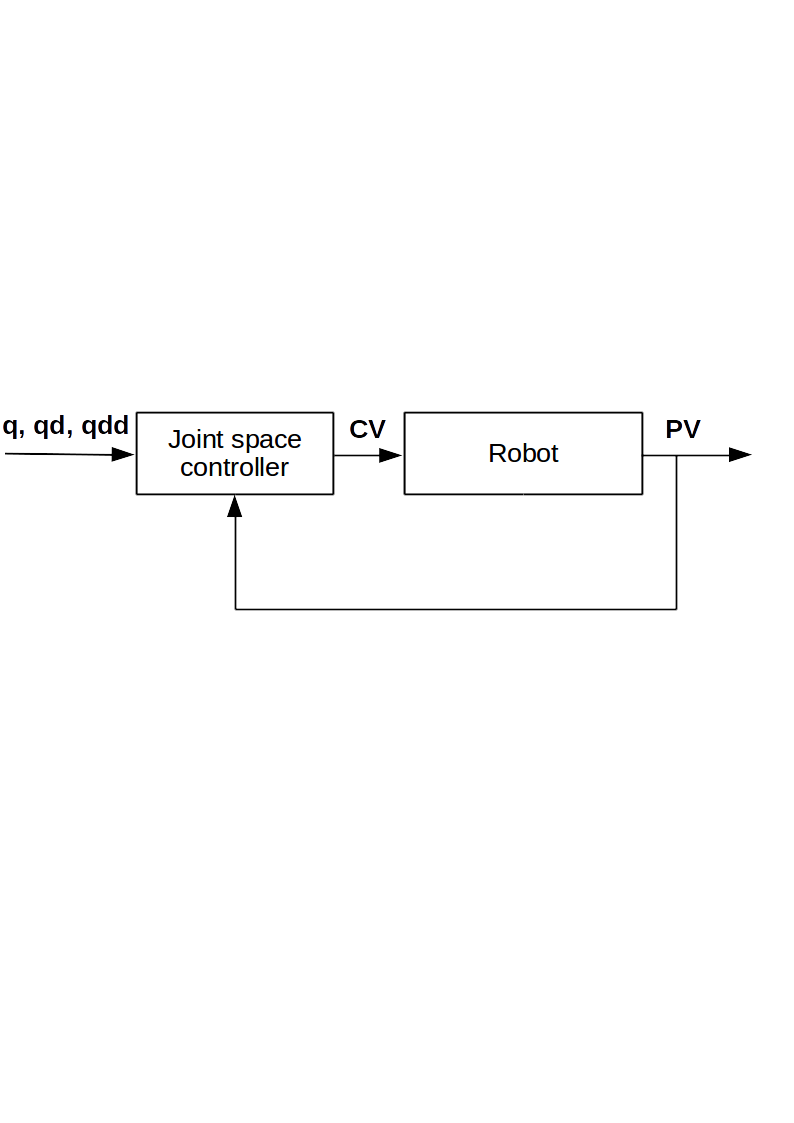
\includegraphics[width=100mm, trim=0 400 0 300]{pictures/jointspacecontroller}
\caption{Joint space controller}
\label{fig:jointspacecontroller}
\end{figure}

This work uses the advanced joint control mode that commands torque to the manipulator joints in order to achieve the particular target. Since the controller is attached in the joint space of the youBot manipulator and it is not defined in the operational task space. The accuracy of this control method heavily relies on the accuracy of the dynamic model parameters and the encoder that is attached to the individual joints of the manipulator. The following Fig.~\ref{fig:simpletorquemode} gives overview of operations before commanding the torque to the real system.

\begin{figure}[h]
\centering
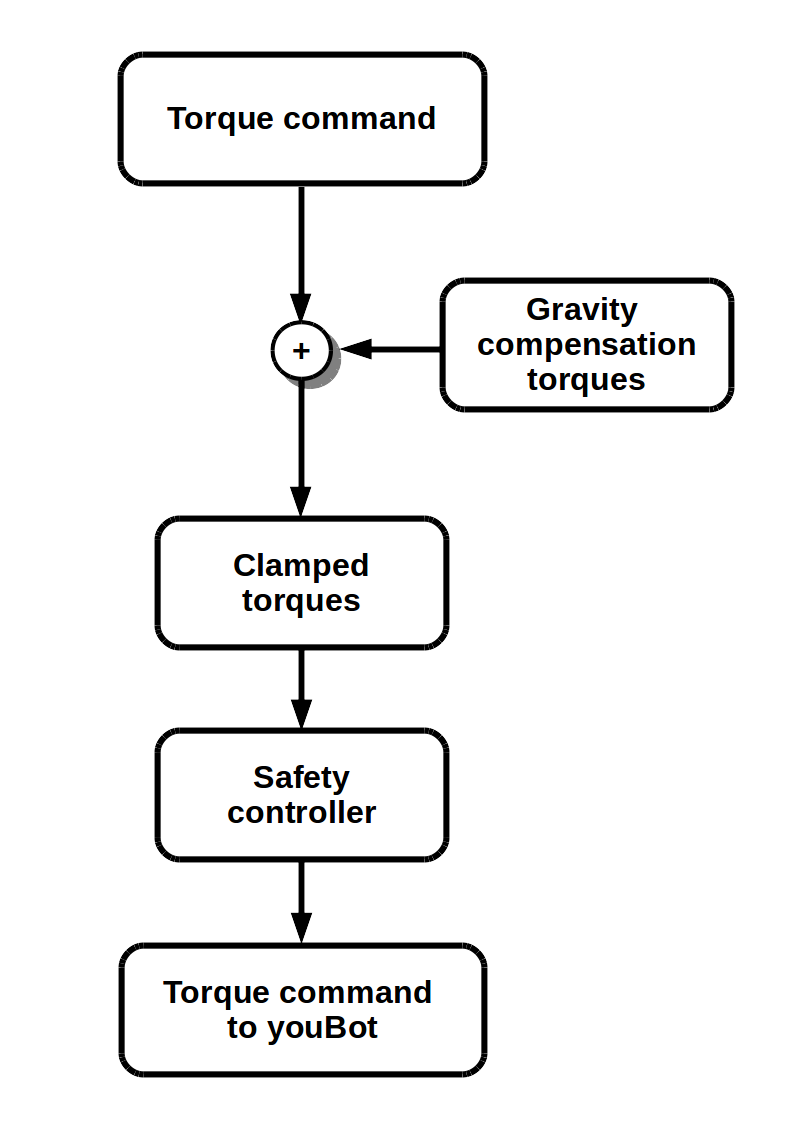
\includegraphics[width=60mm, trim=0 20 0 20]{pictures/torque_mode}
\caption{Torque control mode}
\label{fig:simpletorquemode}
\end{figure}

In addition to the commanded torque, the gravity compensation torque is also added as a feed-forward mechanism. The result of this addition goes through clamping and this feature is particularly important in handling the out-of-bounds or NaN torque commands. The class diagram for the package implemented in this work is depicted in Fig.~\ref{fig:classdiagram}.

\begin{figure}[h]
\centering
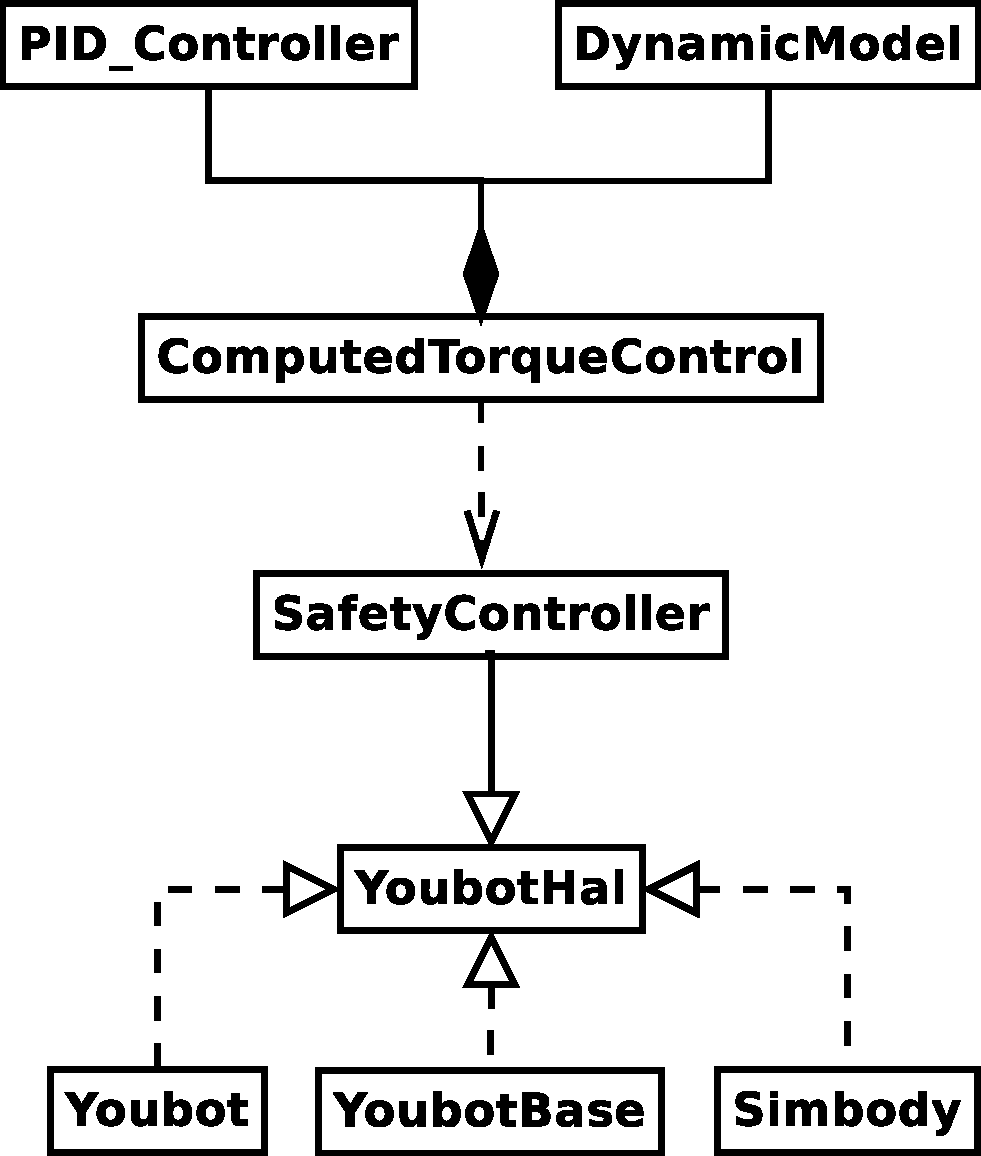
\includegraphics[width=50mm]{pictures/classdiagram_package.pdf}
\caption{The complete class diagram for the model-based controller which is implemented in this work.}
\label{fig:classdiagram}
\end{figure}

\subsection{Dynamic model based on Orocos KDL}

There are two kinds of controllers as depicted in Fig.~\ref{fig:basicapproach} and~\ref{fig:alternateapproach}. The approach specified in Fig.~\ref{fig:basicapproach} is implemented on the youBot manipulator where the problem persists with the inaccurate rotational inertia parameters, hence the alternate method is chosen as depicted in Fig.~\ref{fig:alternateapproach}. An important feature of consideration in computed-torque control~\cite{muggler2013torque} is the dynamics of the manipulator whereas the joint position or velocity control do not account the dynamics and the joint configuration. Dynamics is the field of study where the relationship between the forces and the motion are investigated. The general equation of motion can be written as based on~\cite{muggler2013torque}

\begin{equation}
\tau = M(q)\ddot{q} + C(q, \dot{q})\dot{q} + G(q, \dot{q})
\label{eq:dynamicmodel}
\end{equation}

where $\tau$ is the torque applied to the manipulator links. M represents the manipulator inertia matrix which comprises of mass, moments of inertia and C represents the Coriolis and Centrifugal forces which basically depends on the joint position and velocity. G represents the vector of external forces acting on the manipulator links such as gravity and friction effect. The non-linear dynamic equation of motion for the manipulator can be used to compute the joint torques for the given joint position, velocity and acceleration. The dynamics equation~\eqref{eq:dynamicmodel} has non-linear functions M, C and G of the model parameters. In order to control the non-linear system with the linear control, it is important to select the control input $\tau$ that follows the desired trajectory. The above equation~\eqref{eq:dynamicmodel} can be rewritten as 

\begin{equation}
\ddot{q} = M^{-1}(q) (\tau - C(q, \dot{q})\dot{q} - G(q, \dot{q}))
\label{eq:forwarddynamics}
\end{equation}

if the non-linear terms in the above equation~\eqref{eq:forwarddynamics} are cancelled, it is possible to apply the linear control strategies. If the non-linear terms are known, it is possible to choose the control input as given in the equation~\eqref{eq:knownnonlinearterms}for the PD control loop 

\begin{equation}
\tau = M(\theta) \ddot{q} + C(\theta, \dot{\theta})\dot{\theta} + G(\theta, \dot{\theta})
\label{eq:knownnonlinearterms}
\end{equation}

The following equation can be regarded as the closed-loop error dynamics where the $K_D$ term is equal to 0 and it is referred from the article~\cite{Chung2016}

\begin{equation}
\dot{q}_d = (q_e\cdot K_p + \sum q_e\cdot K_i)
\end{equation}

\begin{equation}
\ddot{q} = limit(\dot{q}_e\cdot K_p + \sum \dot{q}_e\cdot K_i)
\end{equation}

where $K_p, K_i$ represents the proportional and derivative gains of the PI control respectively and the gains are going to be optimized by manually tuning for each and every link of the manipulator. The manual tuning can be done based on the experiments by investigating the individual step responses for the particular joints. Otherwise, overshoot occurs when the gains are not optimal and the stability of the system can’t be achieved. $q_e, \dot{q}_e$ represents the position and the velocity error as given in the following equations

\begin{equation}
q_e = q_d - q_m
\end{equation}
\begin{equation}
\dot{q}_e = \dot{q}_d - \dot{q}_m
\end{equation}

where $q_d$ represents the desired joint angle and $q_m$ represents the measured joint angle of an individual joint. $\dot{q}_d$ represents the desired joint velocity and $\dot{q}_m$ is the measured joint velocity of an individual joint.

Alternate method is chosen in this work which is a simple computed-torque control scheme. The dynamic model gets the measured joint positions and velocities from the manipulator joints with the zero acceleration. The $\ddot{q}$ is zero as depicted in Fig.~\ref{fig:alternateapproach}, so the equation~\eqref{eq:dynamicmodel} can be rewritten as 

\begin{equation}
\tau = C(q_m, \dot{q_m})\cdot \dot{q_m} + \tau_g(q_m)
\end{equation}

The above equation can't accelerate the joints but it computes the gravitational term and the Coriolis, Centrifugal terms. 

\subsubsection*{Gravity compensation}

The gravity compensation torques $\tau_g(q)$ are computed based on the KDL model which has been specified in the previous section. The model based gravity compensation on the manipulator joints and the gravity compensation for joint 1 and 5 can not be computed since these two joints are fixed.

\subsubsection*{Friction modelling and compensation}

Friction is one of the important effects that need to be accounted in the control systems. The control systems try to compensate the friction effects by tuning the controller gains to a higher value, so there is a need of a friction model and the compensation technique. Friction has a significant effect on the mechanical systems where the precision is the ultimate goal and there are many friction modelling schemes have been introduced~\cite{corberan2012haptic}. It can be classified into static and kinetic(dynamic) friction.

\SetKw{KwBy}{by}

\begin{algorithm}
    \SetKwInOut{Input}{Input}
    \SetKwInOut{Output}{Output}

    \underline{directionOfDesiredVelocity} $(\dot{q}_d)$\;
    \Input{$\dot{q}_d$}
    \Output{$scale$}
    \uIf{$(\dot{q}_d < 0$}
    {
    		scale = -1;
		return scale;
    }
    \uElseIf{$\dot{q}_d > 0$}
    {
    		scale = 1:
    		return scale;
    }
    \uElse
    {
    		scale = 0;
    		return scale;
    }
    \caption{Direction of the desired velocity}
\end{algorithm}

\begin{algorithm}
    \SetKwInOut{Input}{Input}
    \SetKwInOut{Output}{Output}

    \underline{frictionModel} $(\dot{q}_d, \dot{q}_m)$\;
    \Input{$m, \dot{q}_m,$,\\ $n\gets5$,\\$static\_friction$,\\$kinetic\_friction$}
    \Output{$\tau_f$}
    \uIf{$|\dot{q}_d| > 0.0$}
    {
    \For{$joint\_number\gets0$ \KwTo $n$ \KwBy $1$}{
      \uIf(\tcc*[h]{The joint is not moving}){$|\dot{q}_m| <= 0.01$}
      {
        $\tau_s = static\_friction[joint\_number] \cdot sgn(\dot{q}_d[joint\_number])$\;
      	$\tau_f$ = $\tau_s$\;
      }
      {
        \tcc{Coulomb friction modelling}
      	%$\tau_c = \mu\cdot \tau_N \cdot sgn(\dot{q}_d)$\;
      	$\tau_k = \tau_c\cdot sgn(\dot{q}_d[joint\_number])$\;
		\tcc{Kinetic friction torque}
        $\tau_f$ = $\tau_k$\;
      }
    }
    }

    return $\tau_f$\;
    \caption{Friction observer}
\end{algorithm}

The friction values are identified based on trial-and-error method and the static friction estimates are readily available~\cite{RnD2Rajagopal}. The Coulomb friction is used to model the kinetic friction where the torque is constant irrespective of the input velocity value as given in the Fig.~\ref{fig:frictionmodel}. The Coulomb friction basically restricts the rotational motion of the joint. The static friction torque is applied to a particular joint makes the joint to overcome the static friction and it starts to move. This particular technique is referred to static friction compensation. Once the joint is in motion, the kinetic or dynamic friction torque is applied as the compensation term. This technique is referred to kinetic friction compensation.

\begin{figure}[h]
\centering
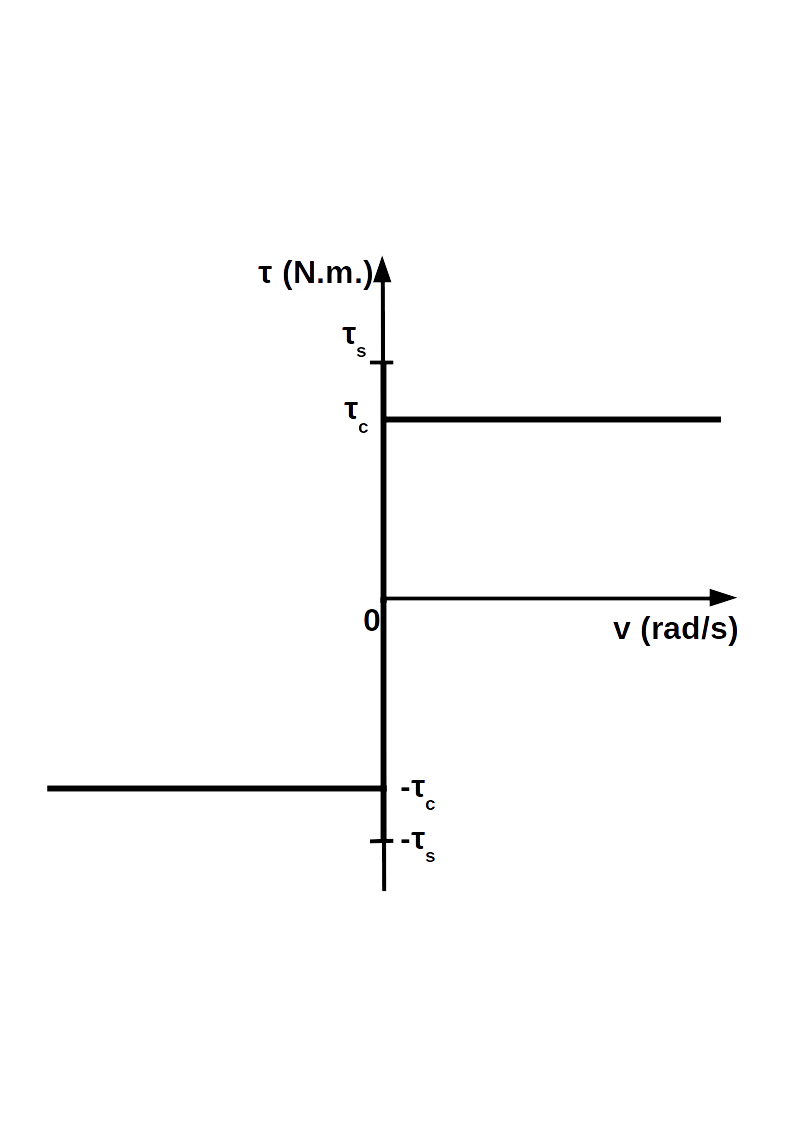
\includegraphics[width=80mm, trim=0 180 0 220]{pictures/friction_staticandcoulomb}
\caption{Friction model}
\label{fig:frictionmodel}
\end{figure}

\newpage
\subsection{Computed-torque control}

Computed-torque control technique is widely used in the industrial robots and it works with the feedback mechanism to control the non-linear systems. The class diagram for the computed-torque controller is shown in Fig.~\ref{fig:classdiagram_computedtorquecontrol}. It is possible to apply the linear control strategies i.e., PI controller after the system is linearized. The linearization is achieved with the help of the KDL based ID solver which is the recursive Newton-Euler formulation. The working principle of the cascade controller is explained in the following section.

\begin{figure}[h]
\centering
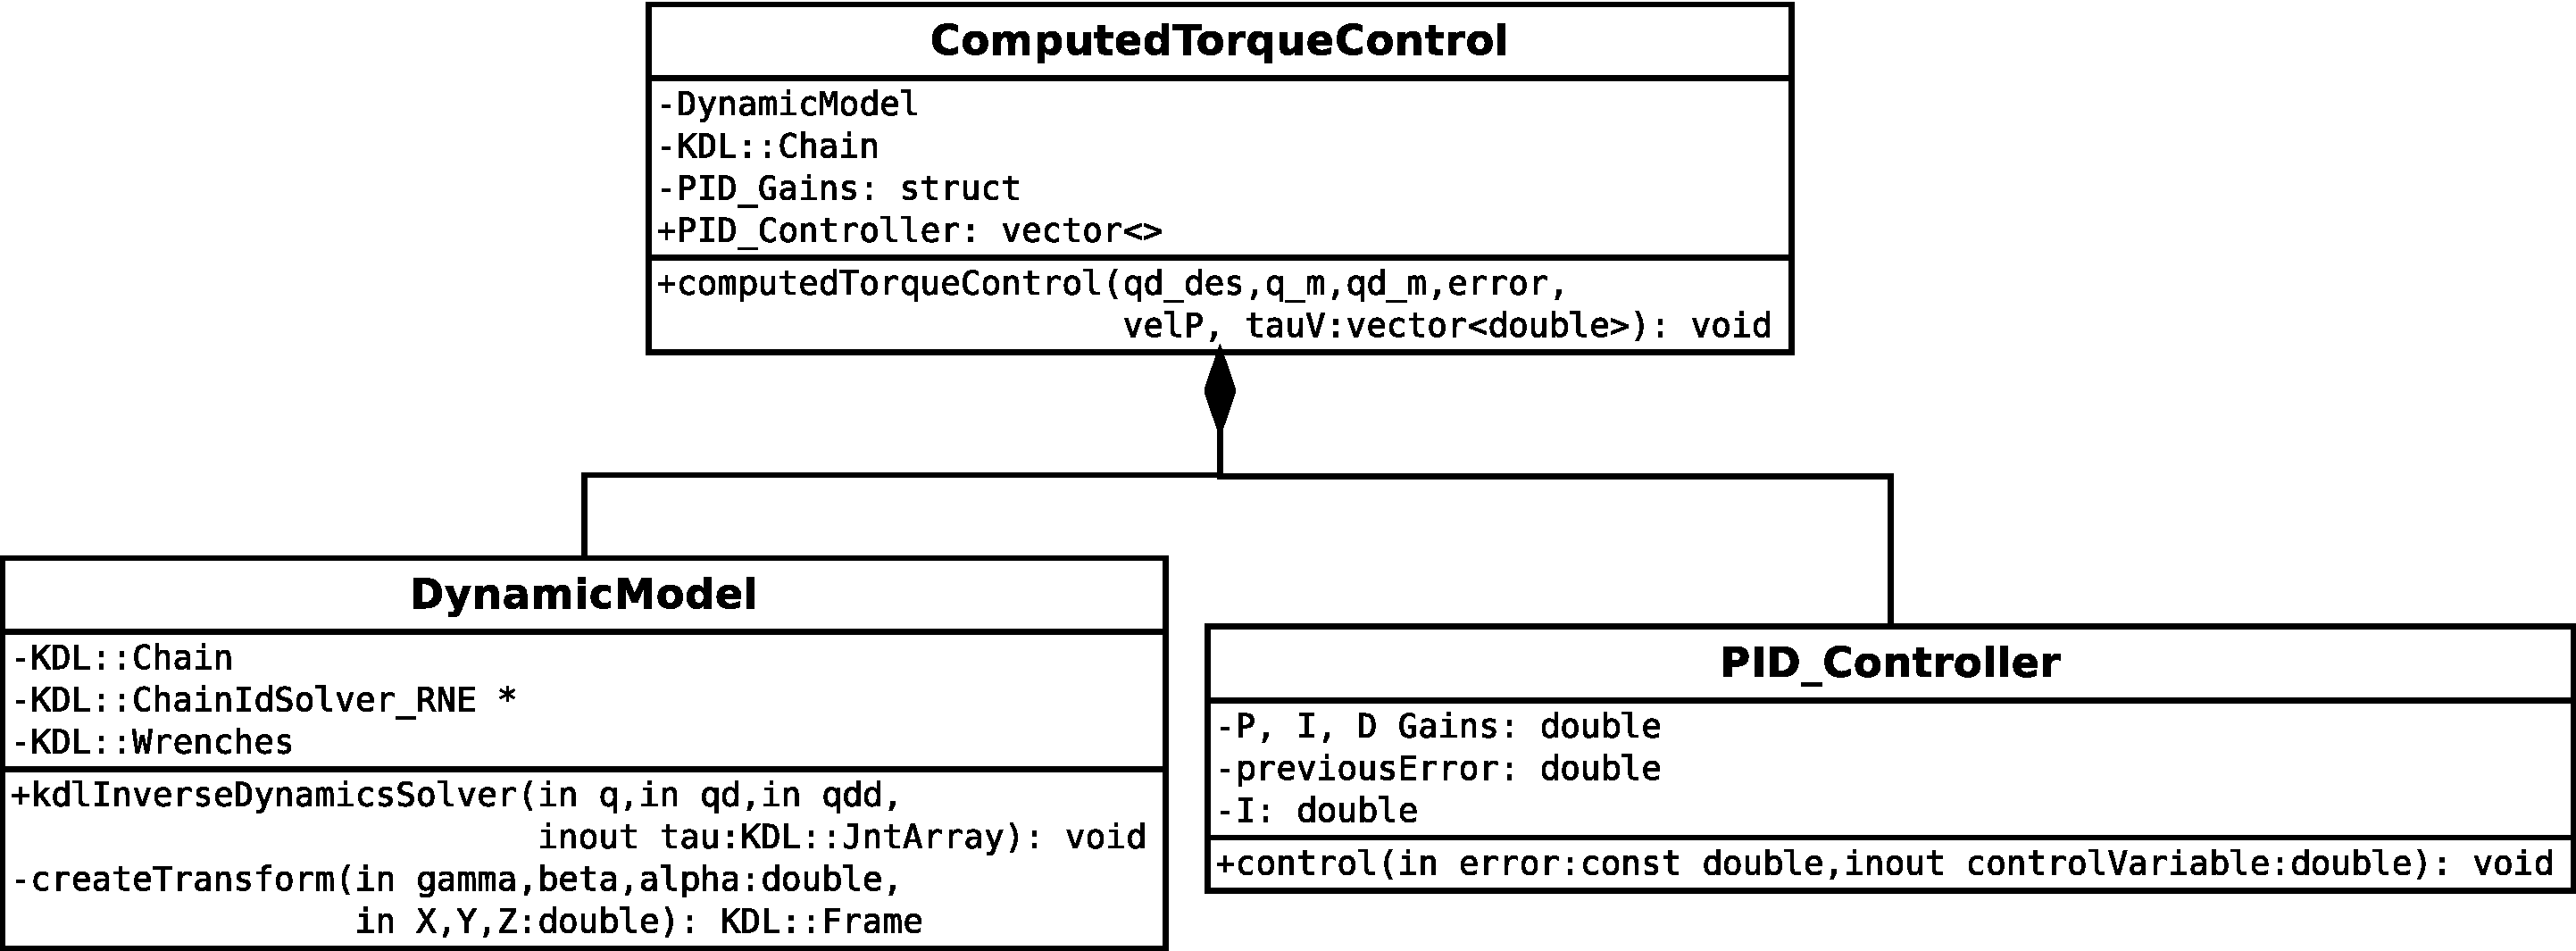
\includegraphics[width=150mm]{pictures/class_diagram_computedtorquecontrol.pdf}
\caption{The class diagram for the computed-torque control.}
\label{fig:classdiagram_computedtorquecontrol}
\end{figure}

\subsubsection*{Cascade PI controller}

Most of the control applications use only the single-loop control for solving a control problem. The basic definitions of this section are referred from~\cite{cascadedcontrol}~\cite{astrom1995pid}. But this work uses the cascade control method that has two controllers where one controller's output drives the set-point of the secondary controller. The cascade control system can have one or more inner loops inside the main control loop (outer-loop), and the controllers are in cascade. The advantages of the cascade controller is the fast response and the better disturbance rejection. This work is not considering the D-term of the controller as it is assumed that the damping factor is already present in the system as the friction force. The main loop can be called as master loop and the inner loop is the secondary controller. The position PI controller is attached in the outer loop and the velocity PI controller is attached in the inner-loop. The position PI controller output is limited to a desired velocity before feeding it into the velocity controller. Based on this limiting feature, the velocity of the joint can be controlled and saturated when the limits are breached. It is particularly useful in avoiding the high-speed motions in joint level. The presence of the dynamic model makes this controller model-driven whereas the system is considered to be pure cascade PI control scheme if the dynamic model is not considered. 

\begin{center}
\begin{tikzpicture}[auto, node distance=2cm,>=latex']
    \node [input, name=input] {};
    \node [block, right of=input, node distance=2.5cm] (pcontrol) {\textbf{\shortstack{Position\\ controller}}};
    \node [block, right of=pcontrol, node distance=3cm](vcontrol) {\textbf{\shortstack{Velocity\\ controller}}};
    \node [block, right of=vcontrol,
            node distance=3.0cm] (robot) {\textbf{Process}};
	\node [output, right of=robot, node distance=2.3cm](output){};
	\node [output, right of=robot, node distance=2.3cm](output1){};
	\draw [->,thick] (input) -- node {$q_d$} (pcontrol);
	\draw [->,thick] (pcontrol) -- node {$\dot{q_d}$} (vcontrol);
	\draw [->,thick] (vcontrol) -- node {$\tau$} (robot);
    \draw [->,thick] (robot) -- node[pos=0.55] {} (output);
    \draw [->,thick] (robot) -- node[pos=0.55] {} (output);
	\draw [->,thick] (output) -- ++ (0,-1.3) -| node [pos=0.48] {$q_m$} (pcontrol);
	\draw [->,thick] (output1) -- ++ (0,1.3) -| node [pos=0.8] {$\dot{q}_m$} (vcontrol);
\end{tikzpicture}
\captionof{figure}{Cascade PI controller}
\end{center}

\paragraph*{Position PI control}

Position PI is the most commonly used control scheme which is used to perform the closed-loop control based on the position feedback. The joint position measurements are obtained from the encoder. This kind of a control is very useful and easy to use in tracking based applications. The control system is given with the set-point(SP) and the process/system executes the given command where the feedback will be given back to the control scheme where the regulation happens. The error $q_e$ is computed by finding the difference between the set-point and the measured positions is $q_d - q_m$. This error is given as an input to the PI controller where the p, i terms are getting computed.

\begin{equation}
\dot{q}_d = (q_e\cdot K_p + \sum q_e\cdot K_i)
\end{equation}

where the output of the position PI controller is commanded as the velocity set-point to the inner-loop as $\dot{q}_d$. 

\paragraph*{Velocity PI control}
In Velocity PI, a velocity set-point can be commanded to the system. The velocity set-point is is commanded by the position PI controller. This cascade mechanism is really useful in controlling the velocity set-points. The error is then calculated by subtracting the commanded set-point with the measured velocity. The error term $\dot{q}_e$ is computed by finding the difference between the velocity set-point and the process variable $\dot{q}_d - \dot{q}_m$. The error term is then fed to the PI controller for computing the P, I terms. 

\begin{equation}
\tau_{controller} = limit(\dot{q}_e\cdot K_p + \sum \dot{q}_e\cdot K_i)
\end{equation}

Eventually the controller produces the torque $\tau_{controller}$ that regulates the system by reducing the error terms very close to zero in the manipulator joints. The gravity compensation torques are then added to the controller torques as given as follows

\begin{equation}
\tau = \tau_{controller} + \tau_g(q)
\end{equation} 

\subsubsection*{Manual tuning of the controller gains}

The controller gains are adjusted to optimum values to achieve the desired and stable response. The proportional $K_p$ and integral $K_i$ gains are tuned manually by adjusting the gain based on the step response of each joint. It is obvious that the increase in controller gain degrades the stability of the system since the gain has an influence on the rise time. Increasing the proportional gain $K_p$ results in the faster rising time and it might cause the overshooting which affects the stability of the system. So, the gradual increase in the proportional gain till the better step response is achieved. The joint level PID controller gains are retrieved from all the individual joints of the youBot manipulator through youBot driver and the gains are observed to be relatively close to the state-of-the-art method~\cite{muggler2013torque} and the observed values are given in the following table.

\begin{table}[h]
\centering
\caption{Joint level PID gains of the youBot manipulator in the current mode of control}
\label{jointgains}
\begin{tabular}{|l|l|l|l|l|l|l|}
\hline
\multicolumn{2}{|l|}{Joint No.}                                                & 1    & 2    & 3    & 4    & 5    \\ \hline
\multirow{3}{*}{\begin{tabular}[c]{@{}l@{}}Current\\ Mode\end{tabular}} & K$_p$ & 1200 & 1500 & 1500 & 3000 & 4000 \\ \cline{2-7}
                                                                        & K$_i$ & 1000 & 1500 & 1500 & 3000 & 4000 \\ \cline{2-7} 
                                                                        & K$_d$ & 0    & 0    & 0    & 0    & 0    \\ \hline
\end{tabular}
\end{table}

In this work, cascade PI controller is used where the velocity PI controller is present in the inner loop and the position PI controller is the outer loop control which is the main controller. It is necessary to tune the gains to achieve the optimal controller performance, so both the controllers have to be tuned empirically to get the optimal controller gains. An important trade-off must be made when empirically tuning the gains of the joint. The ultimate goal of the controller is to achieve the accurate trajectory tracking for which the short rise time (as depicted in Fig.~\ref{fig:withoscillations}), faster settling time and the zero steady-state error are the mandatory requirements, but the short or faster rise time introduces oscillations, overshoot in the system which might cause damages to the motor, moreover the overshoot might breach the joint limits if the setpoints are close to the maximum or minimum limits of the joints. One of the major concerns of this work is the safety of the hardware irrespective of the accuracy that the developer wants to achieve in the controller. The other possible method is also depicted in the following Fig.~\ref{fig:withoutoscillations}.  

\begin{figure}[h]
\centering     %%% not \center
\subfigure[Fast rise time]{\label{fig:withoscillations}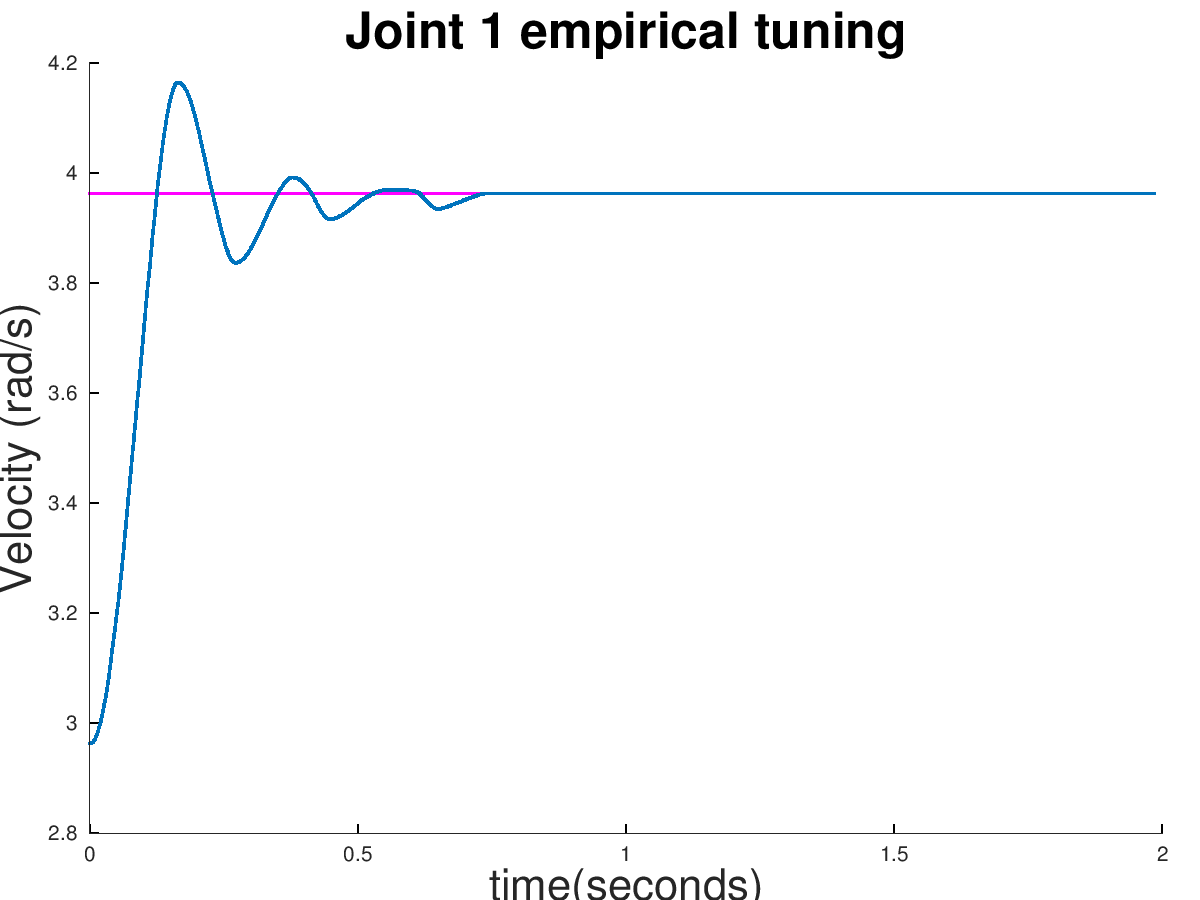
\includegraphics[width=60mm]{pictures/joint1_tuning_1.png}}
\subfigure[Slow rise time]{\label{fig:withoutoscillations}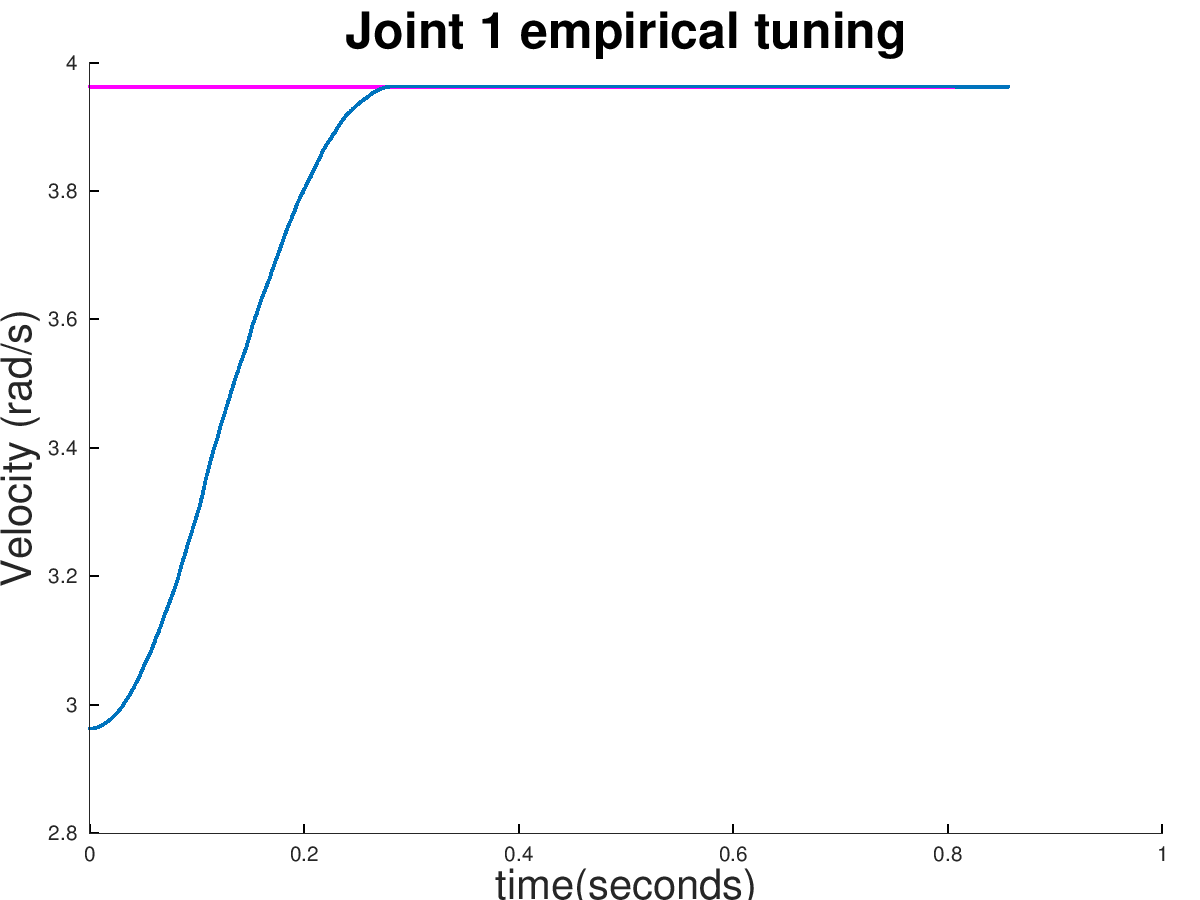
\includegraphics[width=60mm]{pictures/joint1_tuning_2.png}}
\caption{The requirements of the controller and this figure represents the tradeoff between the slow and faster rise time.}
\end{figure}

So, the trade-off has been made which avoids the oscillations and the 

\subsubsection*{Safety controller}
An upper layer has been created around the controller to prevent the damages to the manipulator joints i.e. the torque is applied when the joint is already present in it's minimum or maximum positions. This controller enables the user to apply the control algorithms to the robot safely without thinking about the mishaps that can occur in the manipulation tasks. Basically, there are three kinds of checks are being performed such as position, velocity and torque. At first, the position control check is being performed to make sure that the torque is not commanded when the joint is in it's limits. Secondly, the velocity control checks the joint velocity for avoiding the high-speed motions on the manipulator that might hit the joint limits. So, this mode stops the controller when the velocity of the joint goes over the defined threshold. Finally, the torque control check is performed in order to keep the torque input in check before commanding it to the real robot. The safety controller allows the user to set the joint torque after all these three conditions are satisfied. If any of these three conditions fail, the velocity of the manipulator joints will be set to zero where the movement of the manipulator joints will be completely stopped irrespective of the manipulation task that is getting executed by the controller then the controller stops as well due to the safety concerns. This particular safety controller interface can be used where the joint limits are applicable.

\newpage
\subsection{Trajectory generation}

Since the controller is attached in the joint-level, it is important to validate the controller with the use of a target trajectory. In this work, the trajectory way points are generated by using a simple sine wave-form where the amplitudes of the wave depends on the maximum and minimum limits of the individual joints.

\begin{equation}
q_{desired}(t) = A\cdot sin(\omega \cdot t) + \delta
\label{eq:analyticalsinewave}
\end{equation}

where $q_{desired}$ represents the analytical time based function which has all the waypoints to achieve the particular target. $2*\pi / T_f$ is the frequency $\omega_f$ of the wave, A represents the amplitude, $T_f$ is the time taken for a complete single wave and finally $\delta$ represents the offset, t represents the time taken by the controller to complete one cycle. The waypoints are fed to the controller and the measured joint values are compared against the wave to check the controller's performance. Based on the generated wave, the controller's parameters can be verified for optimality. If the joint is not following the wave close-enough, the controller gains have to be reconsidered since there are not optimum. The maximum and minimum velocity of the joints can be identified by taking the differentiation of the equation~\eqref{eq:analyticalsinewave}

\begin{equation}
\dot{q}(t) = A\cdot \omega \cdot cos(\omega \cdot t)
\label{eq:coswave}
\end{equation}

The analytical sine waveform is generated for the joint positions ($q_{desired}$) where the amplitude of the wave depends on the joint limits of the youBot manipulator. The sine wave is generated in every 10 seconds ($T_f$) and the way-points of the wave is commanded as the set-point to the cascade PI controller. The derivative operation on the function q(t) provides the velocity set-point $\dot{q}(t)$ for all the individual points in the generated sine wave.

\begin{figure}[h]
\centering
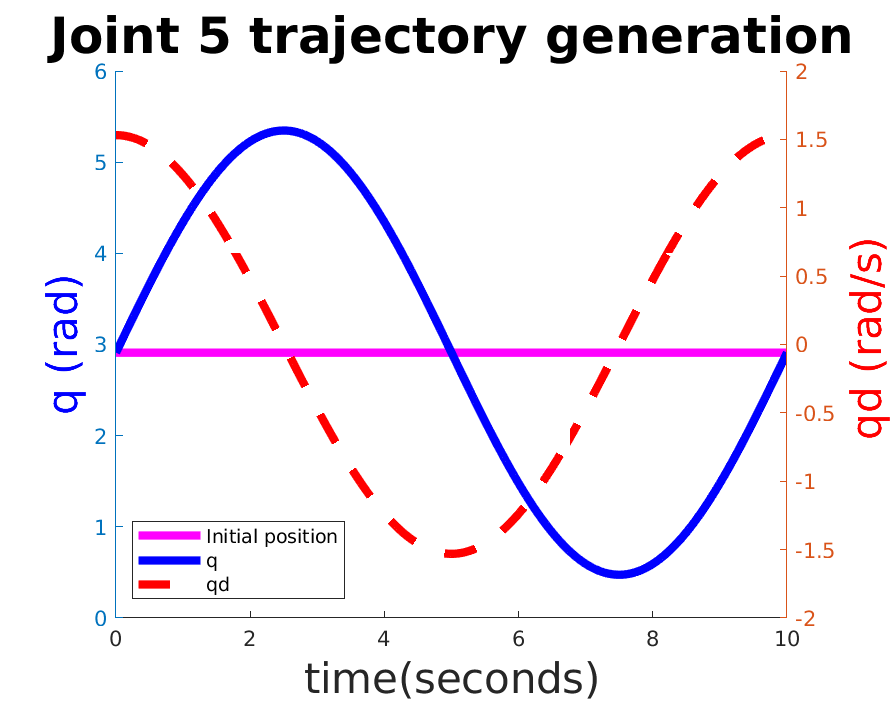
\includegraphics[width=80mm, trim=0 0 0 0]{pictures/sinewave}
\caption{The sine waveform based trajectory generation and the relative velocity qd ($\dot{q}$) is obtained by taking the derivative of q.}
\end{figure}

In order to find the maximum velocity A of the joint can be computed with the following equation. The $\omega$ is already specified where the maximum possible value for a cosine wave is 1.

\begin{equation}
\dot{q}_{max} = A\cdot \omega
\label{eq:maxjointvelocity}
\end{equation}

similarly the minimum velocity of the joint can be identified with the following formulation where the amplitude can be computed by taking the difference between the minimum joint limit with the initial position of the joint.

\begin{equation}
\dot{q}_{min} = A\cdot \omega
\label{eq:minjointvelocity}
\end{equation}

The mechanical system's introducing the delayed start comparing the waveform generation. So, the derivative of q(t) is considered as the desired velocity and it is added with the position PI's control variable (which is also a velocity). The result of this addition is commanded as the velocity set-point for the velocity PI controller. This technique helps reducing the delayed start in the mechanical systems where the desired velocity at a particular set-point is caught-up. This method can be called as computed-torque like control~\cite{Chung2016} for the purpose of accurate trajectory tracking. The above generated wave corresponds to the joint positions and the derived velocities can be used to validate the model-based controller for all the manipulator joints.
\emptypage
%%%%%%%%%%%%%%%%%%%%%%%%%%%%%%%%%%%%%%%%%%%%%%%%%%%%%%%%%%%%%%%%%%%%%%%%%%%%%%%%%%%%%%%%%%%%%
%											IMPLEMENTATION AND MEASUREMENTS																				%
%%%%%%%%%%%%%%%%%%%%%%%%%%%%%%%%%%%%%%%%%%%%%%%%%%%%%%%%%%%%%%%%%%%%%%%%%%%%%%%%%%%%%%%%%%%%%
\chapter{EXPERIMENTAL RESULTS}
\label{sec:experiments}
This chapter analyses the performances of the advanced model-based computed-torque controller. The experiments are conducted in the system that has the following configuration

\begin{flushleft}
Operating system - Ubuntu 14.04 LTS 64-bit \\
Processor - I5-7$^{th}$ generation
\end{flushleft}

\section{Model-based controller}

Torque controller is tested in youBot base at first to verify the logic of the controller before it is tested in the manipulator where the joint constraints are applicable. At first, the experiments are conducted for the safety controller interface to make sure that the safety layer is functioning properly or not in case of a logical error in the controller. The initial configuration of manipulator is assumed to be in candle as same as the 3-D model provided by the manufacturer, then the torque is commanded to the joint where the artificial position, velocity, torque limits are applied which is then replaced with the actual joint limits with a threshold of 0.5 rad in both the maximum and minimum limits of the manipulator joints. The threshold is introduced to avoid hitting the limits of the joints if the set-point is located near the joint limits. The artificial joint limits for the position, velocity, torque are 1.0 rad, 0.5 rad/s, 1.0 N.m. respectively. Once the joint limits are reached, the safety layer gets active and stops the controller to avoid any damages to the manipulator since the prolonged motion even after the breach in the safety limits could damage the system. The same experiments are conducted with the actual joint limits and the safety controller interface is breaking in the right place where the safety limits are breached. The real concern of the safety controller in high-speed motions is that the joint crosses the safety limit before the safety check is performed. The cause of this problem is that the controller is functioning in a non real-time system. 

\begin{table}[H]
\centering
\begin{tabular}{|c|c|l|l|}
\hline
\multirow{2}{*}{\textbf{PI Controller}} & \multicolumn{1}{l|}{\multirow{2}{*}{\textbf{Gains}}} & \multicolumn{2}{l|}{\textbf{Joint No.}}                           \\ \cline{3-4} 
                                        & \multicolumn{1}{l|}{}                                & \multicolumn{1}{c|}{\textbf{4}} & \multicolumn{1}{c|}{\textbf{5}} \\ \hline
\multirow{2}{*}{\textbf{Position}}      & P                                                    & 0.820                           & 1.900                           \\ \cline{2-4} 
                                        & I                                                    & 0.063                           & 0.033                           \\ \hline
\multirow{2}{*}{\textbf{Velocity}}      & P                                                    & 2.900                           & 1.500                           \\ \cline{2-4} 
                                        & I                                                    & 0.180                           & 0.120                           \\ \hline
\end{tabular}
\caption{Controller gains for the joints 4,5 after the empirical tuning procedure}
\end{table}

Basic approach is experimented prior to the alternate approach. The model-based controller based on the basic approach is successfully achieving the gravity compensation in the youBot manipulator that is based on KDL ID solver and the cascaded PI controller is also tested in the youBot manipulator. The main observation from this experiment is that the control variable $\ddot{q}$ computed by the cascaded controller is fed as an acceleration input to the KDL based solver where the model torques are generated which results in a very minimal torque ($10^{-5} N.m.$). These model torques were not sufficient enough to move the joints of the manipulator to the desired configuration. The reason behind this problem is that the inertial parameters are not accurate and rotor inertia should also be considered rather than just considering the links' moments of inertia. The static friction compensation is also experimented to move the joint from the equilibrium state and the identified static friction values from the previous work~\cite{RnD2Rajagopal} were not sufficient to move the joint from the rest state. So, the static friction value for the joints are increased to overcome the static friction on the manipulator joints. Once the joint started moving, the Coulomb friction torques were added with the model torques that compensates the dynamic friction. The alternate method that is used in this work is not having the friction compensation with it due to the fact that the model does only two things such as the gravity compensation and accounting the bias forces. Since the cascaded controller is implemented in this work, it is important to tune both the position and velocity controller gains to the optimum, empirically. The inner-loop and outer-loop controller has been tested with the different velocity set-points to check whether the tuned parameters are optimum or not. The empirical tuning of the controller gains for both the inner-loop and outer-loop with the velocity of 0.5 rad/s are depicted in the Figures~\ref{fig:innerloop_tuning0pt5rads}~\ref{fig:outerloop_tuning0pt5rads} respectively for the joint number 5. Since the measured velocity from the encoders are quite noisy as it is shown in Fig.~\ref{fig:innerloop_tuning0pt5rads}, the measured data is smoothed with the moving average filter that filters the noise with the window size 10. The smoothed data is helpful in understanding whether the set-point in the inner-loop has reached or not. The steady-state error with the threshold of 0.02 rad/s are assumed to be accepted in the inner-loop when tuning the controller gains due to the presence of noise but the ultimate goal of this project is to achieve the zero steady-state error. The outer-loop tuning is quite straight-forward where the joint  position set-point 0.5 rad is commanded to the joint and the result of the movement confirms the optimality of the controller gains. The additional tuning experiments with the different position and velocity set-points for the joint 5 can be found in the appendix~\ref{sec:appendixD}. 

\begin{figure}[H]
\centering     %%% not \center
\subfigure[Inner loop tuning]{\label{fig:innerloop_tuning0pt5rads}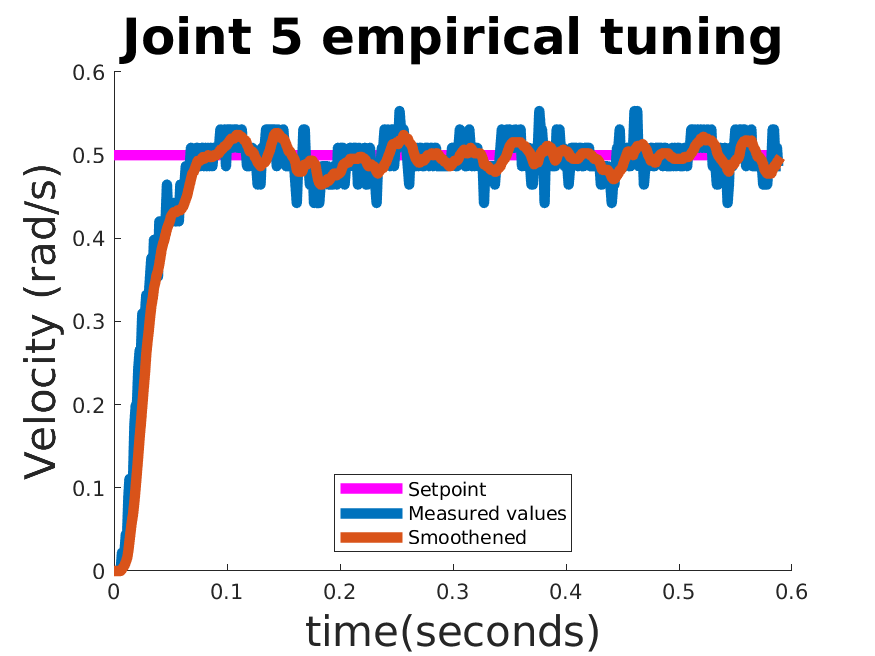
\includegraphics[width=70mm]{pictures/joint5_innerloop_0pt5rads}}
\subfigure[Outerloop tuning]{\label{fig:outerloop_tuning0pt5rads}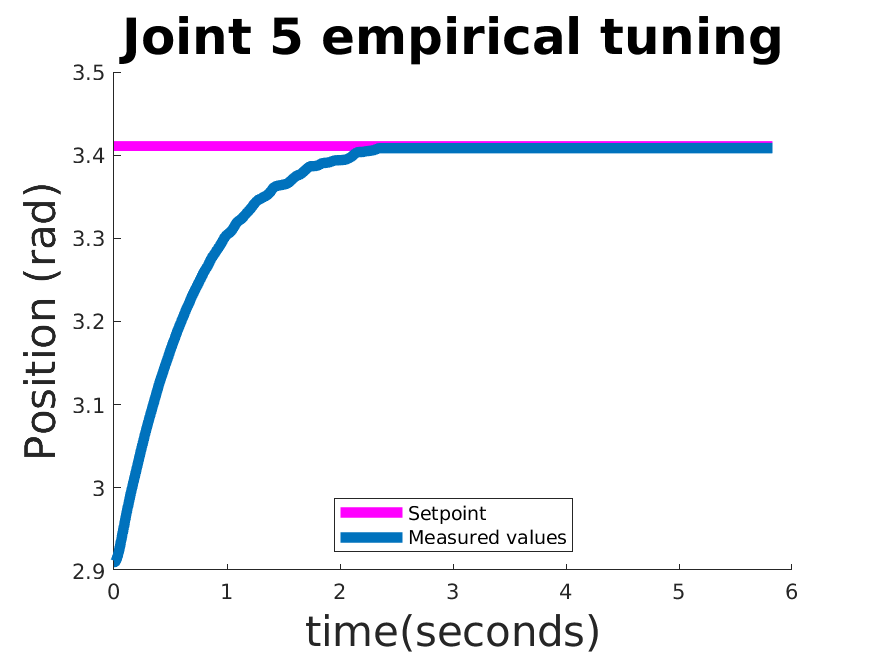
\includegraphics[width=70mm]{pictures/joint5_outerloop_0pt5rad}}
\caption{Inner, outer loop tuning for joint 5 with the velocity, position set-points of 0.5 rad/s, 0.5 rad respectively}
\end{figure}

After the controller gains are tuned to optimal values based on the set-points and the controller response, the individual joints of the manipulator can be evaluated with the analytical sine wave form as depicted in Fig.~\ref{fig:trajectorytrackingjoint5} since the computed-torque controller is attached in the joint level. The way-points of the sine waveform are generated in accordance with the controller frequency. In each and every cycle of the controller, a new position set-point (the way-points of the sine waveform) is commanded and the response is observed for the purpose of evaluation. 

\begin{figure}[H]
\centering
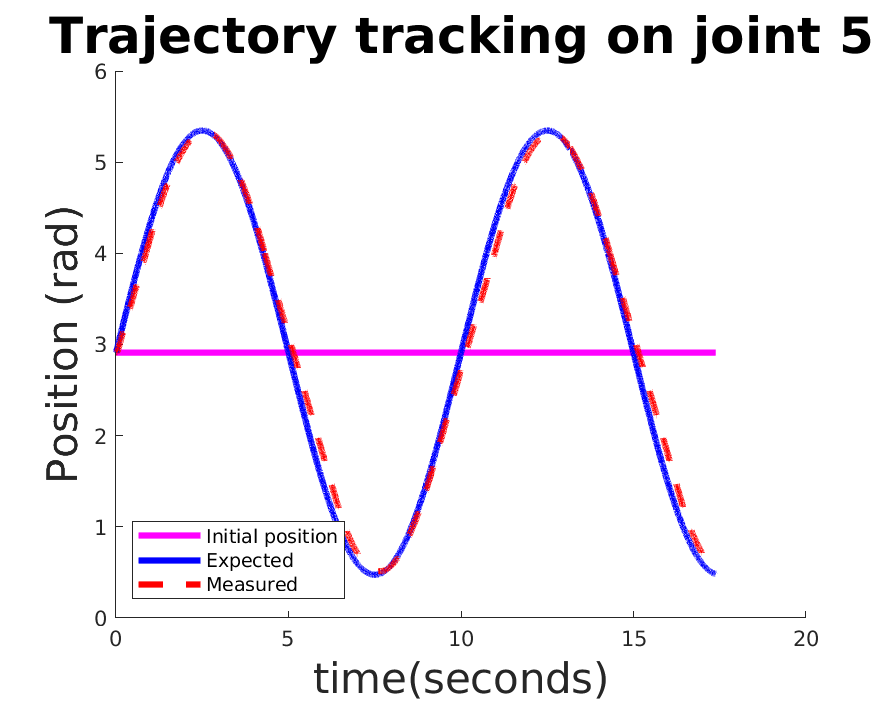
\includegraphics[width=90mm, trim=0 20 0 20]{pictures/joint5_trajectory}
\caption{Trajectory tracking experiment using the sine wave on joint 5}
\label{fig:trajectorytrackingjoint5}
\end{figure}

The error between the set-point and the controller response for all the way-points of the sine wave are depicted in Fig.~\ref{fig:trajectorytrackingerrorjoint5}. The maximum error that has been observed in joint number 5 is 0.3171 rad at some point in time. 

\begin{figure}[H]
\centering
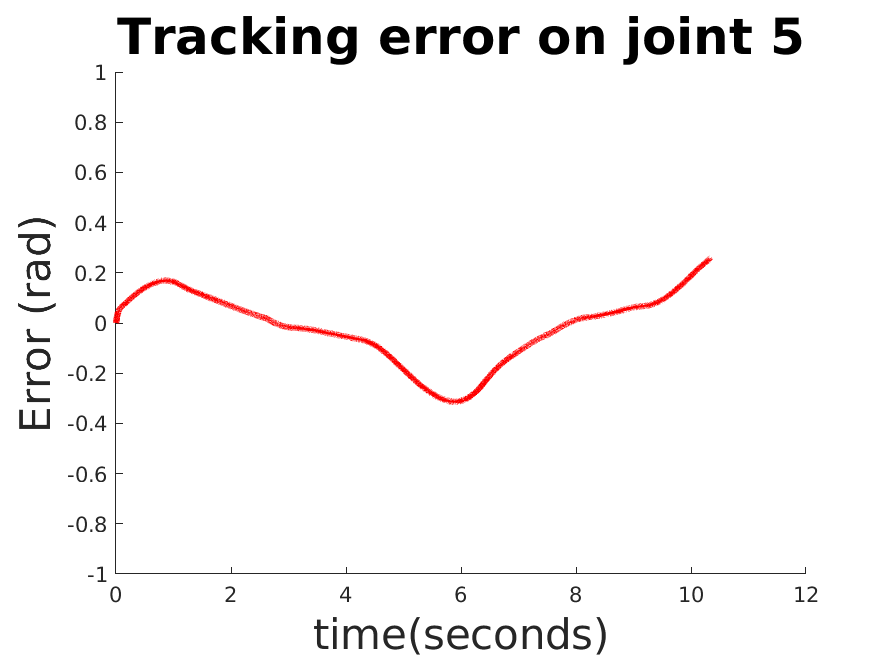
\includegraphics[width=90mm, trim=0 20 0 20]{pictures/joint5_trajectoryerror}
\caption{Trajectory tracking error on joint 5}
\label{fig:trajectorytrackingerrorjoint5}
\end{figure}

The controller gains are tuned for the joint 4 as depicted in the Figures~\ref{fig:innerloop_tuning0pt5rads_joint4}~\ref{fig:outerloop_tuning0pt5rads_joint4} which follows the same procedure that has been followed for the joint number 5. 

\begin{figure}[H]
\centering     %%% not \center
\subfigure[Inner loop tuning]{\label{fig:innerloop_tuning0pt5rads_joint4}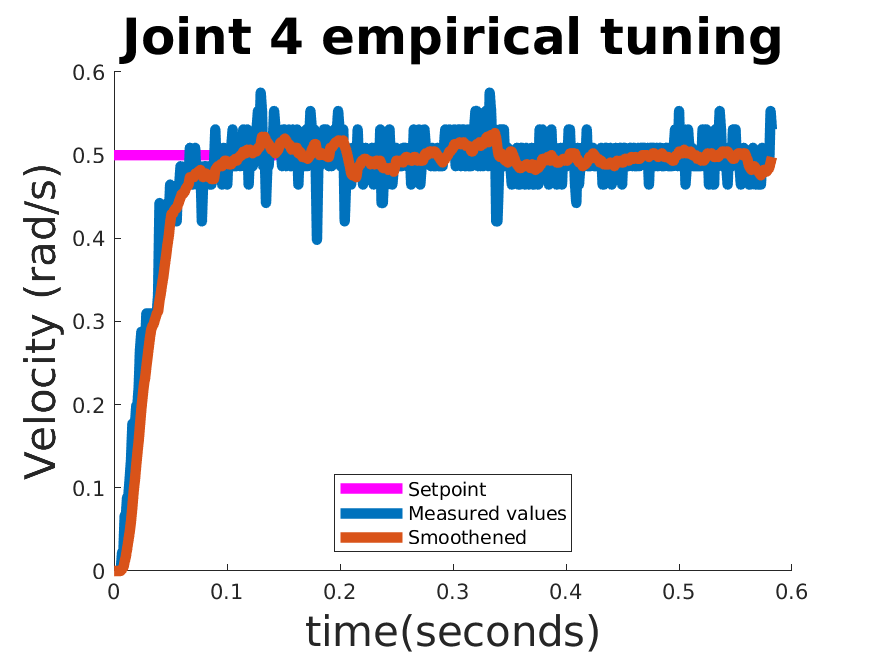
\includegraphics[width=70mm]{pictures/joint4_innerloop_0pt5rads}}
\subfigure[Outerloop tuning]{\label{fig:outerloop_tuning0pt5rads_joint4}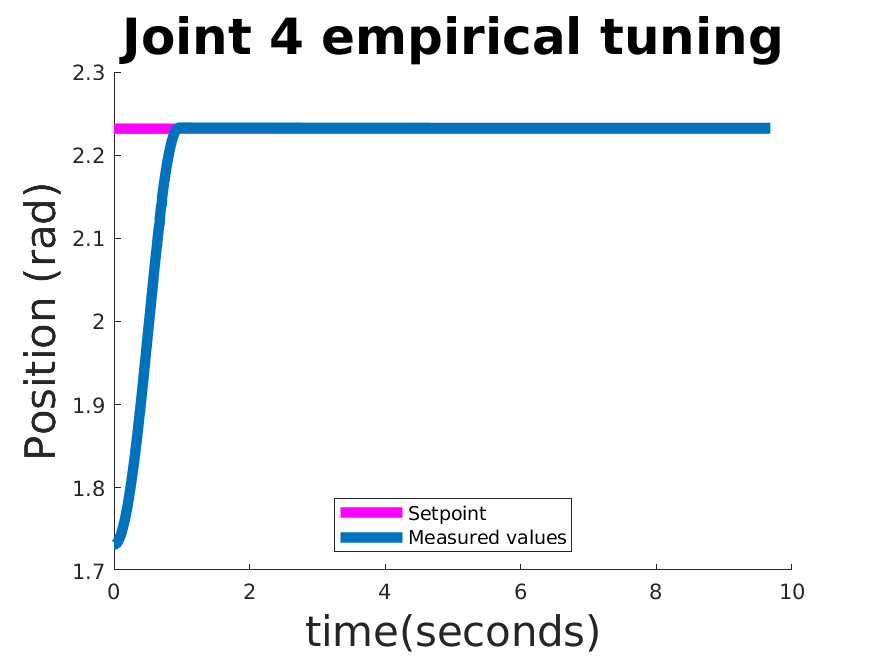
\includegraphics[width=70mm]{pictures/joint4_outerloop_0pt5rad}}
\caption{Inner, outer loop tuning for joint 4 with the velocity, position set-points of 0.5 rad/s, 0.5 rad respectively}
\end{figure}

\begin{figure}[H]
\centering
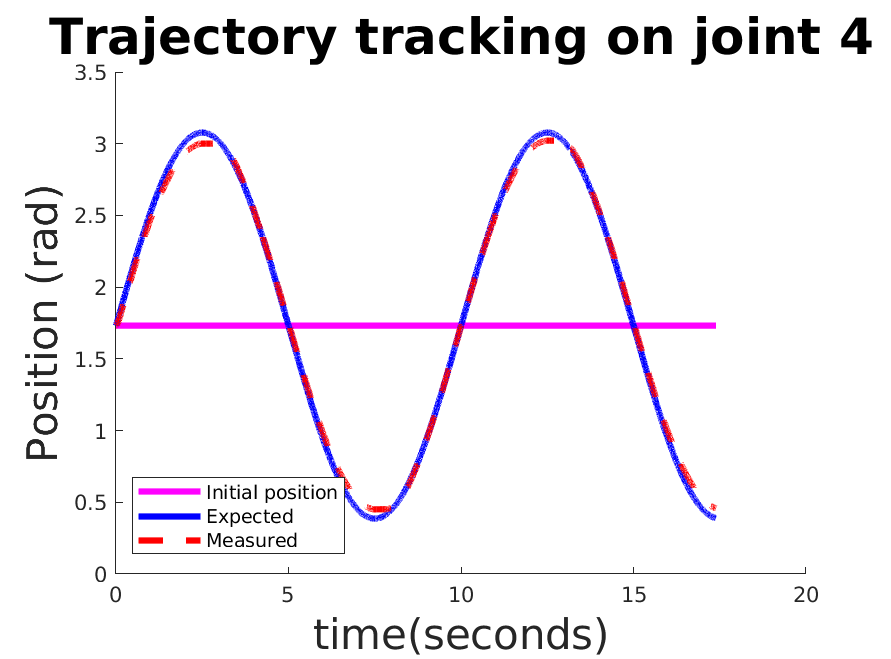
\includegraphics[width=90mm, trim=0 20 0 20]{pictures/joint4_trajectory}
\caption{Trajectory tracking experiment using the sine wave on joint 4}
\label{fig:trajectorytrackingjoint4}
\end{figure}

The error between the set-point and the controller response for all the way-points of the sine wave are depicted in Fig.~\ref{fig:trajectorytrackingerrorjoint4}. The maximum error that has been observed in joint number 4 is 0.0779 rad at some point in time. 

\begin{figure}[H]
\centering
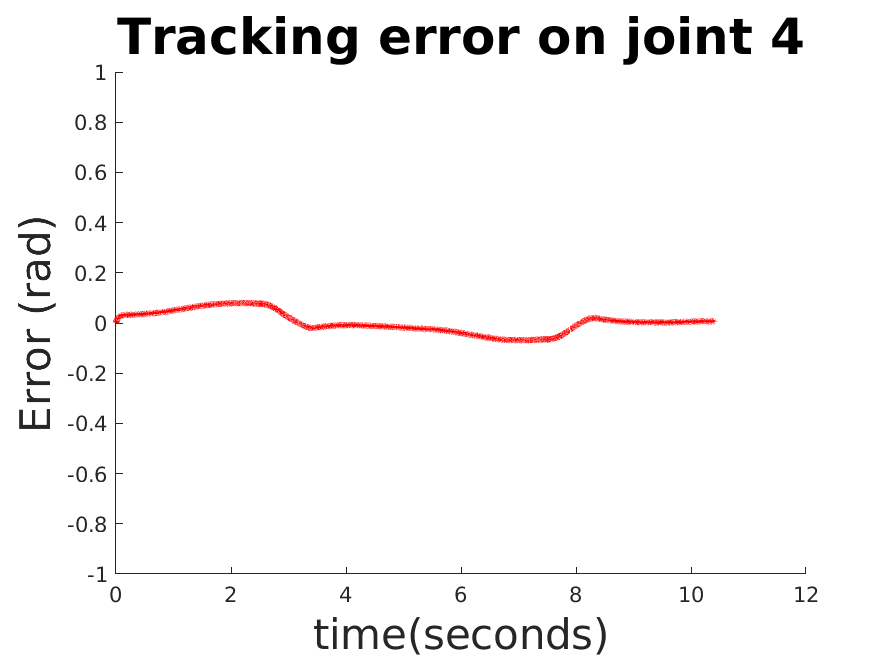
\includegraphics[width=90mm, trim=0 20 0 20]{pictures/joint4_trajectoryerror}
\caption{Trajectory tracking error on joint 4}
\label{fig:trajectorytrackingerrorjoint4}
\end{figure}

The trajectory tracking error is caused due to many reasons such as the controller gains are not be optimal yet hence the tuning has to be re-considered, the presence of the cascaded controller where the optimality of the inner-loop control gains are suffering due to the noise in the measured data. The following Fig.~\ref{fig:ratiojoint4} depicts the model, controller torques w.r.t. the position of joint 4.

\begin{figure}[H]
\centering
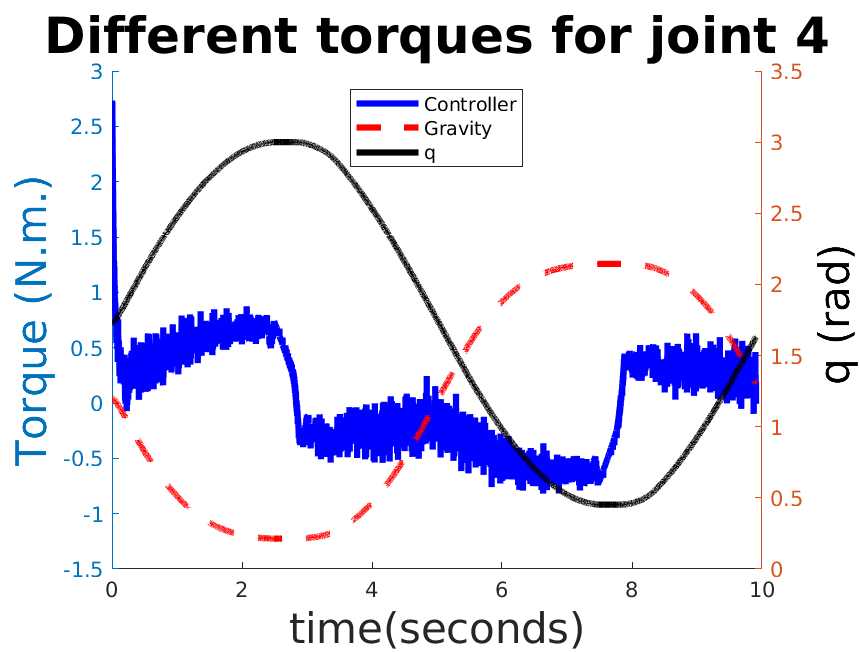
\includegraphics[width=90mm, trim=0 0 0 0]{pictures/joint4_ratio}
\caption{Modeled torque and controller torques are shown w.r.t. time along with the angular position for joint 4}
\label{fig:ratiojoint4}
\end{figure}

It can be clearly seen that torque generated by the model do not have high frequency noise as expected. Again, the controller handles the disturbances in the manipulator joints producing high-frequency components. An important cause of this problem is that the model discrepancies introduce deviations in torque prediction which in-turn has a huge impact on the advanced model based controller. The friction compensation terms in the dynamic model would improve the controller's performance further. Though the dynamic model is incomplete, the controller is able to follow the trajectories close-enough with a minimal deviations. The non real-time system is used for the development that produces latency issues in the feedback-control system. 

\section{Inertial parameter estimation}

The inertial model parameters provided by the manufacturers are inaccurate and the identification of the model parameters are not complete. It is decided to go with the mass and CoM where the rotational inertia parameters are ignored in the system model of the youBot manipulator. The link parameters without the rotational inertia has been tested on the real robot for the gravity compensation and the joints are not sliding due to gravitational pull hence the link properties of the dynamic model in Orocos KDL excludes the rotational inertia in the computations.
\emptypage
%%%%%%%%%%%%%%%%%%%%%%%%%%%%%%%%%%%%%%%%%%%%%%%%%%%%%%%%%%%%%%%%%%%%%%%%%%%%%%%%%%%%%%%%%%%%%
%																		CONCLUSION 																							%
%%%%%%%%%%%%%%%%%%%%%%%%%%%%%%%%%%%%%%%%%%%%%%%%%%%%%%%%%%%%%%%%%%%%%%%%%%%%%%%%%%%%%%%%%%%%%
\chapter{CONCLUSIONS AND FUTURE WORK}
\label{sec:conclusion}

In this work, an attempt has been made to achieve the accurate trajectory tracking control on the youBot manipulator. Initially, the plan was to implement and test the controller in Simbody visualizer but the manipulator has an impact due to gravity and it starts sliding overtime where it is supposed to stay in the candle configuration. So, the conclusion on this module is that the model used in both the Simbody and KDL libraries are the same but there is a mismatch between these two libraries in the semantic level introduces such a problem. It is then decided to implement the controller in the youBot base at first to verify the correctness of both the safety and the cascade control. The model-based controller requires two important modules such as the model of the system and mainly the controller. It is not just enough to have the model of the system rather it has to be accurate enough to predict the feed-forward torques of the real system precisely. For which, the identification procedure is considered and the findings of the same are presented. It is really important to understand the semantics of the rigid-body algorithms given by different authors before implementing the algorithm itself. The lesson learned from the identification modules' findings are that the semantics differ from one author to another and the implicit conventions must be decoded before implementing the rigid-body algorithms provided by the authors. So, the identification procedure is partially completed with the findings and the model parameters can be used effectively once the identification of the parameters are  complete. The Orocos KDL library is used for computing the model torques and this work has an important finding in the KDL frame diagram. The author mentions that the CoM point and the inertial frame can be located w.r.t. the root frame. But this representation is mismatching with the actual implementation where the inertial frame, CoM point can only be located w.r.t. the tip frame. The next important contribution of this work is the control module and there are two kinds of control schemes got investigated and implemented in this work. The alternate approach with the simple computed-torque controller is selected for proof of concept. The cascade PI control is implemented with KDL based feed-forward torque computation. It is necessary that the controller gains of the joints 4, 5 are tuned to the optimum empirically for achieving the better performance in tracking. The same procedure can be followed for all the other manipulator joints. An important contribution of this work is the inclusion of the safety control layer which is responsible for preventing any damages to the system. The safety controller shows promising results but there is a presence of the latency problem since the implementation is done in the non real-time operating systems. Although the basic approach does the gravity compensation, the inaccurate rotational inertial parameters causes the problem in the torque prediction. It is also observed that the rotor moments of inertia has to be accounted in the model based controllers since the current system accounts only for the links' moments of inertia. The friction has also been investigated and tested with the basic approach where the static friction and Coulomb frictions are modeled and compensated in the manipulator joints based on the assumptions made. In spite of having the inaccurate model parameters of the system in this work, the controller has been evaluated in the joint level with the use of the simple sine waveform and the results were presented. The tracking errors on joint 4, 5 are 0.3171 N.m. and 0.0779 N.m. respectively. 

\section*{Future work}

The trajectory tracking control can be improved by adapting the current implementation with the following changes in the model-based controller.

\begin{itemize}
\item The real-time operating system can be used for avoiding the latency issues in the controller.
\item The model discrepancies need to be resolved for which the identification procedure with the optimal excitation trajectories must be achieved, then the inaccurate model parameters can be replaced with the identified dynamic model parameters. The semantics involved in the rigid-body algorithm has to be corrected in both the motion and force transforms based on the findings of this work.
\item Moving back to the actual computed-control scheme that is presented in the \textbf{basic approach} since this is the actual computed-torque control method. 
\item One of the important aspects of the unmodeled dynamics is called friction. So, the friction observer can be added to the control scheme as given in the basic approach.
\end{itemize} 

\emptypage

% bibliography and appendixes
%%%%%%%%%%%%%%%%%%%%%%%%%%%%%%%%%%%%%%%%%%%%%%%%%%%%%%%%%%%%%%%%%%% 
%                                                                 %
%                           BIBLIOGRAPHY                          %
%                                                                 %
%%%%%%%%%%%%%%%%%%%%%%%%%%%%%%%%%%%%%%%%%%%%%%%%%%%%%%%%%%%%%%%%%%% 
 
%This method produces a numbered bibliography where the numbers
%correspond to the \cite commands in the text. See the LaTeX manual.
\specialhead{\bibname}

\bibliographystyle{abbrv} % mit Buchstaben
%\bibliographystyle{plain} % normal
%\bibliographystyle{unsrt} % in reinfolge des Textes
%\bibliographystyle{abbrv} % wie plan , nur abgek�rtz

\begin{singlespace}

\nocite{4586493}
\nocite{34773}
\nocite{muggler2013torque}
\nocite{RnD2Rajagopal}
\nocite{craig2005introduction}
\nocite{geometicsemanticspart1}
\nocite{geometicsemanticspart2}
\nocite{smits2011kdl}
\nocite{kukamanipulator}
\nocite{temelp}
\nocite{sherman2011simbody}
\nocite{torquecontrol}
\nocite{Chung2016}
\nocite{Atkeson}
\nocite{swevers}
\nocite{cascadedcontrol}
\nocite{featherstone2014rigid}
\nocite{corberan2012haptic}
\nocite{youbotdriver_architecture}
\nocite{youbotdriver}
\nocite{SweversJ1997Orea}
\nocite{vantilt2015optimal}
\nocite{trajectorytracking_nn}
\nocite{sellers2001overview}
\nocite{astrom1995pid}
\nocite{boyd2004convex}
\nocite{traversaro2016multibody}
\nocite{olsson1998friction}
\nocite{de2012theory}
\nocite{friction}

\bibliography{bibtex}

\end{singlespace}
   

\emptypage
%%%%%%%%%%%%%%%%%%%%%%%%%%%%%%%%%%%%%%%%%%%%%%%%%%%%%%%%%%%%%%%%%%%
%                                                                 %
%                            APPENDICES                           %
%                                                                 %
%%%%%%%%%%%%%%%%%%%%%%%%%%%%%%%%%%%%%%%%%%%%%%%%%%%%%%%%%%%%%%%%%%%
 
\appendix    % This command is used only once!
%\addcontentsline{toc}{chapter}{APPENDICES}             %toc entry  or:
\addtocontents{toc}{\parindent0pt\vskip12pt APPENDICES} %toc entry, no page #
\let\cleardoublepage\clearpage
\chapter{YouBot driver}
\label{sec:appendixA}
The youBot base or the manipulator can be controlled in three different modes as discussed in the introduction section. The interface details~\cite{youbotdriver}~\cite{youbotdriver_architecture} of the driver that are used in this project are briefed in this section. It is important to obtain the handle reference for the youBot manipulator or the base in order to command the data or retrieve the sensed data from the joints. The handle to the youBot manipulator can be obtained by creating an object to the following class

\begin{verbatim}
youbot::YouBotManipulator *youbotArm(Arm_name, Path_to_config_directory);
\end{verbatim}

and the handle for the youBot base can be obtained similarly

\begin{verbatim}
youbot::YouBotBase *youbotBase(Base_name, Path_to_config_directory);
\end{verbatim}

This work explains only the implementation details of the youBot manipulator and the youBot base can also be controlled in the similar way. The robot joints can be controlled individually or collectively. The position/velocity/torque commands to the joints has to be prepared and can be given as follows

\begin{verbatim}
vector<youbot::JointAngleSetpoint> jointAngleCommands(Total_Joints);
vector<youbot::JointVelocitySetpoint> jointVelocityCommands(Total_Joints);
vector<youbot::JointTorqueSetpoint> jointTorqueCommands(Total_Joints);
\end{verbatim}

where Total\_Joints represents the number of joints in the manipulator. The measured joint information for all the joints can be read with the use of the following classes

\begin{verbatim}
vector<youbot::JointSensedAngle> jointAnglesMeasured(Total_Joints);
vector<youbot::JointSensedVelocity> jointVelocitiesMeasured(Total_Joints);
vector<youbot::JointSensedTorque> jointTorquesMeasured(Total_Joints);
\end{verbatim}

With the use of the above classes, it is now possible to set or get the angle (in radians) for all the joints of manipulator with the use of the following methods

\begin{verbatim}
youBotArm->setJointData(jointAngleCommands);
youBotArm->getJointData(jointAnglesMeasured);
\end{verbatim}

The velocity, torque modes can also be controlled similarly with the use of the above given methods. 

\chapter{Orocos KDL}
\label{sec:appendixB}

At first the kinematic chain of the youBot manipulator has to be created as follows

\begin{verbatim}
KDL::Chain kinematicChain;
\end{verbatim}

The manipulator is represented by the kinematic chain of rigid bodies or segments. The next step is to add the segments of the manipulator to the kinematic chain that has been created in the previous step. 

The segments can be created by instantiating an object to the following class

\begin{verbatim}
KDL::Segment segment(name, joint_axis, frame, rigid_body_inertia);
\end{verbatim}

where the segment defines both the joint information and link properties which are then added to the chain by using the following method

\begin{verbatim}
kinematicChain.addSegment(segment);
\end{verbatim} 

Once the complete kinematic chain of the manipulator is created, the kinematics and dynamics of kinematic chains can be computed. The Orocos KDL library provide solvers for both the forward and inverse kinematics computations. This work made use of the forward kinematics solver to find the end-effector's pose and the solver can be instantiated and invoked as given below.

\begin{verbatim}
KDL::ChainFkSolverPos_recursive::JntToCart(q, T)
\end{verbatim} 

where q represents the joint position inputs for the manipulator joints and T represents the frame (KDL::Frame) that gives the pose information of the end-effector. The dynamics of the kinematic chain can be computed by using the recursive Newton-Euler formulation which is implemented based on the article~\cite{featherstone2014rigid}. Though the semantics used is same as the article, there is an important difference in the semantics of the algorithm in KDL comparing the article, i.e. In ~\cite{featherstone2014rigid}, author uses the spatial vector transforms in the algorithm whereas KDL does not uses the spatial form. The ID solver which is used in KDL can be invoked as follows

\begin{verbatim}
KDL::ChainIdSolver_RNE idsolver;
idsolver.CartToJnt(position, velocity, acceleration, wrench, torques);
\end{verbatim}

\chapter{Simbody}
\label{sec:appendixC}

At first the visualizer has to be created with the use of the class SimTK::Visualizer where the properties can be adjusted based on the system needs and an event reporter (PeriodicEventReporter) is attached to handle the events of the system at the defined intervals. The time stepper (SimTK::TimeStepper) uses SimTK::RungeKuttaMersonIntegrator to take the system forward through time. The system is initialized after the system model is created. The forces can be commanded to the manipulator joints as generalized forces by using the class SimTK::GeneralForceSubSystem. The more detailed reference can be found in\footnote{\url{https://simtk.org/api_docs/simbody/3.5/namespaceSimTK.html}} and the implementation details are specified as follows. In Simbody, the multi-body system is created at first and the sub-systems are attached for the further operations. The system has a subclass SimTK::MultibodySystem to work with the general multi-body systems along with the sub-system SimTK::SimbodyMatterSubSystem which is responsible for defining all the rigid bodies in the system. 

\begin{verbatim}
SimTK::MultibodySystem system;
SimTK::SimbodyMatterSubSystem matterSubSystem(system);
\end{verbatim}

The gravity can be simulated with the use of the following class

\begin{verbatim}
SimTK::Force::Gravity gravity = SimTK::Force::Gravity();
\end{verbatim}

A rigid body can be created and the link properties can be attached with the help of the following classes

\begin{verbatim}
SimTK::Body rigid_body;
rigid_body = SimTK::Body::Rigid(SimTK::MassProperties(mass, CoM, Inertia));
\end{verbatim}

The joints can be created with the use of the MobilizedBody class

\begin{verbatim}
SimTK::MobilizedBody body(Number_of_joints);
\end{verbatim}

Before attaching the rigid bodies to the sub-system, it is important to attach the base body to the ground (parent body) which is the origin by using the weld joint

\begin{verbatim}
body = SimTK::MobilizedBody::Weld();
\end{verbatim}

The revolute joints can be attached to the mobilized body with the help of the Pin  class which attaches a new body to the system with the one DoF constraint to the predecessor.

\begin{verbatim}
body = SimTK::MobilizedBody::Pin();
\end{verbatim}

The joint information such as position, velocity and acceleration are retrieved from the state of the system that gets updated in a periodic manner. The torque sensor has been created in this work with the use of the SimTK interface that measures the gravitational, bias and the custom forces from the multi body system. It is possible to command the generalized coordinate with the particular motion as a function which can be step or sinusoid use of the following class

\begin{verbatim}
SimTK::Constraint::PrescribedMotion
\end{verbatim}

The two-link manipulator has been created to test the prescribed motion in this work to verify the semantic correctness and setting the joint positions required the update in the state variable which is a constant in Simbody and the setup for the 2-link manipulator is depicted in Fig.~\ref{fig:simbody_2link}.

\begin{figure}[H]
\centering
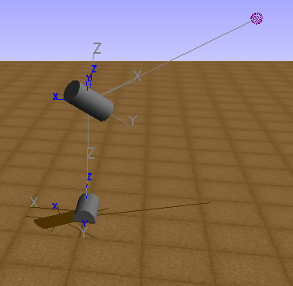
\includegraphics[width=50mm, trim=0 0 0 0]{pictures/simbody_2link_manipulator}
\caption{Two-link manipulator is constructed with the cylinder objects in Simbody visualizer for commanding the prescribed motion to the mobilizer}
\label{fig:simbody_2link}
\end{figure}

\chapter{Tuning of the controller gains}
\label{sec:appendixD}

\begin{figure}[H]
\centering     %%% not \center
\subfigure[Inner loop tuning]{\label{fig:joint5_innerloop_1rads}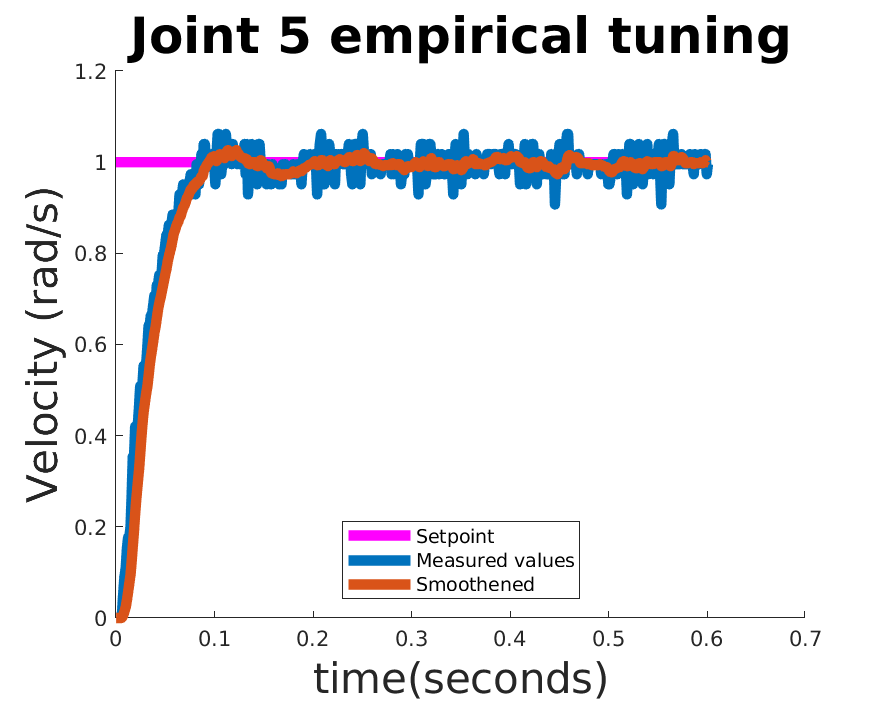
\includegraphics[width=70mm]{pictures/joint5_innerloop_1rads}}
\subfigure[Outerloop tuning]{\label{fig:joint5_outerloop_1rad}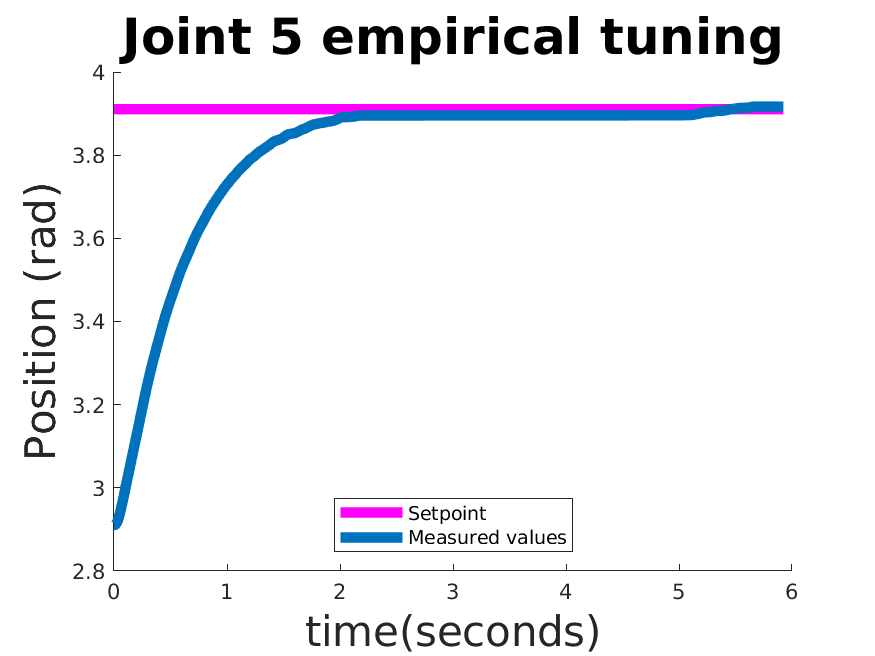
\includegraphics[width=70mm]{pictures/joint5_outerloop_1rad}}
\caption{Inner, outer loop tuning for joint 5 with the velocity, position set-points of 1.0 rad/s, 1.0 rad respectively}
\end{figure}

\begin{figure}[H]
\centering     %%% not \center
\subfigure[Inner loop tuning]{\label{fig:joint5_innerloop_1pt5rads}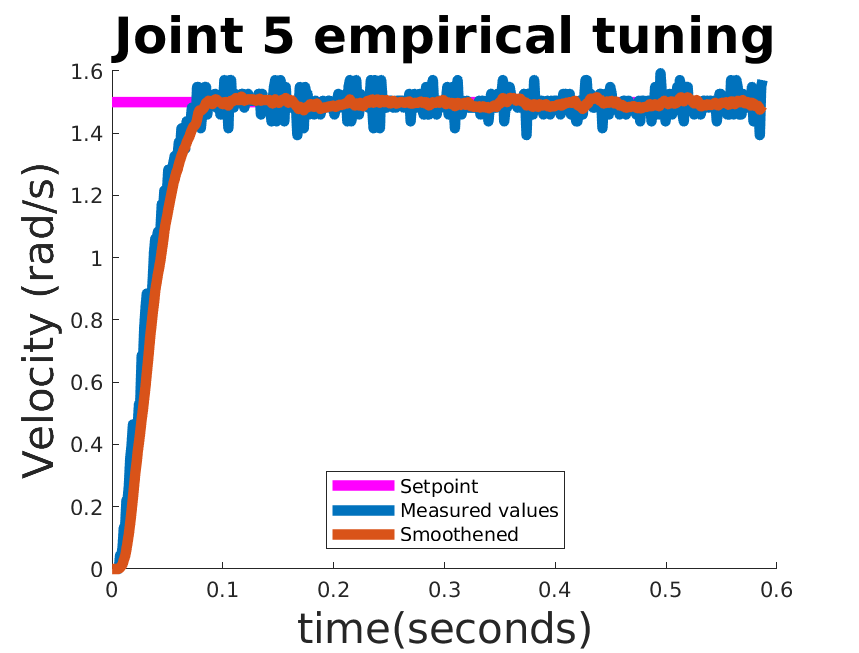
\includegraphics[width=70mm]{pictures/joint5_innerloop_1pt5rads}}
\subfigure[Outerloop tuning]{\label{fig:joint5_outerloop_1pt5rad}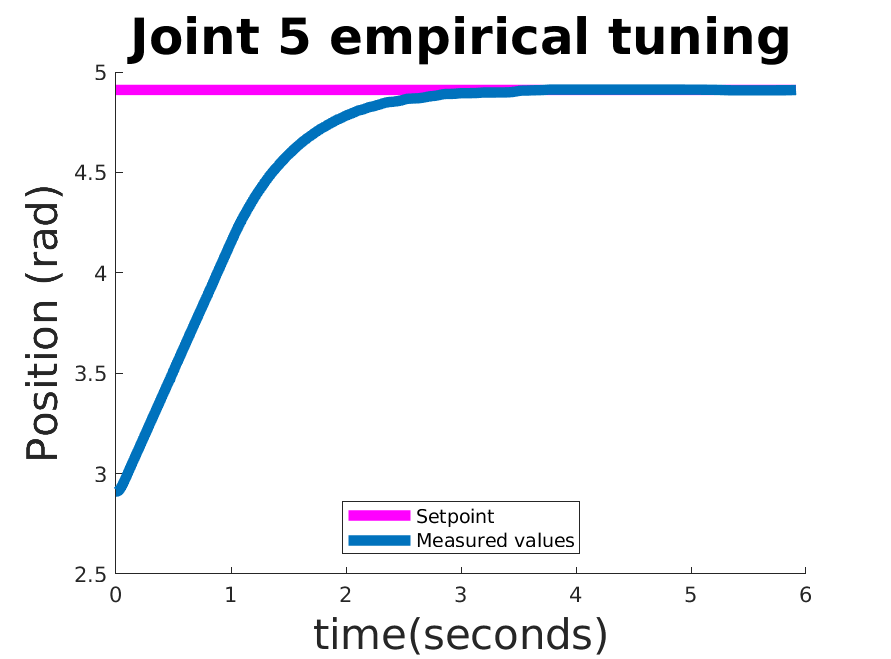
\includegraphics[width=70mm]{pictures/joint5_outerloop_2rad}}
\caption{Inner, outer loop tuning for joint 5 with the velocity, position set-points of 1.5 rad/s, 1.0 rad respectively}
\end{figure}


\emptypage
\emptypage

\end{document}
